% ============================================================
%  TESIS MECA — UNIANDES
%  ¿Pueden los datos geoespaciales públicos mejorar la
%  predicción de la vulnerabilidad a la pobreza?
%  Evidencia para hogares colombianos con base en la ELCO
%
%  Objetivo: ≤ 35 páginas de texto (sin contar portada,
%  resumen ejecutivo, tablas en apéndice ni referencias)
%  Distribución aproximada por sección (ver comentarios)
% ============================================================

\documentclass[12pt, letterpaper]{article}

% ── Paquetes ──────────────────────────────────────────────
\usepackage[utf8]{inputenc}
\usepackage[T1]{fontenc}
\usepackage[spanish, es-nodecimaldot]{babel}
% El paquete babel-spanish nombra por defecto los flotantes de tipo
% "table" como "Cuadro", mientras el texto los cita como "Tabla"
% (convención más usual en este tipo de trabajo). Se unifica en "Tabla".
\addto\captionsspanish{\renewcommand{\tablename}{Tabla}}
\usepackage[
  top=2.5cm, bottom=2.5cm,
  left=3cm,  right=2.5cm
]{geometry}
\usepackage{setspace}
\usepackage{microtype}
\usepackage{lmodern}

% Matemáticas
\usepackage{amsmath, amssymb, amsthm}
\newtheorem{proposition}{Proposición}

% Figuras y tablas
\usepackage{graphicx}
\usepackage{booktabs}
\usepackage{longtable}
\usepackage{caption}
\usepackage{subcaption}
\usepackage{float}
% Alinea las paginas dedicadas exclusivamente a floats (ej. tablas [tp]
% grandes que no caben junto a texto) hacia ARRIBA en vez de centrarlas
% verticalmente (comportamiento por defecto del kernel de LaTeX,
% \@fptop/\@fpbot = \vfil) -- evita el espacio en blanco antes de tablas
% largas como las de la Seccion 5.1.
\makeatletter
\setlength{\@fptop}{0pt}
\setlength{\@fpbot}{0pt plus 1fil}
\makeatother
% Mismo objetivo: floats grandes (tablas consolidadas de la Seccion 5.1)
% quedan mas dispuestos a compartir pagina con texto en vez de reservar
% una pagina exclusiva para ellos solos.
\renewcommand{\topfraction}{0.85}
\renewcommand{\textfraction}{0.1}
\renewcommand{\floatpagefraction}{0.75}
\usepackage{rotating}
\usepackage{multirow}

% Espaciado alrededor de figuras/tablas flotantes -- reducido frente al
% default de LaTeX (~20pt) para no perder tanto espacio de página con la
% cantidad de figuras/tablas [H] de este documento.
\setlength{\textfloatsep}{10pt plus 2pt minus 2pt}
\setlength{\intextsep}{8pt plus 2pt minus 2pt}
\setlength{\floatsep}{8pt plus 2pt minus 2pt}
\setlength{\abovecaptionskip}{4pt}
\setlength{\belowcaptionskip}{2pt}

% Espaciado de encabezados de sección -- reducido frente al default de
% \emph{article} (\section ~3.5ex antes/2.3ex después, \subsection
% ~3.25ex/1.5ex) para reclamar espacio de página en un documento con
% muchas subsecciones.
\usepackage{titlesec}
\titlespacing*{\section}{0pt}{2.2ex plus 0.5ex minus 0.2ex}{1.2ex plus 0.2ex}
\titlespacing*{\subsection}{0pt}{1.8ex plus 0.5ex minus 0.2ex}{0.9ex plus 0.2ex}
\titlespacing*{\subsubsection}{0pt}{1.4ex plus 0.5ex minus 0.2ex}{0.6ex plus 0.2ex}

% Colores e hipervínculos
\usepackage[dvipsnames]{xcolor}
\usepackage[
  colorlinks = true,
  linkcolor  = NavyBlue,
  citecolor  = NavyBlue,
  urlcolor   = NavyBlue
]{hyperref}

% Bibliografía
\usepackage[
  backend    = biber,
  style      = apa,
  sorting    = nyt,
  natbib     = true
]{biblatex}
\addbibresource{referencias.bib}   % <-- tu archivo .bib

% Encabezados
\usepackage{fancyhdr}
\pagestyle{fancy}
\fancyhf{}
\rhead{\small\textit{Vulnerabilidad a la pobreza y datos geoespaciales}}
\lhead{\small\textit{Melo, J. (2026)}}
\cfoot{\thepage}
\renewcommand{\headrulewidth}{0.4pt}

% Espaciado
\onehalfspacing

% ── Datos del documento ───────────────────────────────────
\title{
  \textbf{¿Pueden los datos geoespaciales públicos mejorar la
  predicción de la vulnerabilidad a la pobreza?} \\[6pt]
  \large Evidencia para hogares colombianos con base en
  la Encuesta Longitudinal de Colombia (ELCO)
}
\author{
  Jonathan Melo Sarta \\
  \small Maestría en Economía Aplicada \\
  \small Universidad de los Andes \\
  \small \href{mailto:j-melo@uniandes.edu.co}{j-melo@uniandes.edu.co}
}
\date{Bogotá, \the\year}

% ============================================================
\begin{document}
% ============================================================

\maketitle
\thispagestyle{empty}

% ── Resumen ──────────────────────────────────────────────
% TARGET: 200–250 palabras (no cuenta en el límite de páginas)
\begin{abstract}
\noindent
Los sistemas de focalización de programas sociales en Colombia, como el
SISBEN, identifican pobreza como un estado observado y no anticipan qué
hogares no pobres tienen mayor riesgo de caer en esa condición. Este
trabajo evalúa si información pública, particularmente, características del 
entorno físico y económico local, mejoran la predicción de la
transición hacia la pobreza monetaria de hogares colombianos, frente a un
modelo basado exclusivamente en la Encuesta Longitudinal Colombiana
(ELCA). Usando tres olas del panel (2010, 2013, 2016), se construye la 
variable de resultado como la entrada en pobreza de hogares inicialmente 
no pobres y se estiman distintos algoritmos de aprendizaje supervisado 
(regresión logística regularizada, Random Forest, XGBoost, LightGBM y 
GradientBoosting), evaluando su capacidad predictiva en un período 
posterior al utilizado para su estimación: los modelos se entrenan con 
las transiciones observadas entre 2010 y 2013 y se evalúan con las 
transiciones entre 2013 y 2016. Este esquema permite evaluar el desempeño 
de los modelos en datos temporalmente posteriores a aquellos utilizados 
para su entrenamiento, aproximándose a su capacidad para anticipar 
transiciones futuras hacia la pobreza. Los modelos se estiman con y sin 
variables monetarias del hogar. El modelo base, que es lo que se reporta 
en esta versión del documento, alcanza un AUC-ROC entre 0.731 y 0.767
según el algoritmo, con una brecha de apenas 0.008–0.028 entre la
especificación que incluye ingreso/gasto del hogar y la que no lo hace, 
lo que sugiere que las covariables no monetarias capturan una fracción 
sustancial del poder predictivo típicamente atribuido al ingreso. La 
incorporación de las variables geoespaciales, contribución central de esta 
tesis, está en construcción. De confirmarse un aporte incremental, los 
resultados podrían fortalecer instrumentos de focalización con información 
de mayor frecuencia y menor costo de actualización que las encuestas de 
hogares tradicionales.

\textbf{Palabras clave:} vulnerabilidad a la pobreza,
aprendizaje de máquinas, datos geoespaciales, ELCA,
focalización, Colombia.

\end{abstract}

\newpage

% ============================================================
% SECCIÓN 1 — INTRODUCCIÓN          TARGET: 5–6 páginas
% ============================================================
% Estructura interna recomendada:
%   1.1 Motivación y problema (por qué importa) — 1–1.5 pp.
%   1.2 Vacío en la literatura — 1 p.
%   1.3 Qué hace este paper y qué encuentra — 1 p.
%   1.4 Contribución explícita — 0.5–1 p.
%   1.5 Mapa del documento — 0.5 p.
% ============================================================
\section{Introducción}
\label{sec:intro}

La literatura sobre pobreza ha enfatizado tradicionalmente su medición
como un estado observado en la situación de un hogar en un momento
determinado del tiempo. Sin embargo, diversos trabajos han argumentado que la
pobreza y el riesgo de caer en pobreza son fenómenos conceptualmente
distintos que deben analizarse de manera diferenciada
\parencite{chaudhuri2002}. En esta literatura, la vulnerabilidad,
entendida como la probabilidad de experimentar pobreza en el futuro, se
ha desarrollado como un concepto clave para superar el carácter estático
de algunos diagnósticos tradicionales \parencite{fujii2016}. En
particular, \textcite{lopezCalva2011} muestran que entre los hogares que
superan la línea de pobreza existe una población significativa que
enfrenta una alta probabilidad de caer en ella ante afectaciones
moderadas, lo que hace necesario distinguir analítica y operativamente
entre pobres, vulnerables y hogares con seguridad económica consolidada.

Identificar qué hogares son vulnerables a caer en pobreza, antes de que
ocurra la caída, requiere información dinámica y actualizada sobre su
situación, algo que los sistemas tradicionales de focalización no están
diseñados para proveer. En Colombia, el Sistema de Identificación de
Beneficiarios de Programas Sociales (SISBEN) opera a través de una
encuesta cuya aplicación depende de la solicitud de los hogares y de los
recursos de la entidad territorial responsable, lo que genera rezagos en
la actualización de la información y dificulta contar con datos
recientes sobre el efecto de choques \parencite{conpes2016}. La pandemia
de COVID-19 puso en evidencia las limitaciones de información sobre
focalización de política pública con las que cuenta el país
\parencite{castaneda2021}, y ejercicios recientes de aproximación a la
vulnerabilidad monetaria en Bogotá mediante pseudo-panel confirman tanto
la relevancia del problema como las restricciones que impone la ausencia
de datos longitudinales reales sobre los hogares
\parencite{gaitan2023,castaneda2012}.

Esta tesis aprovecha la disponibilidad de la Encuesta Longitudinal
Colombiana (ELCA), con tres olas de seguimiento a los mismos
hogares (2010, 2013 y 2016), para construir y comparar modelos
predictivos de \emph{transición} hacia la pobreza monetaria. Este
abordaje es distinto al de la literatura de la pobreza contemporánea 
que predice la mayoría de la literatura de aprendizaje de máquinas 
aplicada a este problema\parencite{muneton2022,ferdausi2025}--. 
La pregunta de investigación que guía el trabajo es: 
¿En qué medida la incorporación de variables del
entorno físico y económico local derivadas de imágenes de 
Google Street View mejora la predicción de caída en pobreza monetaria de
hogares no pobres, frente a modelos basados exclusivamente en
características socioeconómicas del hogar reportadas en encuestas?

El estado actual de este documento cubre la primera mitad de esa
pregunta: la construcción rigurosa de la variable de resultado, la
auditoría exhaustiva de las covariables socioeconómicas disponibles en
la ELCA (más de 4.000 columnas originales revisadas variable por
variable a través de cinco módulos), y la estimación y comparación de
cinco algoritmos de aprendizaje supervisado: regresión logística
regularizada, Random Forest, XGBoost, LightGBM y GradientBoosting--
sobre el modelo \emph{base} (sin variables geoespaciales). La
incorporación de las fuentes geoespaciales y la comparación frente al
modelo extendido, que es la contribución central de la pregunta de
investigación, está en construcción y se documenta como trabajo en curso
en la Sección~\ref{subsec:limitaciones}.

La contribución de este trabajo es doble. Primero, metodológica: a
diferencia de la literatura de predicción de pobreza contemporánea, este
trabajo define explícitamente la variable de resultado en términos
prospectivos (transición, no estado), usa una partición temporal hacia
adelante fiel al caso de uso real de un sistema de focalización (entrenar
con el pasado, evaluar en el futuro), y documenta de forma sistemática y
verificable la calidad y cobertura de cada covariable
utilizada. Segundo, empírica: genera evidencia novedosa para Colombia
sobre el aporte relativo de información geoespacial pública en la 
predicción de transiciones a la pobreza, un problema no
abordado directamente por la literatura existente aplicada al país.

El resto del documento se organiza así. La Sección~\ref{sec:literatura}
revisa el marco conceptual de vulnerabilidad a la pobreza y la literatura
de aprendizaje de máquinas aplicada a su predicción. La
Sección~\ref{sec:datos} describe la ELCA y las fuentes geoespaciales. La
Sección~\ref{sec:estrategia} detalla la estrategia empírica: construcción
del outcome, especificación de los modelos, validación fuera de muestra y
tratamiento del desbalance de clases. La Sección~\ref{sec:resultados}
presenta los resultados obtenidos hasta el momento. La
Sección~\ref{sec:conclusiones} cierra con una síntesis, implicaciones de
política y la agenda de trabajo pendiente.

% ============================================================
% SECCIÓN 2 — MARCO CONCEPTUAL Y LITERATURA   TARGET: 6–7 pp.
% ============================================================
% Estructura interna recomendada:
%   2.1 Vulnerabilidad a la pobreza: fundamentos — 2–2.5 pp.
%   2.2 ML para predicción de pobreza y transiciones — 2 pp.
%   2.3 Variables geoespaciales como complemento — 1.5–2 pp.
%   2.4 Síntesis: vacío específico que llena este paper — 0.5 p.
% ============================================================
\section{Marco conceptual y revisión de literatura}
\label{sec:literatura}

\subsection{Vulnerabilidad a la pobreza: fundamentos conceptuales}
\label{subsec:vulnerabilidad}

Uno de los aportes fundacionales de la literatura de pobreza es la
distinción entre pobreza crónica y pobreza transitoria. Utilizando
paneles de hogares rurales en China, \textcite{jalan2000} muestran que la
pobreza persistente se relaciona principalmente con limitaciones
estructurales (bajos niveles de activos productivos o capital humano),
mientras que la pobreza transitoria suele originarse en fluctuaciones del
ingreso asociadas con choques económicos (ej. pérdida de empleo, caídas en precios) 
o eventos adversos (ej. desastres naturales, conflictos). Esta
distinción tiene implicaciones directas para el diseño de política: los
hogares crónicamente pobres requieren intervenciones orientadas a la
acumulación de activos y el acceso a servicios, mientras que los hogares
transitoriamente pobres requieren mecanismos de protección ante choques y
de recuperación rápida del ingreso.

La magnitud y persistencia de esas fluctuaciones depende no solo de la
severidad del choque sino de la capacidad del hogar para absorberlo.
\textcite{dercon2000} documentan que los hogares en contextos rurales de
bajos ingresos enfrentan variaciones sustanciales en bienestar ante
choques idiosincráticos (enfermedad, pérdida de empleo, muerte de un
activo productivo del hogar) y covariados (eventos climáticos extremos, 
caídas en precios agrícolas, crisis macroeconómicas compartidos por todos). 
Esa capacidad de resiliencia está determinada por los activos físicos, 
humanos y sociales del hogar y
por el entorno institucional en que opera. \textcite{christiaensen2005}
refuerzan este punto al mostrar que en muchos países en desarrollo existe
una población significativa de hogares no pobres pero altamente
expuestos: su situación actual los ubica por encima de la línea de
pobreza, pero su fragilidad patrimonial los hace vulnerables a caer ante
afectaciones moderadas. Esta población es precisamente la que los
sistemas tradicionales de focalización tienen mayor dificultad para
identificar, dado que no son pobres bajo el criterio estático.

A partir de estos hallazgos se ha desarrollado la literatura sobre
vulnerabilidad a la pobreza, que la conceptualiza como la probabilidad
\emph{ex ante} de que un hogar experimente pobreza en el futuro. El
enfoque seminal de \textcite{chaudhuri2002} y del que parte este trabajo, 
propone estimar esa probabilidad a partir de la media y la varianza 
esperadas del consumo o
ingreso del hogar, definiendo la vulnerabilidad como la probabilidad de
que el bienestar futuro caiga por debajo de la línea de pobreza.
Desarrollos posteriores han refinado esta definición incorporando la
distinción entre vulnerabilidad ante choques idiosincráticos y covariados
\parencite{dercon2002}, y aplicaciones específicas para contextos
latinoamericanos \parencite{bergolo2010,costella2023}.

Un aporte particularmente relevante para este trabajo es el de
\textcite{lopezCalva2011,lopezCalva2014}, quienes operacionalizan el
concepto de vulnerabilidad en América Latina explotando datos
longitudinales de Chile, México y Perú para estimar empíricamente el
umbral de ingreso asociado a una probabilidad del 10\% de caer en
pobreza, y proponen la clasificación en cuatro trayectorias --nunca
pobre, siempre pobre, sale de la pobreza, entra en pobreza-- que se
adopta en la Sección~\ref{subsec:transiciones} de esta tesis. Sus
resultados muestran que la población vulnerable, cuantitativamente
significativa en los tres países, no puede identificarse adecuadamente
con métodos de focalización basados en el estado observado de pobreza.

En el contexto colombiano, la aplicación de estos enfoques ha enfrentado
restricciones de datos que han limitado su alcance. \textcite{castaneda2012}
estudió las trampas de pobreza mediante la construcción de un
pseudo-panel, y \textcite{gaitan2023} analizó la vulnerabilidad monetaria
a nivel de localidades en Bogotá con el mismo enfoque, como una manera para 
superar la ausencia de un panel de hogares con representatividad y cobertura suficiente; sus
resultados --cerca del 23\% de la población bogotana en situación de
vulnerabilidad en 2021-- confirman la relevancia del problema, pero
también evidencian las restricciones que impone el uso de cortes
transversales repetidos en lugar de datos longitudinales reales. La
disponibilidad de la ELCA, con tres olas de seguimiento a los mismos
hogares, ofrece una oportunidad inédita para superar esta limitación en
el contexto colombiano. Incluso con datos longitudinales, sin embargo,
esta literatura enfrenta una restricción operativa adicional: los
métodos desarrollados dependen, casi sin excepción, de encuestas de
hogares con información detallada sobre ingresos, activos y consumo,
costosas, de levantamiento infrecuente y con rezagos significativos entre
la recolección y la disponibilidad de los datos. Esta restricción
informacional es la que motiva la exploración de fuentes alternativas de
datos que puedan aproximar la vulnerabilidad con mayor frecuencia de
actualización y menor costo de recolección (Sección~\ref{subsec:geoespacial}).

\subsection{Aprendizaje de máquinas en la predicción de pobreza}
\label{subsec:ml_pobreza}

La literatura sobre predicción de pobreza mediante algoritmos de
aprendizaje automático ha avanzado de manera importante en los últimos
años, pero es necesario señalar una distinción conceptual central: la
mayoría de estos trabajos predice el estado \emph{contemporáneo} de
pobreza --si un hogar es pobre en un momento dado-- y no la vulnerabilidad
a la pobreza en el sentido de la Sección~\ref{subsec:vulnerabilidad}, es
decir, la probabilidad \emph{ex ante} de que un hogar no pobre caiga en
esa situación en el futuro. Esta distinción no es menor: requiere datos
longitudinales, un horizonte temporal prospectivo y una variable de
resultado distinta a la pobreza observada. La literatura que se revisa a
continuación constituye el antecedente metodológico más próximo
disponible, pero no resuelve directamente el problema que aborda esta
investigación.

Los modelos de prueba indirecta de medios (\emph{proxy means tests}, PMT)
han sido durante décadas el instrumento estándar para la focalización de
programas sociales en países en desarrollo. Su desarrollo ha privilegiado
históricamente la minimización del error \emph{dentro} de la muestra de
entrenamiento, lo cual no garantiza un buen desempeño cuando el modelo se
aplica a poblaciones nuevas. \textcite{mcbride2018} documentan este
problema en detalle y muestran que priorizar la validación fuera de
muestra, mediante validación cruzada y algoritmos como Random Forest y
Quantile Regression Forest, puede mejorar sustancialmente la precisión de
las herramientas de focalización, reduciendo la tasa de exclusión de
hogares pobres y mejorando la precisión balanceada en hasta 17 puntos
porcentuales frente a los métodos tradicionales. Siguiendo esta
perspectiva, esta tesis evalúa el desempeño de los modelos fuera de la
muestra mediante un \emph{holdout} temporal hacia adelante: los modelos se
entrenan con información de períodos anteriores y se evalúan con
información de un período posterior. De esta manera, la validación permite
aproximarse mejor a la situación en la que el modelo se utilizaría en la
práctica, es decir, para predecir la vulnerabilidad de hogares en un período
futuro (Sección~\ref{subsec:validacion}). Este resultado debe matizarse con la advertencia de
\textcite{usmanova2022}: los métodos de aprendizaje automático tienden a
mejorar la predicción en contextos de alta dimensionalidad y relaciones
no lineales entre variables, pero un modelo entrenado en un país no
necesariamente funciona bien en otro, debido a diferencias económicas,
sociales y culturales que no captura.

El trabajo de \textcite{ferdausi2025} es el que más se aproxima
conceptualmente al problema de la vulnerabilidad, al aplicar algoritmos de
aprendizaje automático a datos de hogares en zonas costeras de Bangladesh
para identificar predictores de pobreza extrema, logrando una
precisión del 96\% con un conjunto reducido de siete variables. Sus
resultados revelan heterogeneidad significativa en los factores de
vulnerabilidad entre grupos demográficos, pero el trabajo predice también
un estado observado --ser pobre extremo-- y no la probabilidad de transición
hacia la pobreza en un periodo futuro, lo que lo mantiene dentro de la
misma limitación conceptual que caracteriza al resto de la literatura. En
Colombia, \textcite{muneton2022} han aplicado aprendizaje de máquinas a la
clasificación de pobres, pero su aplicación en un contexto de datos
longitudinales y para el análisis de la vulnerabilidad ha sido explorada
de manera limitada.

\subsection{Variables geoespaciales como fuente complementaria}
\label{subsec:geoespacial}

Existe una literatura creciente que usa fuentes de datos no convencionales
para aproximarse a perfiles de población en ausencia de datos confiables y
pertinentes. \textcite{blumenstock2015} demuestran que los metadatos de
telefonía móvil permiten predecir el nivel de bienestar económico de los
hogares en Ruanda con precisión considerable. \textcite{jean2016}
extendieron esta lógica al dominio satelital, mostrando que la
combinación de imágenes satelitales con datos de encuesta permite explicar
hasta el 75\% de la variación en consumo o riqueza en contextos africanos,
superando lo que cualquiera de las dos fuentes logra de manera aislada.
\textcite{li2019} muestran que a partir de imágenes de luminosidad
nocturna es posible clasificar la pobreza a nivel de condados con
precisiones superiores al 82\%, aunque advierten que su capacidad
discriminatoria se reduce en contextos de pobreza muy extendida, donde la
variabilidad espacial de las imágenes es insuficiente para distinguir
entre hogares con distintos niveles de privación.

Trabajos más recientes han avanzado hacia la evaluación sistemática del
valor incremental de las fuentes geoespaciales, incluyendo aplicaciones en
contextos latinoamericanos. \textcite{newhouse2025} muestran para México
que combinar imágenes satelitales con encuestas de hogares mejora la
precisión de las estimaciones de pobreza monetaria a nivel municipal, un
nivel de desagregación en el que la encuesta sola no es representativa.
\textcite{aiken2022} muestran que la combinación de datos satelitales y de
telefonía móvil reduce los errores de exclusión en programas sociales
entre 4\% y 21\% frente a los métodos tradicionales. \textcite{hall2023},
en una revisión sistemática, documentan que la combinación de múltiples
fuentes incrementa el poder predictivo hasta en 15 puntos porcentuales,
pero identifican que los datos geoespaciales predicen mejor activos
físicos que variables de flujo como ingreso o consumo, y que su desempeño
depende críticamente del contexto geográfico. \textcite{hofer2025} añaden
que la ventaja de estas fuentes reside tanto en la información nueva que
aportan como en su mayor granularidad espacial y frecuencia de
actualización, lo que las hace especialmente valiosas para actualizar
sistemas de focalización entre levantamientos de encuestas -- la
motivación directa de las fuentes geoespaciales que esta tesis busca
incorporar (Sección~\ref{subsec:geo}).

\subsection{Síntesis y vacío que llena este trabajo}
\label{subsec:gap}

La evidencia revisada muestra que los modelos que combinan variables
geoespaciales con información socioeconómica de encuestas superan a los
basados exclusivamente en cualquiera de las dos fuentes, con ventajas más
pronunciadas cuando la validación se realiza fuera de muestra. Sin
embargo, ninguno de los trabajos revisados aborda directamente el
problema de predecir la probabilidad de caída en pobreza de hogares
actualmente no pobres, y mucho menos en un contexto de datos
longitudinales de hogar como el que ofrece la ELCA. Predecir transiciones
hacia la pobreza es un problema conceptualmente distinto al de estimar
pobreza contemporánea: requiere una variable de resultado definida en
términos prospectivos, un horizonte temporal explícito entre olas de
panel, y un conjunto de variables predictoras que capture tanto las
condiciones del hogar como las del entorno en el momento previo a la
transición.

Es en esta brecha donde esta investigación busca contribuir, evaluando si
la incorporación de variables del entorno físico y económico local derivadas 
de fuentes geoespaciales públicas a los datos longitudinales de la ELCA 
permite mejorar la identificación de hogares en riesgo de caer en pobreza 
en Colombia. Es importante señalar que, en
contextos de política pública, la predicción es valiosa incluso en
ausencia de interpretación causal \textcite{Kleinberg2015}, especialmente 
porque el objetivo es
mejorar la focalización \emph{ex ante} de la política social. Por
esta razón, este trabajo se sitúa en un enfoque predictivo más que causal,
donde el objetivo no es identificar efectos estructurales sino mejorar la
capacidad de anticipar transiciones hacia la pobreza con miras a mejorar
la focalización de políticas públicas de seguridad social.

% ============================================================
% SECCIÓN 3 — DATOS                 TARGET: 5–6 páginas
% ============================================================
% Estructura interna recomendada:
%   3.1 ELCO/ELCA: olas, cobertura, atrición, missings — 2 pp.
%   3.2 Fuentes geoespaciales y construcción de variables — 2 pp.
%   3.3 Cobertura, atrición e inventario del panel (texto + Tabla 1) — 1–2 pp.
% ============================================================
\section{Datos}
\label{sec:datos}

\subsection{Encuesta Longitudinal Colombiana (ELCA)}
\label{subsec:elco}

La fuente primaria de datos es la Encuesta Longitudinal Colombiana de la
Universidad de los Andes (ELCA), que sigue a los mismos hogares en tres 
olas: 2010, 2013 y 2016, en zonas urbana y rural. La ELCA se organiza en
en módulos temáticos: hogar, personas, niños, comunidades
y choques, además de los módulos de activos y gasto. Existen dos olas más
disponibles para 2019 y 2022, que administra el DANE. No obstante, por
de tiempo no se utilizaron en el marco de esta investigación. Para los
análisis realizados en este estudio, se excluyeron los hogares
que se dividieron en dos o más sub-hogares en olas subsecuentes (511 casos entre 2010--2013 y
1{,}190 entre 2013--2016, ver Tabla~\ref{tab:matriz_transicion}), para no
hacer supuestos sobre estos hogares en el tiempo.

Antes de construir cualquier covariable se realizó una auditoría
sistemática de los módulos de la encuesta, replicadas de forma
idéntica en cada módulo: (i) detección y corrección de signos y símbolos de
codificación de caracteres (por ej. el carácter Unicode de reemplazo U+FFFD y el
literal \texttt{"???"}
en lugar de vocales acentuadas y la letra ñ); (ii) clasificación exhaustiva de cada columna según su
cobertura en las tres olas; (iii) búsqueda de columnas renombradas entre
olas; y (iv) verificación para toda columna con cobertura menor
al 10\%, de si esa baja cobertura refleja una pregunta filtro (por
ejemplo, solo se pregunta a hogares con niños) y no una pérdida de
información evitable.

El resultado es un panel hogar x ola consolidado de 27{,}932 observaciones
(9{,}853 en 2010, 9{,}261 en 2013 y 8{,}818 en 2016) y 184 columnas, que
combinan las covariables construidas a partir de los módulos con las
variables monetarias (ingreso y gasto per cápita del hogar, nominal y real,
y brecha frente a la línea de pobreza). Para las variables de
personas y niños agregadas al nivel de hogar se siguieron reglas explícitas y
documentadas según el tipo de variable: conteos y proporciones para
composición demográfica, conteo de ``al menos uno'' cuando la presencia de un solo
miembro con una característica ya cambia la vulnerabilidad del hogar
(por ejemplo, algún miembro con discapacidad), máximo para capital humano
disponible (ej.nivel educativo más alto del hogar), y el valor del jefe de
hogar sin agregar cuando la literatura lo usa como proxy estándar. Las
tasas de mercado laboral se calculan restringiendo el denominador a
personas en edad de trabajar (15 años o más, siguiendo el estándar
DANE/GEIH) antes de agregar, y los missings a nivel persona se excluyen del
denominador en vez de contarse como si no cumplieran la condición.

\subsection{Fuentes geoespaciales}
\label{subsec:geo}

Este trabajo utiliza información geoespacial disponible públicamente y de manera gratuita. La idea es que la 
información geoespacial de los hogares puede capturar características del entorno físico y económico 
local que afectan la vulnerabilidad de estos hogares a caer en pobreza, pero que 
no se refleja completamente en las encuestas tradicionales que realizan gobiernos y otras organizaciones. 
Para esto, a partir de las coordenadas de los hogares de la ELCA, que se encuentran
para consulta de manera estrictamente controlada y restringida por parte de la
Universidad de los Andes, se consolida la información geoespacial disponible 
a través de consultas a la API de Google Earth Engine. Esta información 
se anexa a la base de datos de la ELCA para cada hogar, y se utiliza como covariable 
adicional en los modelos predictivos de transición hacia la pobreza.

La necesidad era obtener información geoespacial para al menos dos olas: 
la transición 2010$\to$2013 es en la que se entrenan los modelos que
predicen la transición a la pobreza, mientras que la transición 2013$\to$2016 se usa después para
determinar el poder predictivo de esas mismas variables fuera de
muestra (Sección~\ref{subsec:outcome}).

Inicialmente, se priorizó la utilización de imágenes de 
Google Street View, sin embargo, su cobertura es limitada en 
Colombia y no alcanza a cubrir ninguna de las olas suficientemente. Por esta razón, 
se evaluaron otras seis fuentes satelitales o aéreas públicas
adicionales: —Sentinel-1 (radar), Sentinel-2 (óptico), VIIRS DNB y
DMSP-OLS (luces nocturnas), y ALOS PALSAR y Landsat 5 TM (evaluadas
específicamente por tener cobertura anterior a 2014, cuando las demás
fuentes satelitales todavía no operaban)— y se descartó
OpenStreetMap porque el mapeo de Colombia apenas empezaba a
poblarse en 2010--2013 (el Humanitarian OpenStreetMap Team se fundó en
2010), por lo que la información histórica de esos años estaría
demasiado vacía para ser útil. 

Sentinel-1, Sentinel-2 y VIIRS DNB se
descartaron porque ninguna de las tres empezó a operar antes de
2012 (VIIRS, abril 2012), y las otras dos ni siquiera existían como
satélites lanzados (Sentinel-1, abril 2014; cobertura global L2A de
Sentinel-2, marzo 2017), por lo que no puede existir ninguna imagen real de ellas
anterior a esas fechas, en ningún catálogo. Por eso se
evaluaron específicamente en el marco de este proyecto: DMSP-OLS, ALOS PALSAR y Landsat 5 TM, las tres
únicas fuentes públicas con cobertura real anterior a 2014.

La Figura~\ref{fig:cobertura_temporal_fuentes} resume, para las siete
fuentes evaluadas, su ventana de disponibilidad, verificada contra
la documentación oficial de cada catálogo: Copernicus/ESA, NOAA, JAXA,
USGS, Google Earth Engine Data Catalog, y, para DMSP-OLS, ALOS PALSAR y
Landsat 5 TM, contra consultas reales de las coordenadas de los 
hogares en las tres olas de la ELCA (2010, 2013, 2016). 
El patrón diagonal marca cobertura
real confirmada sobre hogares del estudio; el resto se revisó cobertura de
catálogo sin realizar consultas de los hogares disponibles (Sentinel-2, VIIRS).

\begin{figure}[H]
  \centering
  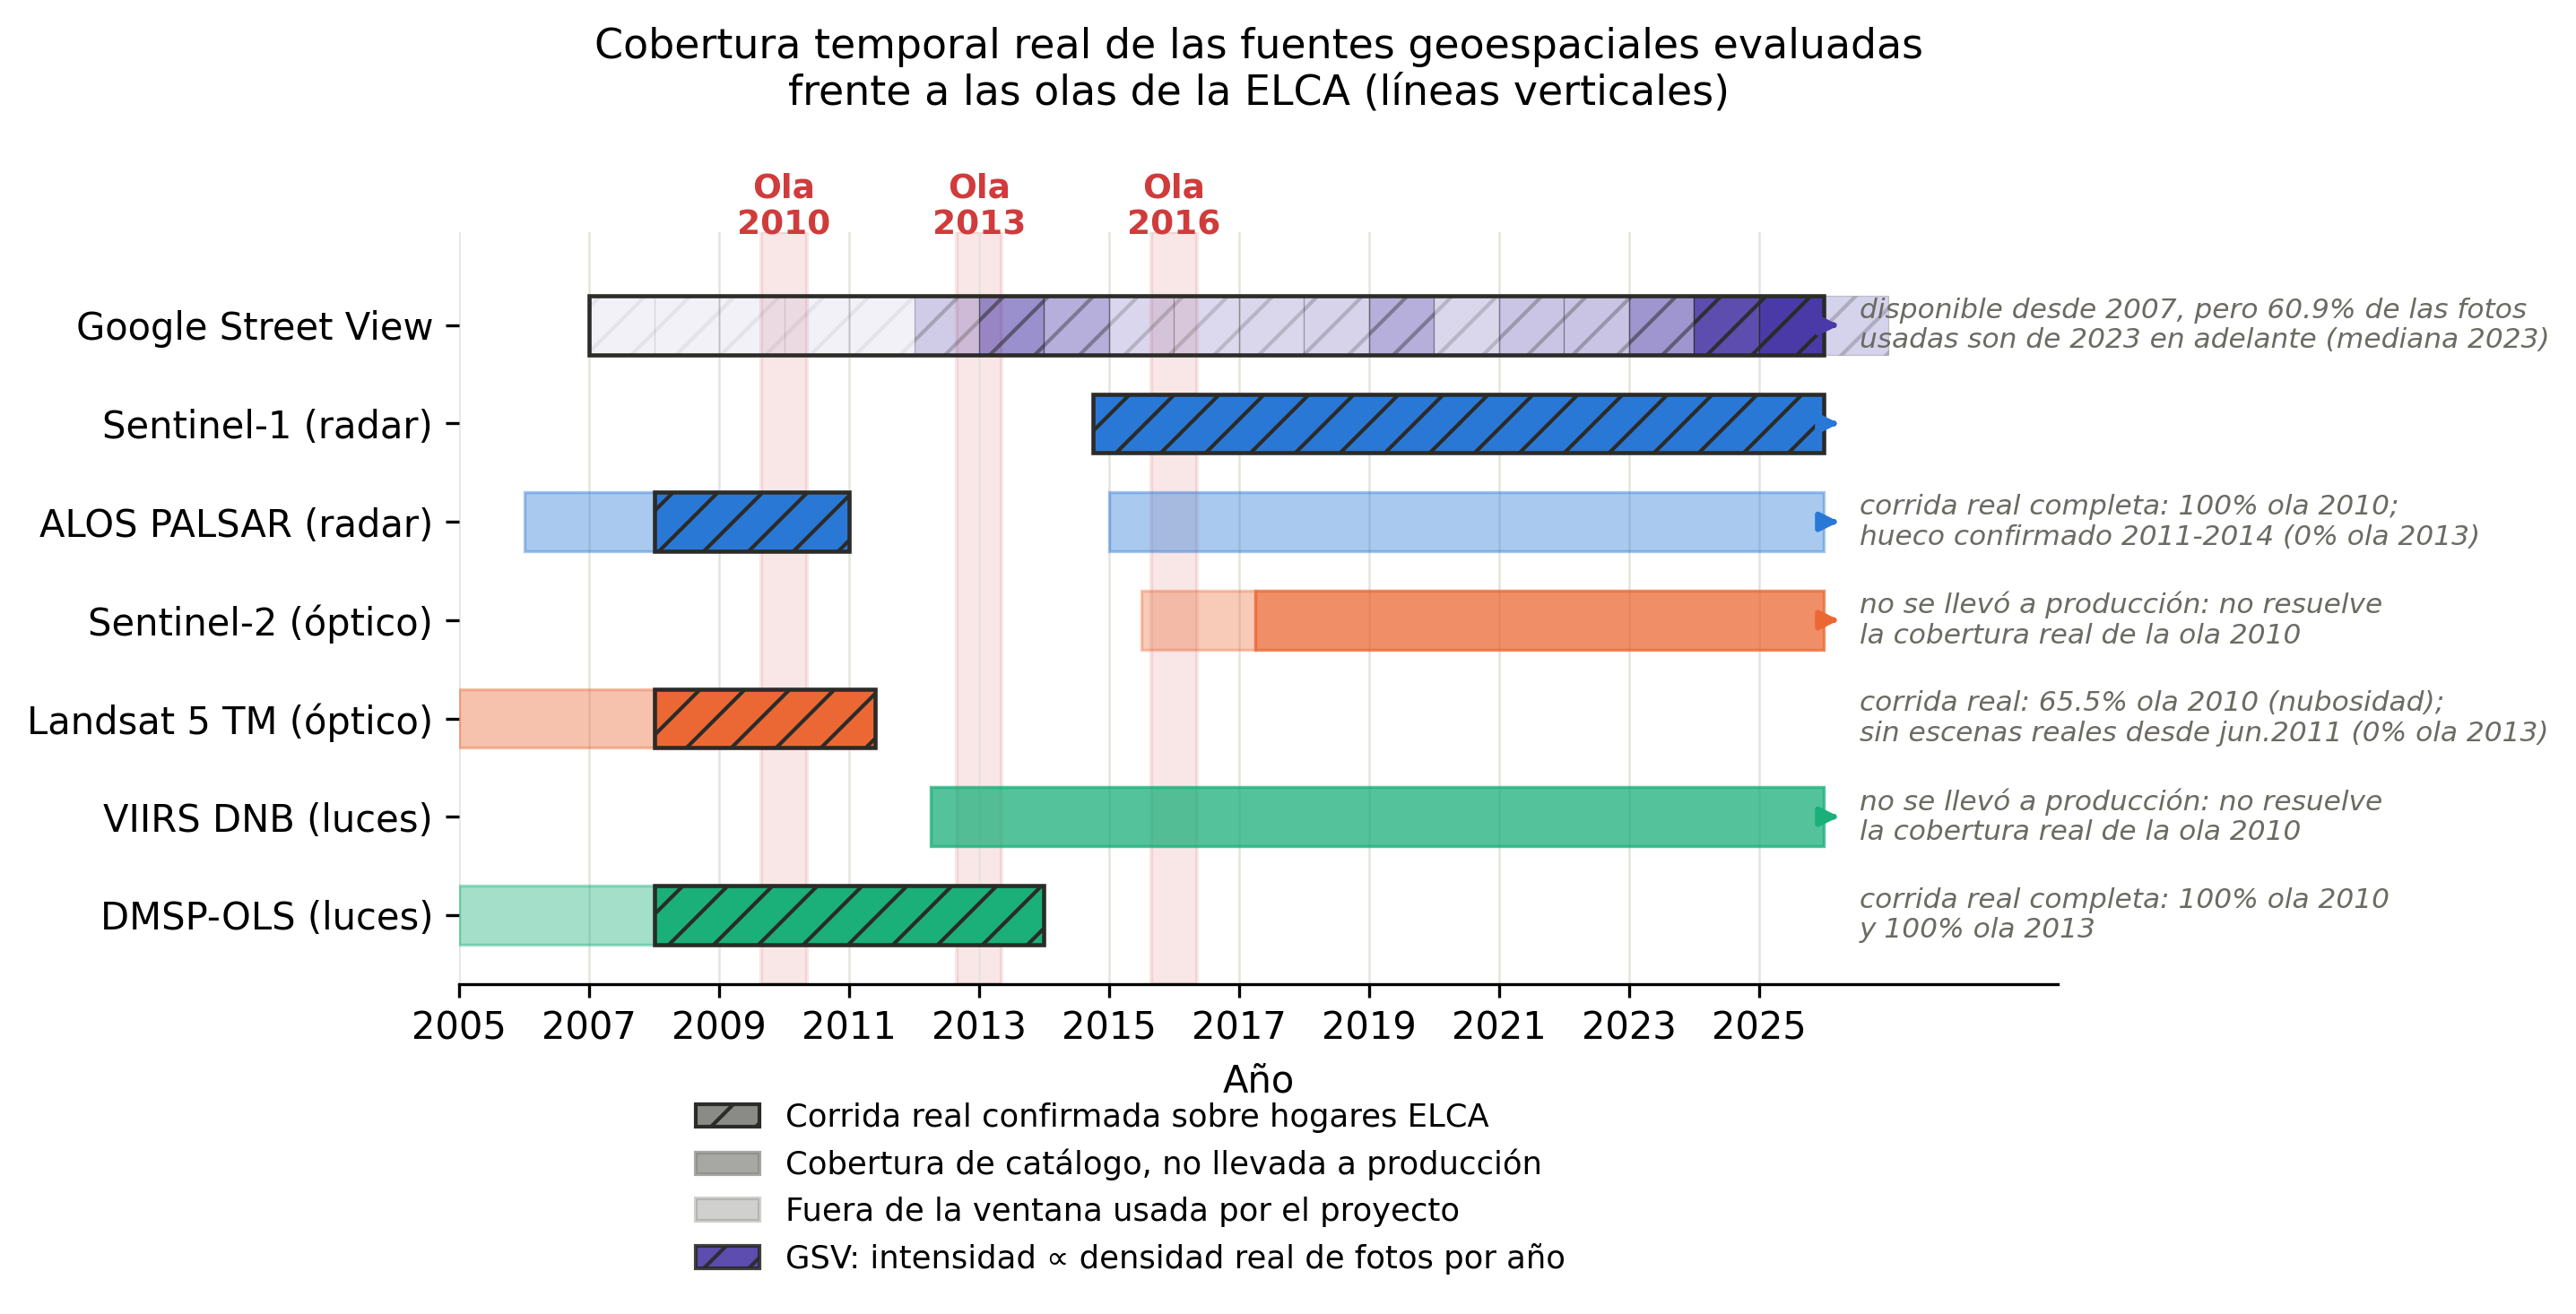
\includegraphics[width=0.95\textwidth]{figures/fig_cobertura_temporal_fuentes.png}
  \caption{Cobertura temporal real de cada fuente geoespacial evaluada,
  frente a las tres olas de la ELCA con coordenadas disponibles. El
  patrón diagonal indica corrida real y completa sobre
  hogares del estudio; el resto se revisó cobertura según catálogo. En la barra de GSV, la
  intensidad del color es proporcional a la densidad real de fotos por
  año —la gran mayoría de las fotos son de 2023 en adelante.}
  \label{fig:cobertura_temporal_fuentes}
\end{figure}

El resultado de la consulta de la información geoespacial, ya completa sobre las tres disponibles, es
asimétrico. DMSP-OLS cubre el 100\% de los hogares tanto en 2010 como en
2013; es la única de las
tres con esa cobertura completa en dos olas, lo que permite usarla
para la evaluación del poder predictivo en la
transición 2013$\to$2016. ALOS PALSAR cubre el 100\% de los hogares en
2010, pero tiene un hueco de información confirmado en el catálogo de JAXA entre 2011 y
2014 —no tiene ninguna cobertura de 2013—. Landsat 5 TM cubre solo 65.5\%
de los hogares en 2010 (6{,}269 de 9{,}573; del resto no se obtiene 
información por nubosidad persistente, una limitación del sensor
óptico) y, pese a que su fecha formal de salida (junio de 2013)
sugeriría cobertura parcial de esa ola, una consulta directa al catálogo
de Google Earth Engine confirmó que el sensor dejó de adquirir información
utilizable antes de esa fecha, no hay ninguna imagen real de Landsat 5
en 2012 ni en 2013, en ningún punto del planeta. Las tres se incorporan
al proyecto.

La Tabla~\ref{tab:variables_pedagogico} resume, para las tres fuentes
nuevas, el mecanismo físico de medición, el nombre de las variables
principales que se construyeron, y la interpretación 
que se les da en este estudio.

\begin{table}[H]
  \centering
  \caption{Qué mide cada fuente nueva, qué variables construye, y qué
  aproxima cada una.}
  \label{tab:variables_pedagogico}
  \small
  \begin{tabular}{lp{3.1cm}p{3.7cm}p{4.0cm}}
    \toprule
    \textbf{Fuente} & \textbf{Mecanismo físico} & \textbf{Variables (estado / ventana acum.)} & \textbf{Qué aproxima} \\
    \midrule
    DMSP-OLS &
    Radiancia visible nocturna captada por satélite (alumbrado público, vivienda, comercio) &
    Estado: nivel, log, saturación\newline
    Acumulada: media, tendencia, crecimiento (sobre \texttt{stable\_}\allowbreak\texttt{lights}) &
    Actividad económica y electrificación agregada del entorno (nivel); si el entorno se venía electrificando/densificando antes de la ola (ventana acumulada) \\
    \addlinespace
    ALOS PALSAR &
    Retrodispersión de radar en banda-L (HH, HV) sobre estructuras y vegetación &
    Estado: HH, HV (dB), razón HH/HV, índice normalizado\newline
    Acumulada: media, tendencia, crecimiento de cada una &
    Densidad y consolidación del entorno construido vs. vegetación (nivel); si la zona se venía densificando/deforestando antes de 2010 (ventana acumulada) \\
    \addlinespace
    Landsat 5 TM &
    Reflectancia óptica multiespectral (visible, infrarrojo cercano, infrarrojo de onda corta) &
    Estado: NDVI, NDBI, BSI, Tasseled Cap (10 índices)\newline
    Acumulada: media, tendencia, crecimiento de NDVI/NDBI/BSI/brillo &
    Cobertura vegetal y densidad de construcción del entorno inmediato (nivel); pérdida de vegetación o expansión de área construida antes de la ola (ventana acumulada) \\
    \bottomrule
  \end{tabular}
\end{table}


\subsection{Cobertura, atrición e inventario del panel}
\label{subsec:desc}

Los módulos de Hogar, Personas y
Choques cubren la totalidad del panel (27{,}932 observaciones) porque se
preguntan a todo hogar, sin condición previa. Comunidades y Niños no
llegan a 100\% porque comunidades se mide a un nivel de agregación distinto:
es comunidad$\times$ola, no hogar$\times$ola, por lo que representa un
92--96\% de cobertura. Esta cobertura incompleta refleja hogares cuya comunidad no
tuvo un registro correspondiente en esa ola; Niños, por
construcción, solo aplica a hogares con al menos un niño de 6 a 9 años en
el periodo, así que su 55.4\% de cobertura es exactamente la proporción
de hogares que cumplen esa condición. El detalle de candidatas auditadas,
variables usadas en el modelo y cobertura por módulo se reporta en la
Tabla~\ref{tab:cobertura_modulos} del Anexo~\ref{apx:cobertura_modulos}.

\subsubsection{Composición del panel y atrición}
\label{subsubsec:atricion}

En la ELCA existe pérdida de datos (atrición) que 
se caracteriza de la siguiente manera: el panel comienza con 9{,}853 hogares únicos en 2010 y se reduce
a 8{,}729 en 2013 y 8{,}086 en 2016 (Figura~\ref{fig:panel_atricion},
izquierda) —una atrición de 11.4\% entre 2010 y 2013, 11.4\% entre 2013 y
2016, y 17.9\% acumulada entre 2010 y 2016 (Figura~\ref{fig:panel_atricion},
derecha). Esta
pérdida no es aleatoria: se concentra en zonas urbanas (16.2\% de los
hogares urbanos de 2010 se pierden hacia 2013, frente a solo 5.8\% de los
rurales), lo opuesto a la intuición de que la atrición rural sería mayor
por dificultad de rastreo geográfico, probablemente porque la ELCA invierte
más esfuerzo de rastreo en hogares rurales. Por esta razón, en este estudio se utilizan técnicas de 
balanceo para compensar este sesgo.

\begin{figure}[H]
  \centering
  \includegraphics[width=0.48\textwidth]{../outputs/figures/eda_hogares/01_hogares_por_ola.png}
  \hfill
  \includegraphics[width=0.48\textwidth]{../outputs/figures/eda_hogares/03_attrition_tasas.png}
  \caption{Izquierda: hogares únicos por ola. Derecha: tasa de pérdida de
  hogares entre olas consecutivas y acumulada 2010--2016. Fuente: cálculos
  propios.}
  \label{fig:panel_atricion}
\end{figure}

Existe también un fenómeno de división de hogares. 511 hogares originales de 2010 se dividieron en
1{,}043 sub-hogares hacia 2013, y 679 hogares se dividieron en 1{,}411
sub-hogares hacia 2016 —típicamente porque un hijo formó su propio hogar
en la misma vivienda o predio—. Por eso el número de \emph{filas} del
panel hogar$\times$ola (9{,}853 / 9{,}261 / 8{,}818, ola 1/2/3) no coincide
con el número de hogares \emph{únicos} por ola: un sub-hogar nuevo aporta
una fila adicional sin ser, en sentido estricto, un hogar nuevo captado
por primera vez. Estos hogares divididos se excluyeron del análisis para no 
realizar ningún supuesto adicional.El número de personas cubiertas por el panel cae de
forma más pronunciada que el de hogares: 43{,}202 personas en 2010,
39{,}920 en 2013, 35{,}722 en 2016 (18.7\% de caída acumulada, por encima
del 17.9\% de hogares). Esto ocurre posiblemente porque los hogares perdidos tienden a ser, en
promedio, ligeramente más grandes que los que permanecen en el panel.

\subsubsection{Inventario temático de las variables finales}
\label{subsubsec:inventario}

El dataset consolidado que alimenta el modelo
(27{,}932 filas hogar$\times$ola) reúne 181 variables finales: 177 provienen de los
cinco módulos de la ELCA ya auditados en la
Tabla~\ref{tab:cobertura_modulos}, excluyendo de ese conteo
\texttt{consecutivo\_c}, que es la llave de unión al módulo Comunidades,
no una covariable, y las 4 restantes son las variables
geoespaciales. La
Personas (57) y Hogar/vivienda/activos (56) concentran más
de la mitad del inventario, consistente con que son los módulos que se
preguntan a todo hogar sin condición previa (Tabla~\ref{tab:cobertura_modulos}),
mientras que Comunidades (21), Choques (17), Niños (13) y Geoespacial (4)
son universos más acotados, ya sea por su nivel de agregación distinto
(Comunidades) o por aplicar solo a una submuestra o a una sola ola
(Niños, Geoespacial). De las 181, 159 (88\%) son numéricas continuas o de
conteo, 17 categóricas (principalmente características del jefe de hogar y
de la vivienda) y 5 booleanas (los indicadores de pobreza monetaria). El
desagregado por módulo y tipo de dato se muestra en la
Figura~\ref{fig:inventario_modulos} del Anexo~\ref{apx:cobertura_modulos}.

% ============================================================
% SECCIÓN 4 — ESTRATEGIA EMPÍRICA   TARGET: 6–7 páginas
% ============================================================
% Estructura interna recomendada:
%   4.1 Variable de resultado: matrices de transición — 1–1.5 pp.
%   4.2 Especificación de modelos — 2–2.5 pp.
%   4.3 Validación y métricas de desempeño — 1–1.5 pp.
%   4.4 Tratamiento del desbalance de clases — 0.5–1 p.
%   4.5 Importancia de variables e interpretabilidad — 0.5–1 p.
% ============================================================
\section{Estrategia empírica}
\label{sec:estrategia}

\subsection{Construcción de la variable de resultado y dinámica de transiciones}
\label{subsec:outcome}
\label{subsec:transiciones}

Este estudio sigue la metodología de \textcite{lopezCalva2011,lopezCalva2014}, 
a partir de la cual se construyen matrices de transición de pobreza monetaria e IPM, 
cruzando el estado de un hogar en el período inicial $t$ (filas), 
contra un periodo posterior $t+1$ (columnas). 
Esta comparación permite observar cómo evoluciona 
la situación económica de los hogares a lo largo del tiempo y generar
una taxonomía de cuatro categorías de acuerdo con la clasificación:
 \emph{nunca pobre}, \emph{siempre pobre}, \emph{entra en pobreza} y \emph{sale de pobreza}.
 
La pobreza monetaria se calcula a partir del cálculo del ingreso per
cápita del hogar y se compara contra la línea de pobreza (LP) oficial 
del DANE, específica por año y zona\footnote{Se usa la serie MESEP (línea base ENIG 2006--2007,
actualizada anualmente por IPC), la misma metodología para las tres olas
(2010, 2013 y 2016), lo que las hace comparables entre sí. Deliberadamente
no se usa la actualización metodológica ENPH 2016--2017 con la que el
DANE recalculó la serie 2012--2018, porque esa serie no cubre 2010 y
adoptarla habría introducido un quiebre metodológico justo entre las olas
que este estudio compara.}. El Índice de Pobreza Multidimensional (IPM)
y la construcción de la clasificación según el IPM se construye
siguiendo la metodología oficial del DANE \parencite{angulo2011}, como 
un proxy del índice Alkire-Foster de cinco dimensiones (educación; niñez y juventud;
trabajo; salud; vivienda y servicios públicos) y quince indicadores
ponderados (20\% por dimensión, peso igual entre
los indicadores de cada dimensión) y un punto de corte de pobreza de
33.3\% del puntaje ponderado.\footnote{Es un proxy porque cinco de los quince indicadores se
excluyen del puntaje final por huecos de cobertura irresolubles en la ola
2010 del panel: privación en primera infancia (no medible de forma
consistente en ninguna ola); inasistencia escolar y trabajo infantil
(\texttt{estudia}/\texttt{actividad\_ppal} en niños con 0.4\%--35.3\% de
cobertura en 2010, frente a ~100\% en 2013/2016); y empleo informal y
desempleo de larga duración (\texttt{actividad\_ppal} en adultos con
~20\% de cobertura en 2010, frente a 75--80\% en 2013/2016). Se calculan
y reportan para auditoría, pero no entran en la clasificación
\texttt{pobre\_ipm}. Quedan diez indicadores activos; la dimensión
Trabajo, que queda sin indicadores, redistribuye su 20\% entre las cuatro
dimensiones restantes (25\% cada una). El punto de corte de pobreza se
mantiene en 33.3\% del puntaje ponderado, independiente del número de
indicadores activos.} Ambas variables de resultado se describen en la 
Sección~\ref{sec:datos}--. El modelo predictivo de esta tesis
(Secciones~\ref{subsec:modelos} en adelante) usa solo una de las cuatro
celdas: restringido a hogares no pobres en $t$, que caen en pobreza en $t+1$, 
de acuerdo con la (Ecuación~\ref{eq:outcome}):

\begin{equation}
  \text{CaidaPobreza}_{i,t+1} =
  \begin{cases}
    1 & \text{si el hogar } i \text{ es pobre en } t+1 \\
    0 & \text{en cualquier otro caso}
  \end{cases}
  \label{eq:outcome}
\end{equation}

 A continuación se caracteriza las cuatro celdas completas. Se realizó un 
 análisis adicional de la incidencia agregada, FGT, y cinco ejercicios de 
 robustez de estas estimaciones, incluyendo la atrición del panel por 
 perfil de hogar y se documentan en el Apéndice~\ref{apx:transiciones_robustez}.


\begin{table}[H]
  \centering
  \caption{Matrices de transición de pobreza, monetaria por ingreso vs.
  IPM (\% de fila, panel emparejado 1 a 1). Estado inicial en filas,
  estado final en columnas.}
  \label{tab:matriz_transicion}
  \footnotesize
  \begin{tabular}{ll cc cc}
    \toprule
    & & \multicolumn{2}{c}{\textbf{Monetaria}} & \multicolumn{2}{c}{\textbf{IPM}} \\
    \textbf{Periodo} & \textbf{Estado inicial} & \textbf{No pobre} & \textbf{Pobre} & \textbf{No pobre} & \textbf{Pobre} \\
    \midrule
    \multirow{2}{*}{2010 $\rightarrow$ 2013} & No pobre & 76.6\% & 23.4\% & 87.9\% & 12.1\% \\
     & Pobre & 29.7\% & 70.3\% & 54.5\% & 45.5\% \\
    \addlinespace
    \multirow{2}{*}{2013 $\rightarrow$ 2016} & No pobre & 80.1\% & 19.9\% & 90.3\% & 9.7\% \\
     & Pobre & 38.2\% & 61.8\% & 52.3\% & 47.7\% \\
    \bottomrule
  \end{tabular}
  \begin{minipage}{0.95\textwidth}
    \vspace{4pt}
    \footnotesize \textit{Nota:} $n=8{,}218$ (2010$\to$2013) y $n=6{,}911$
    (2013$\to$2016) hogares con emparejamiento 1 a 1 -- idéntico universo para
    monetaria e IPM (mismo panel, solo cambia la clasificación de pobreza);
    excluye 511 (2010--2013) y 1{,}190 (2013--2016) casos de hogares que se
    dividieron entre olas. Fuente: cálculos propios con base en ELCA 2010,
    2013 y 2016.
  \end{minipage}
\end{table}

Bajo pobreza monetaria la persistencia es alta pero decrece: 70.3\% de los
pobres en 2010 seguían pobres en 2013, cae a 61.8\% entre 2013 y 2016 (la
salida condicional sube de 29.7\% a 38.2\%); la persistencia en la
no-pobreza mejora de 76.6\% a 80.1\%. Bajo IPM entrar es menos frecuente
(12.1\% y 9.7\%, frente a 23.4\% y 19.9\% en monetaria) pero también lo es
salir (45.5\% y 47.7\%). Estas diferencias son posiblemente consistentes 
con que el IPM mide privaciones estructurales que cambian más lento que 
el ingreso corriente en cualquiera de las dos direcciones. Las
Figuras~\ref{fig:sankey_2010_2013} y~\ref{fig:sankey_2013_2016} traducen
la matriz monetaria a flujos: en 2010--2013 dominan los \emph{siempre
pobres} (43.9\%) sobre los \emph{nunca pobres} (28.8\%); en 2013--2016 el
orden se invierte (37.0\% vs.\ 33.3\%), y en ambos periodos la salida
casi duplica la entrada, es decir, la pobreza monetaria se redujo de forma neta,
no solo se redistribuyó entre hogares.

\begin{figure}[H]
  \centering
  \begin{minipage}{0.49\textwidth}
    \centering
    \includegraphics[width=0.94\textwidth]{../outputs/figures/pobreza/sankey_transicion_pobreza_2010_2013.png}
    \caption{2010$\to$2013 ($n=8{,}218$).}
    \label{fig:sankey_2010_2013}
  \end{minipage}\hfill
  \begin{minipage}{0.49\textwidth}
    \centering
    \includegraphics[width=0.94\textwidth]{../outputs/figures/pobreza/sankey_transicion_pobreza_2013_2016.png}
    \caption{2013$\to$2016 ($n=6{,}911$).}
    \label{fig:sankey_2013_2016}
  \end{minipage}
  \caption*{Transición de pobreza monetaria por ingreso entre categorías
  de \textcite{lopezCalva2014}, panel emparejado 1 a 1.}
\end{figure}

Un último ejercicio (Tabla~\ref{tab:trayectorias_3olas}) sigue a los
mismos hogares no pobres en la ola base a lo largo de las tres olas para
distinguir, dentro de quienes \emph{entran} en pobreza, una entrada
transitoria de una persistente. Bajo pobreza monetaria, 24.1\% de los no
pobres en 2010 entra en pobreza en algún momento: 14.0 puntos salen de
nuevo antes de 2016 (``transitorio'') y 10.1 se quedan (``persistente'').
Bajo IPM la entrada total es menor (12.2\%) y se reparte parecido (8.2
transitoria, 4.0 persistente): en ambas definiciones, más de la mitad de
quienes entran en pobreza no quedan atrapados dentro de la ventana de
seis años observada.

\begin{table}[H]
  \centering
  \caption{Trayectorias a 3 olas (2010$\to$2013$\to$2016) de hogares
  NO pobres en 2010, panel emparejado 1 a 1, monetaria vs. IPM.}
  \label{tab:trayectorias_3olas}
  \footnotesize
  \begin{tabular}{lcccc}
    \toprule
    & \multicolumn{2}{c}{\textbf{Monetaria}} & \multicolumn{2}{c}{\textbf{IPM}} \\
    \textbf{Trayectoria} & \textbf{n} & \textbf{\%} & \textbf{n} & \textbf{\%} \\
    \midrule
    Nunca cae & 1{,}700 & 67.2\% & 4{,}381 & 81.2\% \\
    Cae tarde (solo en 2016) & 220 & 8.7\% & 357 & 6.6\% \\
    Entra y sale (transitorio) & 355 & 14.0\% & 445 & 8.2\% \\
    Entra y se queda (persistente) & 255 & 10.1\% & 214 & 4.0\% \\
    \bottomrule
  \end{tabular}
  \begin{minipage}{0.85\textwidth}
    \vspace{4pt}
    \footnotesize \textit{Nota:} $n$=2{,}530 hogares no pobres en 2010 bajo
    pobreza monetaria; $n$=5{,}397 bajo IPM (universos distintos porque
    no-pobre-monetaria y no-pobre-IPM en 2010 no son el mismo conjunto de
    hogares). \% sobre ese universo, sin ponderar (ver también
    \texttt{pct\_ponderado} en los CSV fuente). Fuente: cálculos propios,
    \texttt{outputs/tables/eda\_transicion\_covariables/trayectorias\_3olas\_\{monetaria,ipm\}.csv}
    (\texttt{src/02\_build/eda\_trayectorias\_3olas.py}), generados por
    \texttt{src/tabla\_trayectorias\_3olas.py}.
  \end{minipage}
\end{table}

\subsection{Selección de covariables para el perfil univariado}
\label{subsec:seleccion_perfil}

La Sección~\ref{subsec:caracterizacion_grupos} contrasta los cuatro
grupos de la matriz de transición sobre cerca de 185 covariables
candidatas de la encuesta. Describirlas todas sin ningún filtro sería
demasiado confuso: con muestras muy desiguales entre grupos (723 hogares
"entra" frente a 3.604 "siempre pobre" en 2010--2013), una simple
comparación de promedios o porcentajes no distingue una diferencia real
entre grupos de una que aparece por azar de qué hogares fueron
encuestados. Se necesita entonces una regla explícita para decidir qué
variables merecen contarse, y qué tan fuerte es esa diferencia --no solo
si existe--.

La regla, aplicada variable por variable, responde una pregunta simple:
¿qué tan bien predice el valor de esa única variable a cuál de los cuatro
grupos pertenece un hogar, en una escala de 0 (no ayuda nada) a 1 (los
distingue perfectamente)? Esa capacidad se mide con $\eta^2$ (variables
numéricas) o V de Cramér (categóricas) --la misma pregunta, la fórmula
adecuada según el tipo de dato--, en su versión corregida por sesgo
(ambas medidas exageran la asociación en muestras pequeñas, y "entra" es el
grupo más pequeño) y ponderada por los factores de expansión de la
encuesta. Una variable entra al perfil solo si esa medida supera 0.05 de
forma consistente en 300 remuestreos \emph{bootstrap} de los datos, no
solo en la muestra original: exige que la señal sea repetible, no una
casualidad de qué hogares puntuales aparecen en la encuesta. De las 185
candidatas, 53 (monetaria) y 36 (IPM) pasan el filtro. A diferencia de un
modelo predictivo, las variables que pasan no se colapsan aunque estén
correlacionadas entre sí: el objetivo aquí es describir, no evitar
redundancia, y cada variable retenida puede aportar información al perfil.

\subsection{Especificación de modelos}
\label{subsec:modelos}
La estrategia empírica se establece mediante la siguiente especificación 
de modelo:

% Ecuación del modelo base
\begin{equation}
  P\!\left(\text{CaidaPobreza}_{i,t+1} = 1 \mid X_{it}\right)
  = F\!\left(X_{it}\,\beta\right)
  \label{eq:modelo_base}
\end{equation}

\noindent donde $X_{it}$ es el vector de características del hogar $i$
observadas en el periodo $t$ (Sección~\ref{subsec:elco}) y $F(\cdot)$ es
la función que relaciona esas características con la probabilidad de
transición, aproximada de manera distinta según el algoritmo. Se estiman
y comparan cinco algoritmos, agrupados en dos familias según cómo tratan
las variables categóricas y los datos faltantes (Sección~\ref{subsec:desbalance}):

\begin{itemize}
  \item \textbf{Regresión logística regularizada (benchmark).} $F(\cdot)$
  es la función logística; los coeficientes $\beta$ se estiman
  penalizando su magnitud con una combinación de regularización L1 y L2
  (\emph{elastic net}), cuya fuerza ($C$) y mezcla ($l_1\_ratio$) se
  eligen por validación cruzada en vez de fijarse \emph{a priori} como
  Lasso o Ridge. Es el algoritmo designado como referencia por ser
  interpretable,
  y por servir de punto de comparación antes de
  justificar el uso de un modelo más complejo. Es también el más sensible
  a la multicolinealidad entre covariables --se evaluó explícitamente ese
  riesgo mediante un análisis de correlación de Pearson entre las 159
  variables numéricas del consolidado, con 35 pares por encima de
  $|r|=0.7$ (incluida una correlación fuerte de \texttt{dmsp\_stable\_lights}
  con \texttt{lp} y \texttt{n\_servicios\_publicos\_hogar}, retomada en la
  Sección~\ref{subsec:marginal}; detalle completo en el
  Apéndice~\ref{apx:correlacion})--: la regularización $\ell_1$/$\ell_2$
  mitiga, pero no elimina, la varianza inflada de coeficientes individuales
  cuando varias variables de un mismo grupo redundante entran juntas al
  modelo.
  \item \textbf{Random Forest.} Promedio de árboles de decisión
  entrenados sobre muestras \emph{bootstrap} independientes del conjunto
  de entrenamiento; captura no linealidades e interacciones entre
  covariables sin necesidad de especificarlas manualmente, con menor
  varianza que un árbol individual.
  \item \textbf{XGBoost, LightGBM y HistGradientBoosting.} Tres
  implementaciones de \emph{gradient boosting} de árboles. Este algoritmo
  es sobresaliente por su balance entre desempeño e interpretabilidad, 
  y uno de los más usados en la literatura de focalización de pobreza 
  \parencite{mcbride2018}--. Los
  tres manejan de forma nativa tanto los datos faltantes como las
  variables categóricas, sin necesidad de imputación ni de
  \emph{one-hot encoding} (Sección~\ref{subsec:desbalance}).
\end{itemize}

Para evaluar el aporte del nivel de ingreso/gasto del hogar
--el predictor más informativo bajo el enfoque de vulnerabilidad de
\textcite{chaudhuri2002}, que compara qué tan cerca está un hogar del
umbral de pobreza, se estima cada uno de los cinco algoritmos bajo dos
especificaciones de covariables: el \textbf{Modelo A} incluye el ingreso y
gasto per cápita real del hogar en el periodo base y la brecha frente a la
Línea de Pobreza (LP), de escala-invariante (se mantiene constante
a lo largo del tiempo); el \textbf{Modelo B}
excluye estas cuatro variables y usa exclusivamente covariables no
monetarias (ej. demografía, educación, activos, vivienda, choques,
comunidad). 

Finalmente, se establecieron dos variables objetivo para evaluar 
la robustez de los hallazgos: la transición hacia la 
pobreza monetaria y la transición 
hacia la pobreza multidimensional (IPM).

\subsection{Validación fuera de muestra y métricas}
\label{subsec:validacion}

La estimación usa las dos primeras olas de la ELCA como base de
entrenamiento (transición 2010 a 2013: covariables de 2010, resultado
observado en 2013) y la tercera ola como conjunto de prueba, completamente
independiente, para evaluar el desempeño predictivo fuera de muestra
(transición 2013 a 2016: covariables de 2013, resultado observado en
2016). Este recurso temporal hacia adelante replica el caso de uso
real de un sistema de focalización, solo existe la ola base al momento de
predecir, y es, siguiendo a \textcite{mcbride2018}, la validación más
exigente para un modelo de este tipo porque prueba generalización ante un
régimen económico distinto al de entrenamiento.

Dentro de ese periodo de entrenamiento (2010 a 2013) --nunca sobre el
conjunto de prueba-- cada algoritmo pasa por una búsqueda de
hiperparámetros: en vez de fijar a mano valores como la profundidad de los
árboles o la tasa de aprendizaje, \texttt{RandomizedSearchCV} propone 30
combinaciones aleatorias dentro de un rango razonable para cada
hiperparámetro (Sección~\ref{subsec:modelos}) y evalúa cada una con
validación cruzada estratificada de 10 particiones: el conjunto de
entrenamiento se divide en 10 bloques del mismo tamaño y manteniendo la
proporción de hogares que entran a la pobreza en cada uno
(\emph{estratificada}), se entrena 10 veces dejando un bloque distinto por
fuera cada vez y evaluando sobre ese bloque no visto, y se promedian las
10 evaluaciones. Ese promedio castiga a las combinaciones que memorizan
particularidades del conjunto de entrenamiento en vez de aprender un
patrón que generaliza, sin utilizar el conjunto de prueba, que solo se toca
una vez, al final, para evaluar el desempeño del modelo. Se eligen los 30 hiperparámetros por costo
computacional --evaluar más combinaciones exhaustivamente (\emph{grid
search}) sobre 5 algoritmos $\times$ 4 especificaciones $\times$ 3
estrategias de balanceo (Sección~\ref{subsec:desbalance}) y dos variables
objetivo, con validación cruzada de 10 particiones, hubiera requerido un
tiempo de cómputo prohibitivo, incluso con paralelización y
optimizaciones de preprocesamiento. La métrica que decide qué combinación
gana esa búsqueda es AUC-ROC. Para verificar que 30 iteraciones no se
quedan cortas, se extendió la búsqueda a 50 iteraciones para el caso más
ambiguo de la comparación de balanceo (HistGradientBoosting-A,
Sección~\ref{subsec:desbalance}): el mejor puntaje acumulado ya no mejora entre las
iteraciones 20 y 40 (0.7603 en ambas), y gana solo 0.0006 adicional hacia
la iteración 50 --evidencia de que la búsqueda con 30 iteraciones ya
opera cerca de su techo para este caso, no de que se haya interrumpido
prematuramente.

Un desbalance de clases pronunciado puede hacer que el AUC-ROC dé una
imagen optimista: premia una tasa \emph{relativa} baja de falsos
positivos, lo que puede esconder un número \emph{absoluto} alto de falsos
positivos cuando la clase positiva es escasa \parencite{davis2006,saito2015}.
Esto no invalida al AUC-ROC como medida de \emph{ranking} --su valor es
independiente del umbral de clasificación y no cambia mecánicamente con
la proporción de clases--, pero sí limita qué tan bien comunica, por sí
solo, la utilidad práctica del modelo para una política con cobertura
limitada. Por eso, además de AUC-ROC, se reporta \texttt{precision\_top10}
(Sección~\ref{subsec:marginal}): la precisión en el decil de mayor riesgo
no depende del balance de clases ni de un umbral de clasificación, y
responde directamente la pregunta relevante para un programa de
focalización real.

El desempeño se reporta mediante AUC-ROC como métrica principal, principalmente porque no
depende de un umbral de clasificación arbitrario (se evalúan múltiples umbrales), además, recall, precision y
F1 como métricas de referencia al umbral de clasificación elegido por F$_2$
(Sección~\ref{subsec:desbalance}), junto con la matriz de confusión
completa; F1 se sigue reportando por ser la referencia más estándar en la
literatura, aunque no es la métrica que decide dónde queda el umbral que se elige
mediante F$_2$. El foco del análisis está en comparar el desempeño relativo
entre los cinco algoritmos y entre las especificaciones A y B, más que en
declarar un único ``mejor'' modelo a partir de diferencias de AUC-ROC que,
como se documenta en la Sección~\ref{subsec:desempeno}, resultan pequeños
frente a la variabilidad esperable por aleatoriedad del ajuste.

\subsection{Tratamiento del desbalance de clases}
\label{subsec:desbalance}

La tasa de entrada a la pobreza en la muestra de entrenamiento es de
23.4\% (Tabla~\ref{tab:matriz_transicion}), un desbalance que
puede sesgar a los algoritmos hacia la clase mayoritaria. Se comparan tres
estrategias de tratamiento del desbalance para cada algoritmo:
reponderación de clases (\texttt{class\_weight="balanced"} o su
equivalente \texttt{scale\_pos\_weight} en XGBoost), ausencia de ajuste
(línea base), y sobremuestreo aleatorio de la clase minoritaria
(\texttt{RandomOverSampler}, aplicado únicamente dentro de cada partición
de entrenamiento de la validación cruzada, nunca contaminando la partición
de validación). No se usó SMOTE, que interpola sintéticamente entre
observaciones vecinas, porque no está bien definido cuando coexisten
variables categóricas y datos faltantes estructurales, a diferencia del
sobremuestreo aleatorio, que solo duplica filas existentes. La estrategia
que gana para cada algoritmo y especificación es la que maximiza el
AUC-ROC promedio en validación cruzada, no un criterio fijado \emph{a
priori}.

Esa selección, sin embargo, no siempre es robusta al azar del propio
particionado de validación cruzada: para HistGradientBoosting-A, repetir
la comparación de balanceo con 5 semillas distintas de
\texttt{StratifiedKFold} cambia la estrategia ganadora en 3 de 5 corridas --``balanced'' gana con
dos semillas, ``ninguno'' con otras dos, y \emph{oversampling} con la
restante--, con un AUC-CV que varía apenas en el tercer decimal entre
estrategias dentro de cada semilla (rango de 0.0013 a 0.0022). Esto no
invalida el procedimiento --la estrategia elegida para cada algoritmo en
el resto del documento es siempre la de la semilla base
(\texttt{RANDOM\_STATE=42}), fijada \emph{ex ante}, no elegida
\emph{ex post} entre semillas--, pero sí indica que, al menos para este
algoritmo y especificación, la diferencia entre estrategias de balanceo
está dentro del margen de ruido del particionado, no es una preferencia
robusta del algoritmo por una estrategia en particular.

Un hallazgo metodológico relevante de este ejercicio: en XGBoost y en
LightGBM (Modelo B), la estrategia ``sin ajuste'' ganó la comparación por
una diferencia de AUC-ROC frente a la reponderación de apenas 0.001
(estadísticamente indistinguible), pero el modelo resultante,
sin corregir el desbalance de clases, produjo probabilidades tan
comprimidas hacia valores bajos que casi ninguna observación cruzaba el
umbral convencional de 0.5 (recall de 3\%--4\% en XGBoost, con precision
superior a 60\%: el modelo ordenaba razonablemente bien los hogares por
riesgo, pero era inútil en la práctica al umbral estándar). Esto ilustra
que el umbral 0.5 es arbitrario cuando la clase positiva no es 50\% de la
muestra, y que distintas estrategias de balanceo calibran las
probabilidades de forma distinta, por lo que comparar recall/precision/F1
a un umbral fijo entre estrategias no es una comparación válida. La
solución adoptada fue elegir el umbral de clasificación de cada modelo por
validación cruzada, igual que los hiperparámetros: sobre las
probabilidades \emph{out-of-fold} (10 particiones) se evalúa una grilla de 
umbrales entre 0.02 y 0.98 y se
elige el que maximiza una métrica que combina recall y precision --el
AUC-ROC, que no depende de umbral, y sigue siendo el criterio que decide la
estrategia de balanceo y los hiperparámetros en el paso anterior; el
umbral solo determina cómo se reportan recall, precision y F1 una vez el
modelo ya está fijo.

La métrica elegida para esa búsqueda de umbral es F$_2$ (F-beta con
$\beta=2$) en vez del F1 convencional. F1 es la media armónica de recall y
precision con el mismo peso para ambos, una elección razonable cuando un
falso negativo (un hogar que sí cae en pobreza y el modelo no lo marca como
en riesgo) y un falso positivo (un hogar que el modelo marca como en riesgo y no
cae) son igual de costosos. En un sistema de focalización de política
social eso no es cierto: dejar sin detectar a un hogar que va a entrar en
pobreza es muy costoso socialmente --no recibe el apoyo que necesitaría--, es
un costo mucho mayor que incluir de más a un hogar que no cae, que en el peor caso implica un gasto
de focalización mal dirigido pero no la ausencia de una protección que se
necesita. F$_2$ formaliza esa prioridad ponderando el recall el doble
que la precision al elegir el umbral, de modo que el modelo se ajusta para
dejar pasar menos casos reales de entrada a la pobreza, a costa de marcar
como riesgo a más hogares que finalmente no caen.

Para los algoritmos sin soporte de datos faltantes (regresión
logística y Random Forest), la imputación de valores faltantes, que en
esta base de datos son mayoritariamente por la estructura de la encuesta, es decir, causados por
preguntas filtro del cuestionario (por ejemplo, el monto de una ayuda
recibida no se pregunta a quien respondió que no recibió ninguna)-- usa
sistemáticamente el valor 0 combinado con una columna
indicadora binaria de faltante por variable. Esta elección evita que la
mediana --calculada únicamente sobre quienes pasaron el filtro y
respondieron-- le asigne a los hogares excluidos por el filtro un valor
``típico'' que en realidad no tienen, y tiene además la propiedad de que,
en un modelo lineal, el relleno no aporta ninguna contribución a la
predicción más allá de la que capture el propio indicador de faltante. Las
variables categóricas se imputan con una categoría explícita ``Sin dato''
en vez de la moda, para no disfrazar la ausencia estructural como el valor
más común. XGBoost, LightGBM y HistGradientBoosting no requieren esta
imputación: manejan los datos faltantes de forma nativa en la partición de
los árboles, lo que convierte el propio patrón de \emph{missingness} en
una señal explotable por el modelo (por ejemplo, la ausencia de datos de
vacunación infantil ya codifica indirectamente que el hogar no tiene
hijos pequeños) en vez de forzar un supuesto de imputación potencialmente
sesgado.

\subsection{Importancia de variables e interpretabilidad}
\label{subsec:interpretabilidad}

Para cada modelo se reporta una medida de importancia de variables acorde
a su naturaleza: los coeficientes estandarizados (con signo) de la
regresión logística; la importancia por reducción de impureza
(\texttt{feature\_importances\_}) de Random Forest, XGBoost y LightGBM; y
la importancia por permutación (\emph{permutation importance}, AUC-ROC
sobre el conjunto de prueba, 10 repeticiones) de HistGradientBoosting, más
costosa computacionalmente pero más robusta a la correlación entre
covariables que la importancia basada en impureza. La comparación de estas
listas de variables más importantes entre el Modelo A y el Modelo B
(Sección~\ref{subsec:desempeno}) es la primera aproximación a la pregunta
de qué información no monetaria es más predictiva de la transición a la
pobreza, antes de la incorporación de las variables geoespaciales
(Sección~\ref{subsec:limitaciones}). Como estas medidas no comparten
unidad entre algoritmos (impureza vs.\ coeficiente estandarizado vs.\
caída de AUC-ROC), se complementan con valores SHAP (\emph{SHapley
Additive exPlanations}) para los cinco algoritmos sobre los Modelos A y
B, que sí son comparables en una misma escala --la contribución promedio,
en valor absoluto, de cada variable a la predicción de cada hogar-- y que
además satisfacen aditividad (la suma de los SHAP values de un hogar
reconstruye exactamente su predicción) y consistencia (si un modelo pasa
a depender más de una variable, su SHAP value nunca puede bajar). Los
resultados se presentan en la Sección~\ref{subsec:desempeno}.

\section{Resultados}
\label{sec:resultados}

A continuación se presentan los resultados en cinco partes, desde dos metodologías
distintas, un análisis descriptivo (univariado) y un análisis predictivo (multivariado). La
Sección~\ref{subsec:caracterizacion_grupos} es un análisis
\textbf{univariado e inicial}: perfila al hogar vulnerable --el que entra
en pobreza-- contra los otros tres grupos de la matriz de transición,
variable por variable (sin controlar por las demás
covariables), para las 53 (monetaria) y 36 (IPM) covariables que se hallaron como las 
más robustas para discriminar entre los grupos. Su función es exploratoria y 
descriptiva: construir la intuición sobre quién es el hogar vulnerable antes de imponerle cualquier
supuesto de modelo. La Sección~\ref{subsec:desempeno} cambia de
metodología --pasa a un enfoque \textbf{multivariado}-- y de objetivo:
ya no describe diferencias marginales entre grupos, sino que busca
\textbf{predecir} la vulnerabilidad a partir del conjunto de
covariables, con la mira puesta en generar insumos para una política
pública diferenciada (focalización de programas de prevención hacia
quienes el modelo señala en mayor riesgo, distinto de los programas de
alivio dirigidos a quien ya es pobre). Compara el desempeño fuera de
muestra de los cinco algoritmos bajo las especificaciones con y sin
ingreso/gasto del hogar. Es de aclarar, que la importancia de las variables 
puede variar según el algoritmo utilizado, la especificación del modelo y 
frente al análisis univariado. Las Secciones~\ref{subsec:marginal}
y~\ref{subsec:marginal_ipm} y~\ref{subsec:heterogeneidad} se mantienen en
el mismo objetivo de informar posibles insumos para la política pública, pero revisan la
utilidad metodológica de otras herramientas bajo ese mismo interés:
evalúan si agregar DMSP-OLS mejora esa predicción, bajo pobreza monetaria
e IPM respectivamente y por qué, y si ese efecto --nulo en promedio bajo
monetaria, pequeño bajo IPM-- es igual en la población o se concentra en
subgrupos específicos.

\subsection{Desempeño comparativo de modelos}
\label{subsec:desempeno}

Antes de comparar el desempeño de los cinco algoritmos, conviene fijar
brevemente qué mide cada métrica y cómo se relacionan entre sí. El
AUC-ROC resume la capacidad de un modelo para ordenar correctamente los
hogares por riesgo, sin depender de ningún umbral de clasificación --es
la métrica que compara algoritmos entre sí (Sección~\ref{subsec:validacion})--.
\emph{Recall} y \emph{precision}, en cambio, sí dependen del umbral
elegido: recall es la fracción de hogares que efectivamente entran en
pobreza y el modelo marca como riesgo (cuánta pobreza real se captura),
precision es la fracción de los hogares marcados que efectivamente entran
(cuánta de la alarma es acertada). Las tres no son independientes entre
sí: dado un AUC-ROC fijo, mover el umbral de clasificación permite subir
recall solo a costa de precision, y viceversa --el AUC-ROC actúa como un
techo que ninguna elección de umbral puede superar, solo desplazar el
punto donde se cae dentro de esa restricción--. Esta sección se organiza
en dos partes: primero el desempeño comparado de los cinco algoritmos, y
luego, apoyándose en esa restricción, un análisis de los errores de
inclusión y exclusión que resulta inevitable en cualquier instrumento de
focalización con ese techo de discriminación.

\subsubsection{Desempeño de los modelos}
\label{subsec:desempeno_modelos}

La Tabla~\ref{tab:desempeno_modelos} presenta el desempeño de los cinco
algoritmos bajo las dos especificaciones de covariables (Modelo A, con
ingreso/gasto; Modelo B, sin ellos), evaluado sobre el conjunto de prueba
completamente fuera de muestra (2013$\to$2016), con la estrategia de
balanceo de clases y el umbral de clasificación ya elegidos por validación
cruzada dentro del periodo de entrenamiento (Secciones~\ref{subsec:validacion}
y \ref{subsec:desbalance}).\footnote{Balanceo elegido por validación
cruzada: \emph{ninguno} (sin reponderar) en todos los casos, excepto
HistGradientBoosting y la regresión logística en el Modelo A, y Random
Forest y la regresión logística en el Modelo B, donde fue \emph{balanced}
(reponderación de clases).}

\begin{table}[H]
  \centering
  \caption{Desempeño de los cinco algoritmos en el conjunto de prueba
  (2013$\to$2016), promedio de 5 semillas. Prec.-top10: precisión en el
  10\% de hogares con mayor riesgo predicho.}
  \label{tab:desempeno_modelos}
  \footnotesize
  \setlength{\tabcolsep}{4pt}
  \begin{tabular}{llcccccc}
    \toprule
    \textbf{Algoritmo} & \textbf{Espec.} & \textbf{Umbral} & \textbf{AUC-ROC} & \textbf{Recall} & \textbf{Precision} & \textbf{Prec.-top10} & \textbf{F1} \\
    \midrule
    XGBoost                    & A & 0.11 & 0.767 & 0.949 & 0.264 & 0.505 & 0.413 \\
    Random Forest              & A & 0.14 & 0.766 & 0.926 & 0.277 & 0.486 & 0.426 \\
    HistGradientBoosting       & A & 0.32 & 0.763 & 0.909 & 0.283 & 0.512 & 0.432 \\
    LightGBM                   & A & 0.10 & 0.758 & 0.903 & 0.281 & 0.516 & 0.428 \\
    Logística regularizada     & A & 0.37 & 0.747 & 0.883 & 0.280 & 0.506 & 0.426 \\
    \addlinespace
    Random Forest              & B & 0.31 & 0.742 & 0.892 & 0.272 & 0.508 & 0.416 \\
    XGBoost                    & B & 0.13 & 0.742 & 0.940 & 0.250 & 0.495 & 0.395 \\
    Logística regularizada     & B & 0.35 & 0.739 & 0.890 & 0.270 & 0.500 & 0.414 \\
    HistGradientBoosting       & B & 0.14 & 0.735 & 0.879 & 0.275 & 0.494 & 0.418 \\
    LightGBM                   & B & 0.15 & 0.731 & 0.909 & 0.259 & 0.487 & 0.403 \\
    \bottomrule
  \end{tabular}
  \begin{minipage}{0.95\textwidth}
    \vspace{4pt}
    \footnotesize \textit{Nota:} umbral elegido por validación cruzada
    maximizando F$_2$ en cada semilla (Sección~\ref{subsec:desbalance}), no
    fijo en 0.5; se reporta el promedio de las 5 semillas. El umbral es
    considerablemente más bajo que en una búsqueda equivalente por F1 --al
    pesar el recall el doble, F$_2$ empuja el punto de corte hacia abajo
    para dejar pasar más casos de entrada a la pobreza, a costa de más
    falsos positivos (columna Recall, sistemáticamente sobre 0.88, frente a
    un F1 más moderado). Prec.-top10: precisión entre el 10\% de hogares
    que el modelo señala como de mayor riesgo, la cifra más relevante para
    un programa de focalización con capacidad fija (Sección~\ref{subsec:validacion}).
  \end{minipage}
\end{table}

Frente al desempeño de los modelos, se encontraron dos hallazgos a partir de las diferencias
puntuales entre los desempeños de los algoritmos y las especificaciones (Tabla~\ref{tab:desempeno_modelos}).
\textbf{Primero,} el algoritmo elegido
no cambia el poder de discriminación de los vulnerables (AUC-ROC 0.731--0.767 en los cinco).
Bajo IPM el mismo techo aparece, en un rango de AUC-ROC igual de estrecho (0.725--0.747; Tabla~\ref{tab:desempeno_modelos_ipm},
Apéndice~\ref{apx:desempeno_ipm}).
Un AUC-ROC de 0.75 significa que, si se toma al azar un hogar que entra en pobreza y uno que no,
el modelo correctamente asigna mayor riesgo al primero solo 3 de cada 4 veces.
Esto es consistente con la literatura sobre predicción de pobreza
--AUC-ROC de 0.70--0.80 en \textcite{chaudhuri2002}, 0.73--0.77 en \textcite{mcbride2018}--.

\textbf{Segundo,} la capacidad de identificar vulnerables apenas cambia
si se excluyen las variables de ingreso/gasto del hogar de las
covariables que se utilizan en los modelos. La ganancia
de incluir esa información, que valga mencionar es la más cara de levantar mediante encuesta, 
y la menos confiable, es marginal (brecha de AUC de 0.008 a 0.028 entre
el Modelo A y B, mucho menor de lo que predeciría un enfoque de
vulnerabilidad puramente monetario, \textcite{chaudhuri2002}). Esto no
implica que el ingreso no importe, anteriormente se estableció que es de las variables
que más separa a los cuatro grupos de la matriz de transición (Sección~
\ref{subsec:caracterizacion_grupos})--, sino que su contenido informativo
ya está sustancialmente capturado por otras variables del núcleo del
perfil (riqueza, educación, bienes durables; Hallazgo 4,
Sección~\ref{subsec:caracterizacion_grupos}). Bajo IPM la brecha es aún
menor, y para Random Forest y XGBoost es negativa --el Modelo B (sin ingreso/gasto) supera al
A--, lo que descarta que la pequeña brecha en la capacidad discriminante 
de los modelos bajo la definición de pobreza monetaria se deba a la
relación mecánica entre ingreso y la definición de pobreza. La
implicación práctica sigue la misma lógica que sustenta focalizar con
proxies observables del ingreso en vez de medirlo directamente
\parencite{mcbride2018}: un instrumento más barato, sin ingreso/gasto
detallado, rendiría casi lo mismo.

\subsubsection{Análisis de los errores de inclusión y exclusión}
\label{subsec:errores_inclusion}

Aunque el poder de discriminación (AUC-ROC) es similar entre los cinco
algoritmos (Sección~\ref{subsec:desempeno_modelos}), el algoritmo y la
estrategia de elección del umbral sí determinan cuánta capacidad de
cobertura necesita un eventual programa social que focalice vulnerables
para no perder casos reales. En este estudio se encontró que ese costo,
con cualquier algoritmo, ronda entre los 3--4 hogares atendidos por cada
hogar que realmente lo necesitaba (Tabla~\ref{tab:matriz_confusion_a}): de
los hogares que efectivamente no entran en pobreza, HistGradientBoosting
identifica correctamente al 40\%, mientras XGBoost solo al 26\%. En
términos de las métricas de la Tabla~\ref{tab:desempeno_modelos}, esto
corresponde a un recall alto (0.88--0.95: casi todos los hogares que
efectivamente caen quedan marcados) pero una precisión baja (0.25--0.28:
solo uno de cada 4 marcados efectivamente cae); la precisión en el 10\%
de mayor riesgo (Prec.-top10, 0.49--0.52) casi duplica la precisión al
umbral completo, lo que sugiere que concentrar la atención en ese decil
sería una estrategia de focalización más eficiente que usar el umbral de
clasificación completo. El comportamiento de recall y precision obedece
no solo al modelo, sino en parte también a la decisión de diseño: el
umbral elegido por F$_2$, que pone el doble del peso en la importancia de
los falsos positivos que en los falsos negativos, determina dónde se cae
(vulnerable o no vulnerable) dentro del techo que impone el AUC. Lo que sí
es una restricción, que ninguna combinación de modelo y umbral pueden
resolver, es que con un AUC-ROC de 0.75 no es posible lograr recall y
precision altos simultáneamente. Este intercambio es el mismo que la
literatura de focalización de programas sociales llama errores de
inclusión y de exclusión (\emph{Type E} y \emph{Type F},
\textcite{cornia1993}): para un instrumento de focalización dado, reducir
uno necesariamente aumenta el otro; solo un instrumento con mayor poder de
discriminación --no un umbral distinto-- puede mover esa frontera.

\begin{table}[H]
  \centering
  \caption{Matriz de confusión, Modelo A, holdout temporal (test
  2013$\to$2016, semilla 42), pobreza monetaria ($n=3{,}191$) e
  IPM ($n=5{,}571$). VN/FP/FN/VP: hogares verdadero negativo, falso
  positivo, falso negativo y verdadero positivo, al umbral de
  clasificación de las Tablas~\ref{tab:desempeno_modelos} y
  \ref{tab:desempeno_modelos_ipm} respectivamente.}
  \label{tab:matriz_confusion_a}
  \footnotesize
  \setlength{\tabcolsep}{4pt}
  \begin{tabular}{lcccccccc}
    \toprule
     & \multicolumn{4}{c}{\textbf{Monetaria}} & \multicolumn{4}{c}{\textbf{IPM}} \\
    \cmidrule(lr){2-5} \cmidrule(lr){6-9}
    \textbf{Algoritmo} & \textbf{VP} & \textbf{FP} & \textbf{FN} & \textbf{VN} & \textbf{VP} & \textbf{FP} & \textbf{FN} & \textbf{VN} \\
    \midrule
    XGBoost                  & 617 & 1888 & 18 & 668 & 491 & 3297 & 51 & 1732 \\
    Random Forest            & 594 & 1572 & 41 & 984 & 343 & 1493 & 199 & 3536 \\
    HistGradientBoosting     & 584 & 1532 & 51 & 1024 & 301 & 1124 & 241 & 3905 \\
    LightGBM                 & 561 & 1354 & 74 & 1202 & 415 & 2052 & 127 & 2977 \\
    Logística regularizada   & 561 & 1444 & 74 & 1112 & 379 & 1862 & 163 & 3167 \\
    \bottomrule
  \end{tabular}
\end{table}


Se caracterizaron los falsos
positivos (Modelo A, HistGradientBoosting y XGBoost) comparándolos, en
las 22 variables del núcleo de importancia multivariada
(Sección~\ref{subsec:determinantes}), contra los verdaderos negativos
--hogares que en la realidad tampoco cayeron en pobreza, pero que el
modelo sí acertó en no marcar--: aislar esta comparación, en vez de
contrastar contra los verdaderos positivos, evita mezclar la pregunta de
``qué dispara la alarma del modelo'' con la de ``qué tan parecidos son a
quien sí cae''. Los falsos positivos ($n=1{,}464$ en HistGradientBoosting,
$1{,}695$ en XGBoost) resultan sistemáticamente más parecidos a un hogar
vulnerable que los verdaderos negativos ($n=1{,}092$ y $861$
respectivamente) en 18 de las 20 variables numéricas del núcleo: menos
riqueza, menos bienes durables, menor nivel educativo, menos servicios
públicos, menor estrato, más hacinamiento --no son errores aleatorios del
modelo, son hogares genuinamente al borde de la línea de pobreza. Los
valores SHAP confirman, además, que estas mismas variables --no otras
correlacionadas de fondo-- son las que efectivamente empujan la
predicción hacia ``riesgo'': para HistGradientBoosting, la brecha más
grande entre falsos positivos y verdaderos negativos está en
\texttt{riqueza\_pca\_hogar} y \texttt{nivel\_educ\_max\_hogar}; para
XGBoost, en \texttt{ingreso\_percapita\_hogar\_real}
(\emph{diferencia} de SHAP de 0.44, el doble que la segunda variable) y
\texttt{brecha\_lp\_ingreso} --consistente con que cada algoritmo
distribuye el mismo núcleo de forma distinta (Sección~\ref{subsec:determinantes}).

Queda una pregunta: si los falsos positivos se ven igual de vulnerables
que los verdaderos positivos a ojos del modelo, ¿qué distingue a quien
efectivamente cae de quien no? Comparando choques reportados en la ola de
destino (2016, posteriores al momento de la predicción y por tanto no
usados por el modelo) entre verdaderos positivos y falsos positivos, los
primeros vivieron sistemáticamente más choques durante esa ventana: 3.1
choques en promedio frente a 2.2 (ambos algoritmos), y 81--82\% tuvo al
menos un choque frente a 71--72\% de los falsos positivos --consistente
con el enfoque de vulnerabilidad de \textcite{chaudhuri2002}: el modelo
identifica correctamente al hogar en el margen, pero quién realiza el
riesgo depende de una exposición a choques que ningún dato de encuesta
disponible al momento de la predicción puede anticipar.

\subsection{Determinantes de la vulnerabilidad: perfil e importancia de variables}
\label{subsec:determinantes}

Esta sección aborda los determinantes de la vulnerabilidad a la pobreza
desde dos perspectivas complementarias: el perfil univariado de los
hogares que entran en pobreza --comparándolos con los otros tres grupos
de la matriz de transición-- y la importancia de esas mismas variables
una vez se controla por el resto, dentro de los cinco algoritmos de la
Sección~\ref{subsec:desempeno}.

\subsubsection{Perfil univariado de los hogares vulnerables}
\label{subsec:caracterizacion_grupos}

Esta sección perfila los hogares que \textbf{entran en pobreza} entre 2010
y 2013 --no pobres en la ola inicial, pobres en la siguiente-- contra los
otros tres grupos de la matriz de transición
(Sección~\ref{subsec:transiciones}), sobre las 53 covariables que
distinguen de forma confiable a los cuatro grupos entre sí (criterio de
selección en la Sección~\ref{subsec:seleccion_perfil}),\footnote{40 de 53
superan 0.10; las 13 restantes cumplen efecto$>$0.05 y robustez en
\emph{ambas} transiciones por separado. Las 40 originales no se
sometieron a ese chequeo: 2 (\texttt{n\_ninos\_12},
\texttt{razon\_dependencia\_demografica}) caen bajo 0.10 en
2013$\to$2016 (0.105$\to$0.084 y 0.104$\to$0.088), aunque siguen
robustas.} sin colapsar las correlacionadas entre sí, en una sola tabla
consolidada (Tabla~\ref{tab:perfil_consolidada}).

Hay cuatro hallazgos principales de este análisis. \textbf{Primero,} el hogar
vulnerable se parece mucho más al que \emph{acaba de salir} de la pobreza
que al que nunca fue pobre o al que nunca sale de ella: de las 53
variables, 47 lo ubican numéricamente más cerca de ``sale de la pobreza''
que de ``nunca pobre'' (en promedio, cerca de cuatro veces más cerca) --
Tabla~\ref{tab:perfil_consolidada}. El patrón se repite, y se refuerza, en
la transición 2013$\to$2016 (49 de 53 variables más cerca de ``sale''): no
depende de una sola ola del panel. Tampoco depende de cómo se mida la
pobreza: el mismo ejercicio repetido bajo pobreza multidimensional (IPM,
36 variables robustas bajo el mismo criterio de la
Sección~\ref{subsec:seleccion_perfil}, Apéndice~\ref{apx:perfil_ipm})
confirma el mismo contraste (sale vs.\ nunca) en 29 de 36 variables en
2010$\to$2013 y 31 de 35 en 2013$\to$2016 -- el patrón es robusto tanto a
la ola como a la definición de pobreza. Esto es consistente con pensar
``entra'' y ``sale'' como las dos caras de
una misma frontera --hogares que cruzan la línea de pobreza en direcciones
opuestas, con un perfil similar por estar ambos cerca de ese umbral--, y
no como dos tipos de hogar distintos.
\textbf{Segundo,} cuatro variables (marcadas $^\dagger$ en la tabla) rompen ese patrón, es decir,
diferencian mejor a los hogares vulnerables de los demás grupos, todas en la
misma dirección --el hogar vulnerable queda en el extremo \emph{más
favorable}, no en el segundo peor--. La más importante es la \emph{formalidad
laboral del jefe}, la señal que convencionalmente se usaría para descartar
riesgo: 62.3\% de los jefes de hogar vulnerables son asalariados, más que
quien sale (52.2\%) y más que quien nunca cae (57.9\%). En 2013$\to$2016
esa ventaja frente a quien sale se mantiene (52.3\% frente a 46.9\%), pero
deja de superar a quien nunca cae (55.3\%). Las otras tres son
menores pero van en la misma dirección: \emph{deuda informal} (26.0\% frente a
22.7\% de los que salen), \emph{niños al cuidado de terceros} (98.9\% frente a 98.2\% de los que nunca son pobres) y
\emph{transporte público comunitario} (79.2\% frente a 78.2\% de los que nunca son pobres).
Estas tres no se sostienen en 2013$\to$2016: el vulnerable vuelve al orden
esperado, entre ``sale'' y ``siempre pobre'', en las tres --consistente
con que su efecto (0.051--0.058) apenas superaba el umbral de robustez,
un orden de magnitud por debajo del de formalidad laboral (0.393). Si una política
de focalización usara solo la formalidad laboral del jefe en 2010, habría
clasificado a los hogares vulnerables como los \emph{menos} necesitados de
los cuatro grupos --el ejemplo más concreto de por qué un estado
socioeconómico observado no revela el riesgo futuro de un hogar, y en el
caso del empleo formal, activamente lo oculta.

{\footnotesize\setlength{\tabcolsep}{4pt}
\begin{longtable}{p{0.40\textwidth}rrrr}
  \caption{Perfil por grupo de transición, pobreza monetaria (2010$\to$2013), las 53 variables robustas. $^{\dagger}$variable donde el hogar vulnerable no queda entre ``sale'' y ``siempre pobre''/``nunca pobre'' como el resto (ver texto).}\label{tab:perfil_consolidada}\\
    \toprule
    \textbf{Variable} & \textbf{Siempre} & \textbf{Sale} & \textbf{Entra} & \textbf{Nunca} \\
    \midrule
    \endfirsthead
    \multicolumn{5}{l}{\footnotesize \textit{(Cuadro~\ref{tab:perfil_consolidada}, continuación)}} \\
    \toprule
    \textbf{Variable} & \textbf{Siempre} & \textbf{Sale} & \textbf{Entra} & \textbf{Nunca} \\
    \midrule
    \endhead
    \bottomrule
    \multicolumn{5}{r}{\footnotesize \textit{continúa en la página siguiente}} \\
    \endfoot
    \bottomrule
    \endlastfoot
    \multicolumn{5}{l}{\textit{Educación y empleo del jefe}} \\
    \quad Educación del jefe: Básica primaria (1 a 5) & 59\% & 49\% & 47\% & 25\% \\
    \quad Ocupación del jefe: Asalariado$^{\dagger}$ & 34\% & 52\% & 62\% & 58\% \\
    \quad Consiguió trabajo: Pidiendo ayuda a familiares, amigos o colegas & 66\% & 69\% & 62\% & 54\% \\
    \quad Registro mercantil del jefe: No lo necesita & 63\% & 49\% & 42\% & 45\% \\
    \quad Negocio del jefe: De 20 a 49 personas & 9\% & 16\% & 22\% & 25\% \\
    \quad Máx. nivel educativo del hogar & 2.28 & 2.79 & 2.79 & 4.22 \\
    \quad Cotización a pensión (hogar) & 5\% & 16\% & 18\% & 38\% \\
    \quad Nivel educativo del jefe (ordinal) & 2.02 & 2.54 & 2.56 & 3.72 \\
    \quad Etnia del jefe: Indígena & 12\% & 6\% & 6\% & 4\% \\
    \quad Jefe cotiza a pensión & 6\% & 21\% & 24\% & 43\% \\
    \quad Estado civil del jefe: En unión libre & 46\% & 39\% & 43\% & 33\% \\
    \quad Afiliación a pensión (hogar) & 27\% & 51\% & 48\% & 57\% \\
    \quad Afiliación a salud laboral (hogar) & 33\% & 55\% & 58\% & 62\% \\
    \quad Jefe afiliado a salud laboral & 35\% & 53\% & 61\% & 64\% \\
    \quad Jefe afiliado a pensión & 29\% & 49\% & 51\% & 58\% \\
    \multicolumn{5}{l}{\textit{Vivienda: materiales y servicios}} \\
    \quad Material de piso: Baldosa, vinilo, tableta o ladrillo & 14\% & 31\% & 35\% & 59\% \\
    \quad Combustible de cocina: Leña, madera, carbón de leña & 64\% & 43\% & 32\% & 12\% \\
    \quad Servicio sanitario: Inodoro conectado a alcantarillado & 26\% & 47\% & 55\% & 79\% \\
    \quad Recolección de basura: La recogen los servicios de aseo & 31\% & 49\% & 57\% & 80\% \\
    \quad Obtención de agua: Acueducto público & 31\% & 49\% & 58\% & 79\% \\
    \quad Tipo de vivienda: Apartamento & 8\% & 18\% & 20\% & 38\% \\
    \quad Material de paredes: Bloque, ladrillo, piedra, madera pulida & 59\% & 75\% & 81\% & 91\% \\
    \quad Tenencia de vivienda: En usufructo u otro tipo de tenencia & 33\% & 24\% & 28\% & 15\% \\
    \quad Financió la vivienda con crédito formal & 13\% & 26\% & 22\% & 43\% \\
    \quad Tiene escritura de la vivienda & 67\% & 81\% & 80\% & 90\% \\
    \multicolumn{5}{l}{\textit{Zona de residencia}} \\
    \quad Vive en zona rural & 69\% & 52\% & 45\% & 21\% \\
    \multicolumn{5}{l}{\textit{Geoespacial}} \\
    \quad Iluminación nocturna (DMSP) & 21.6 & 32.6 & 36.4 & 50.1 \\
    \multicolumn{5}{l}{\textit{Activos del hogar}} \\
    \quad N.\textsuperscript{o} de bienes durables & 4.58 & 6.00 & 6.30 & 9.10 \\
    \quad N.\textsuperscript{o} de servicios públicos & 2.50 & 3.30 & 3.65 & 4.80 \\
    \quad Estrato (verificado) & 1.59 & 2.06 & 2.07 & 2.63 \\
    \quad Índice de riqueza (PCA) & -0.83 & -0.02 & 0.21 & 1.06 \\
    \quad Estrato (autorreportado) & 1.60 & 2.07 & 2.05 & 2.58 \\
    \quad Tiene internet en el hogar & 8\% & 16\% & 13\% & 46\% \\
    \quad N.\textsuperscript{o} de activos financieros & 0.10 & 0.42 & 0.45 & 0.86 \\
    \quad Tiene vehículo & 17\% & 25\% & 23\% & 40\% \\
    \multicolumn{5}{l}{\textit{Vivienda: hacinamiento}} \\
    \quad Valor del arriendo pagado & 144k & 226k & 240k & 354k \\
    \quad Personas por cuarto & 2.13 & 1.65 & 1.49 & 1.11 \\
    \quad Personas por dormitorio & 2.77 & 2.25 & 2.09 & 1.74 \\
    \multicolumn{5}{l}{\textit{Programas sociales y deuda}} \\
    \quad Beneficiario de Familias en Acción & 53\% & 29\% & 23\% & 7\% \\
    \quad N.\textsuperscript{o} de programas sociales & 0.73 & 0.42 & 0.34 & 0.17 \\
    \quad Beneficiario de algún programa social & 60\% & 37\% & 31\% & 15\% \\
    \quad Tiene deuda informal$^{\dagger}$ & 32\% & 23\% & 26\% & 9\% \\
    \quad Tiene deuda formal & 65\% & 75\% & 73\% & 88\% \\
    \multicolumn{5}{l}{\textit{Composición del hogar}} \\
    \quad N.\textsuperscript{o} de niños en el hogar & 1.45 & 0.92 & 0.79 & 0.57 \\
    \quad Razón de dependencia demográfica & 0.93 & 0.67 & 0.56 & 0.43 \\
    \quad Niños al cuidado de terceros$^{\dagger}$ & 86\% & 94\% & 99\% & 98\% \\
    \quad Niños con apoyo alimentario escolar & 81\% & 72\% & 70\% & 54\% \\
    \multicolumn{5}{l}{\textit{Comunidad}} \\
    \quad N.\textsuperscript{o} de espacios públicos en la comunidad & 1.57 & 1.98 & 2.13 & 2.32 \\
    \quad Comunidad con transporte público$^{\dagger}$ & 55\% & 75\% & 79\% & 78\% \\
    \multicolumn{5}{l}{\textit{Ingreso y gasto}} \\
    \quad Ingreso (veces la línea de pobreza) & 0.42 & 0.55 & 1.58 & 3.26 \\
    \quad Ingreso per cápita & 65k & 93k & 269k & 633k \\
    \quad Gasto per cápita & 154k & 210k & 247k & 662k \\
    \quad Gasto (veces la línea de pobreza) & 0.99 & 1.26 & 1.45 & 3.36 \\
\end{longtable}}


\textbf{Tercero,} y no visible en el promedio agregado: el grupo ``entra
en pobreza'' no es un solo tipo de hogar, sino dos trayectorias distintas
que el análisis de dos olas (2010$\to$2013) no alcanza a distinguir.
Siguiendo a esos mismos 723 hogares que entran a probreza - los vulnerables - 
hasta la tercera ola (610 con dato en
2016), se pueden separar según qué pasa después: \emph{pobre transitorio} --vuelve a
salir antes de 2016-- (355 hogares, 58\%) y \emph{pobre persistente} --sigue
pobre en 2016-- (255 hogares, 42\%; Tabla~\ref{tab:perfil_split_trayectoria}).
En ambos subgrupos se mantiene el patrón del primer hallazgo: transitorio
se parece más a ``sale'' que a ``nunca cae'' en 39 de 53 variables, y
persistente en 44 de 53. Pero el promedio de ``entra'' esconde un
gradiente que solo aparece al separarlos: "pobre persistente" se acerca al
extremo ``siempre pobre'' en 11 de esas 53 variables, frente a solo 2 en
"pobre transitorio" --. Es decir, dentro de quienes entran a pobreza, quien va a quedar atrapados ya se
parece un poco más al hogar crónicamente pobre, aunque el patrón
dominante siga siendo el de la frontera con ``sale''--. Al revisar las variables que caracterizan
a estos grupos, el caso más claro
es la \emph{deuda informal}: el promedio de ``entra'' (26.0\%) esconde que
pobre transitorio (17.3\%) queda por \emph{debajo} incluso de ``sale''
(22.7\%), mientras pobre persistente (41.9\%) supera a los cuatro grupos,
incluido ``siempre pobre'' (31.6\%) --separa, dentro del propio grupo
vulnerable, a quien va a recuperarse rápido de quien va a quedar
atrapado--. Este patrón no es exclusivo de la deuda: \emph{cotizar a pensión} y
el \emph{acceso a deuda formal} muestran la misma divergencia
(Tabla~\ref{tab:perfil_split_trayectoria}) --la misma frontera de
formalidad laboral y financiera que separa a ``entra'' de ``sale'' en el
Hallazgo 2 reaparece dentro de ``entra''(los vulnerables) para separar a quien se
recupera (pobre transitorio) de quien queda atrapado (pobre persistente).
Este gradiente también se confirma bajo IPM: pobre persistente queda más
cerca de ``siempre pobre'' que de ``sale'' en 11 de 36 variables, frente
a 5 de 36 en pobre transitorio -- misma dirección, magnitud comparable.

\begin{table}[H]
  \centering
  \caption{Perfil del hogar vulnerable (``entra en pobreza'', 2010$\to$2013) desagregado por trayectoria a 2016: transitorio ($n=355$, vuelve a salir) vs.\ persistente ($n=255$, se queda pobre). Valores ponderados por grupo; filas superiores, resumen agregado sobre las 53 variables; filas inferiores, ejemplos puntuales donde el promedio agregado (Sección~\ref{subsec:caracterizacion_grupos}) ocultaba una divergencia entre subgrupos.}
  \label{tab:perfil_split_trayectoria}
  \footnotesize
  \setlength{\tabcolsep}{4pt}
  \begin{tabular}{lrrrrr}
    \toprule
    \textbf{Variable} & \textbf{Siempre} & \textbf{Sale} & \textbf{Transitorio} & \textbf{Persistente} & \textbf{Nunca} \\
    \midrule
    Más cerca de ``sale'' que de ``nunca'' (de 53) & \multicolumn{2}{c}{--} & 39/53 & 44/53 & -- \\
    Más cerca de ``siempre'' que de ``sale'' (de 53) & \multicolumn{2}{c}{--} & 2/53 & 11/53 & -- \\
    \addlinespace
    Jefe asalariado & 34.4\% & 52.2\% & 64.9\% & 61.7\% & 57.9\% \\
    Jefe cotiza a pensión & 6.4\% & 21.3\% & 33.0\% & 12.0\% & 42.8\% \\
    Tiene deuda informal & 31.6\% & 22.7\% & 17.3\% & 41.9\% & 9.4\% \\
    Tiene deuda formal & 65.2\% & 74.6\% & 81.4\% & 57.5\% & 88.3\% \\
    Comunidad con transporte público & 54.6\% & 75.4\% & 84.9\% & 78.2\% & 78.2\% \\
    \bottomrule
  \end{tabular}
  \begin{minipage}{0.95\textwidth}
    \vspace{4pt}
    \footnotesize \textit{Nota:} de los 723 hogares que entran en pobreza entre 2010 y 2013, 610 tienen dato de la ola 2016 (113 se pierden por atrición, misma tasa que el resto del panel); de esos 610, 355 (58\%) vuelven a salir de la pobreza para 2016 y 255 (42\%) se quedan pobres. Fuente: cálculos propios, \texttt{perfil\_split\_transitorio\_persistente\_monetaria.csv} (\texttt{src/02\_build/eda\_perfil\_split\_trayectoria.py}).
  \end{minipage}
\end{table}

\textbf{Cuarto,} el núcleo del perfil no depende de cómo se mida la
pobreza: de las 53 variables robustas bajo monetaria y las 36 bajo IPM,
28 son comunes a ambas definiciones --vivienda, ingreso/gasto, educación
y ocupación del jefe, riqueza, bienes durables, servicios públicos,
DMSP-- (Tabla~\ref{tab:perfil_nucleo_comun}). Que más de la mitad de cada
conjunto coincida, pese a partir de dos definiciones de pobreza y dos
criterios de selección independientes, sugiere que el perfil del hogar
vulnerable no es una casualidad de cómo se define ``pobre'', sino una
estructura más estable detrás de ambas medidas. Las 25 variables
exclusivas de monetaria son mayoritariamente financieras y comunitarias.
Las 8 exclusivas de IPM incluyen, de forma reveladora, la pobreza
monetaria del propio hogar en 2010 (\texttt{pobre\_ingreso} y análogas):
ser pobre por ingreso en la ola base es, en sí mismo, uno de los mejores
predictores univariados de caer en pobreza multidimensional después, sin
que la relación inversa se sostenga con la misma fuerza.

\begin{table}[H]
  \centering
  \caption{Núcleo del perfil de vulnerabilidad: las 28 variables robustas comunes a pobreza monetaria (53 variables, Tabla~\ref{tab:perfil_consolidada}) y a pobreza multidimensional --IPM-- (36 variables, Anexo~\ref{apx:perfil_ipm}). Valores bajo pobreza monetaria, transición 2010$\to$2013.}
  \label{tab:perfil_nucleo_comun}
  \scriptsize
  \setlength{\tabcolsep}{3pt}
  \newsavebox{\nucleoBoxA}
  \newsavebox{\nucleoBoxB}
  \sbox{\nucleoBoxA}{%
    \begin{tabular}[t]{p{0.3038\textwidth}rrrr}
      \toprule
        \textbf{Variable} & \textbf{Siempre} & \textbf{Sale} & \textbf{Entra} & \textbf{Nunca} \\
      \midrule
        \addlinespace\multicolumn{5}{l}{\textbf{Activos del hogar}} \\
        \quad N.\textsuperscript{o} de bienes durables & 4.58 & 6.00 & 6.30 & 9.10 \\
        \quad N.\textsuperscript{o} de servicios públicos & 2.50 & 3.30 & 3.65 & 4.80 \\
        \quad Índice de riqueza (PCA) & -0.83 & -0.02 & 0.21 & 1.06 \\
        \addlinespace\multicolumn{5}{l}{\textbf{Composición del hogar}} \\
        \quad Etnia del jefe: Indígena & 12\% & 6\% & 6\% & 4\% \\
        \quad Estado civil del jefe: En unión libre & 46\% & 39\% & 43\% & 33\% \\
        \quad Niños al cuidado de terceros & 86\% & 94\% & 99\% & 98\% \\
        \addlinespace\multicolumn{5}{l}{\textbf{Educación, empleo y seguridad social}} \\
        \quad Educación del jefe: Básica primaria (1 a 5) & 59\% & 49\% & 47\% & 25\% \\
        \quad Ocupación del jefe: Asalariado & 34\% & 52\% & 62\% & 58\% \\
        \quad Consiguió trabajo: Pidiendo ayuda a familiares, amigos o colegas & 66\% & 69\% & 62\% & 54\% \\
        \quad Registro mercantil del jefe: No lo necesita & 63\% & 49\% & 42\% & 45\% \\
        \quad Máx. nivel educativo del hogar & 2.28 & 2.79 & 2.79 & 4.22 \\
        \quad Cotización a pensión (hogar) & 5\% & 16\% & 18\% & 38\% \\
        \quad Nivel educativo del jefe (ordinal) & 2.02 & 2.54 & 2.56 & 3.72 \\
        \addlinespace\multicolumn{5}{l}{\textbf{Geoespacial}} \\
        \quad Iluminación nocturna (DMSP) & 21.6 & 32.6 & 36.4 & 50.1 \\
        \addlinespace\multicolumn{5}{l}{\textbf{Ingreso y gasto}} \\
        \quad Ingreso (veces la línea de pobreza) & 0.42 & 0.55 & 1.58 & 3.26 \\
      \bottomrule
    \end{tabular}}
  \sbox{\nucleoBoxB}{%
    \begin{tabular}[t]{p{0.3038\textwidth}rrrr}
      \toprule
        \textbf{Variable} & \textbf{Siempre} & \textbf{Sale} & \textbf{Entra} & \textbf{Nunca} \\
      \midrule
        \addlinespace\multicolumn{5}{l}{\textbf{Ingreso y gasto (cont.)}} \\
        \quad Ingreso per cápita & 65k & 93k & 269k & 633k \\
        \quad Gasto per cápita & 154k & 210k & 247k & 662k \\
        \quad Gasto (veces la línea de pobreza) & 0.99 & 1.26 & 1.45 & 3.36 \\
        \addlinespace\multicolumn{5}{l}{\textbf{Vivienda: hacinamiento}} \\
        \quad Personas por cuarto & 2.13 & 1.65 & 1.49 & 1.11 \\
        \addlinespace\multicolumn{5}{l}{\textbf{Vivienda: materiales y servicios}} \\
        \quad Material de piso: Baldosa, vinilo, tableta o ladrillo & 14\% & 31\% & 35\% & 59\% \\
        \quad Combustible de cocina: Leña, madera, carbón de leña & 64\% & 43\% & 32\% & 12\% \\
        \quad Servicio sanitario: Inodoro conectado a alcantarillado & 26\% & 47\% & 55\% & 79\% \\
        \quad Recolección de basura: La recogen los servicios de aseo & 31\% & 49\% & 57\% & 80\% \\
        \quad Obtención de agua: Acueducto público & 31\% & 49\% & 58\% & 79\% \\
        \quad Tipo de vivienda: Apartamento & 8\% & 18\% & 20\% & 38\% \\
        \quad Material de paredes: Bloque, ladrillo, piedra, madera pulida & 59\% & 75\% & 81\% & 91\% \\
        \quad Tenencia de vivienda: En usufructo u otro tipo de tenencia & 33\% & 24\% & 28\% & 15\% \\
        \addlinespace\multicolumn{5}{l}{\textbf{Zona de residencia}} \\
        \quad Vive en zona rural & 69\% & 52\% & 45\% & 21\% \\
      \bottomrule
    \end{tabular}}
  \newlength{\nucleoTarget}
  \setlength{\nucleoTarget}{0.49\textwidth}
  \newlength{\nucleoMax}
  \ifdim\wd\nucleoBoxA>\wd\nucleoBoxB
    \setlength{\nucleoMax}{\wd\nucleoBoxA}
  \else
    \setlength{\nucleoMax}{\wd\nucleoBoxB}
  \fi

  \begin{minipage}[t]{0.49\textwidth}
    \resizebox{\dimexpr\nucleoTarget*\wd\nucleoBoxA/\nucleoMax\relax}{!}{\usebox{\nucleoBoxA}}
  \end{minipage}\hfill
  \begin{minipage}[t]{0.49\textwidth}
    \resizebox{\dimexpr\nucleoTarget*\wd\nucleoBoxB/\nucleoMax\relax}{!}{\usebox{\nucleoBoxB}}
  \end{minipage}
\end{table}


\paragraph{Fuentes geoespaciales públicas.} La luz nocturna del hogar
(DMSP-OLS, escala 0--63) separa monotónicamente los cuatro grupos de la
matriz de transición, tanto en media como en mediana, bajo pobreza monetaria e
IPM, en la transición 2010$\to$2013 (Figura~\ref{fig:dmsp_monotonico}):
de ``siempre pobre'' a ``nunca pobre'', el valor típico sube en cada
paso. Puesto a prueba contra el patrón del Hallazgo 1 (que ``entra en
pobreza'' (vulnerable) se parece más a ``sale de la pobreza'' que a
``nunca pobre''), el resultado depende de qué definición de pobreza y
qué estadístico se use. Bajo IPM la mediana confirma el patrón con
margen amplio: ``entra en pobreza'' (vulnerable) (10.7) queda a solo 2.9
puntos de ``sale de la pobreza'' (7.8) y a 38.4 de ``nunca pobre''
(49.1). Bajo monetaria, en cambio, la mediana en 2010$\to$2013 es mucho
más débil: ``entra en pobreza'' (vulnerable) (40.6) queda casi
equidistante entre ``sale de la pobreza'' (19.9, distancia 20.7) y
``nunca pobre'' (61.5, distancia 20.9). Este resultado débil, sin
embargo, no se sostiene en la transición 2013$\to$2016 --verificable
porque DMSP-OLS, a diferencia de ALOS PALSAR y Landsat 5 TM, sí tiene
cobertura real en ambas olas (Sección~\ref{sec:datos})--: ahí la mediana
de ``entra en pobreza'' (vulnerable) (21.6) vuelve a quedar mucho más
cerca de ``sale de la pobreza'' (12.7, distancia 8.9) que de ``nunca
pobre'' (59.9, distancia 38.3), replicando el Hallazgo 1. La debilidad de
2010$\to$2013 parece entonces ruido muestral de esa ola, no una excepción
real al patrón. ALOS PALSAR (radar) sigue el mismo gradiente que DMSP-OLS
y Landsat NDVI lo invierte (más verde en pobreza persistente, por
ruralidad), pero ambas fuentes solo tienen datos reales en la ola 2010: a
diferencia de DMSP-OLS, no es posible poner a prueba si esos patrones se
sostienen en la transición 2013$\to$2016, así que se reportan como
exploratorios, con menor respaldo que el resto del perfil. Además, la
Sección~\ref{subsec:marginal} muestra que la separación de DMSP-OLS es en
gran parte redundante con servicios públicos y bienes durables ya en la
encuesta. En otras palabras, DMSP-OLS separa bien y permite distinguir
entre los grupos, pero aporta poca información nueva porque es información que
ya se encuentra disponible en la encuesta.

\begin{figure}[H]
  \centering
  \includegraphics[width=0.95\textwidth]{../outputs/figures/eda_transicion_covariables/dmsp_monotonico_categoria.png}
  \caption{Iluminación nocturna (DMSP-OLS) por grupo de transición, media
  y mediana, pobreza monetaria e IPM (2010$\to$2013).}
  \label{fig:dmsp_monotonico}
\end{figure}

El mismo patrón se confirma por región: la pobreza persistente se
concentra en microrregiones rurales andinas (Cundi-Boyacense,
Centro-Oriente, Atlántica Media, 64--66\% siempre pobres, DMSP$<$9),
mientras Bogotá concentra los nunca pobres (70\%, DMSP=63). La variable
\texttt{region} de ELCA combina, sin embargo, dos muestras bajo el mismo
nombre: Atlántica, Oriental, Central, Pacífica y Bogotá son exclusivamente
urbanas; Atlántica Media, Cundi-Boyacense, Eje Cafetero y Centro-Oriente,
exclusivamente rurales. \emph{Pacífica} en la
Figura~\ref{fig:mapa_transicion_monetaria} representa entonces solo su
muestra urbana, y el diseño rural de ELCA no incluye al Chocó rural ni a
La Guajira --las zonas de mayor pobreza persistente del país--: ELCA no
permite caracterizar esos bolsones, y las etiquetas
\emph{(urbano)}/\emph{(rural)} de la figura hacen visible la limitación.

\begin{figure}[H]
  \centering
  \includegraphics[width=0.65\textwidth]{../outputs/figures/mapa_territorial_divipola/prueba_estilo_tramas_regional.png}
  \caption{Grupo de transición dominante por región e iluminación
  nocturna (DMSP), pobreza monetaria, 2010$\to$2013.}
  \label{fig:mapa_transicion_monetaria}
\end{figure}

\subsubsection{Importancia multivariada de las variables}
\label{subsec:importancia_resultados}

Esta sección examina qué variables sostienen el poder predictivo
documentado en la Sección~\ref{subsec:desempeno}, complementando el
análisis univariado de la Sección~\ref{subsec:caracterizacion_grupos} con
la pregunta de qué aporta cada variable una vez controlando por las
demás, usando la importancia por reducción de impureza de Random Forest,
los coeficientes estandarizados de la regresión logística, y valores SHAP
que permiten comparar los cinco algoritmos en una misma escala (medidas
descritas en la Sección~\ref{subsec:interpretabilidad}). Se destacan tres
hallazgos.

\textbf{Primero,} el desempeño de los cinco algoritmos no depende de que
todos coincidan en cuál variable individual ``domina'', sino de que
comparten un núcleo pequeño y estable de variables --la pregunta correcta
no es qué variable gana en la figura de un solo algoritmo, sino qué
perfil de variables se repite entre los cinco--. La
Tabla~\ref{tab:shap_variables_necesarias} cuantifica qué tan pequeño es
ese núcleo: agregando el SHAP medio de las columnas \emph{one-hot} y de
indicador de faltante de vuelta a su variable original --de lo contrario
Random Forest y Logística parecerían necesitar muchas más ``variables''
que los árboles nativos por un artefacto de codificación (332/328
columnas expandidas frente a 165/169 variables categóricas nativas), no
por una diferencia real de concentración de la señal--, entre 14 y 37
variables (de un total de 165 a 169, mediana de 27) bastan para acumular
el 80\% del SHAP total en cada una de las diez combinaciones
algoritmo/especificación, y las diez variables más importantes por sí
solas capturan entre 44\% y 72\% de esa señal.

\begin{table}[H]
  \centering
  \caption{Concentración de la señal predictiva (SHAP), variables
  originales agregadas (dummies \emph{one-hot} e indicadores de
  faltante sumados a su variable de origen antes de calcular la
  masa acumulada).}
  \label{tab:shap_variables_necesarias}
  \footnotesize
  \setlength{\tabcolsep}{5pt}
  \resizebox{\textwidth}{!}{%
  \begin{tabular}{llccc}
    \toprule
    \textbf{Algoritmo} & \textbf{Espec.} & \textbf{Variables (total)} & \textbf{\% SHAP en top-10} & \textbf{Variables para 80\% del SHAP} \\
    \midrule
    HistGradientBoosting     & A & 169 & 69.3\% & 15 \\
    XGBoost                  & A & 169 & 58.7\% & 23 \\
    Logística regularizada   & A & 169 & 43.9\% & 28 \\
    Random Forest            & A & 169 & 59.8\% & 32 \\
    LightGBM                 & A & 169 & 44.4\% & 37 \\
    \addlinespace
    LightGBM                 & B & 165 & 71.6\% & 14 \\
    HistGradientBoosting     & B & 165 & 63.9\% & 18 \\
    XGBoost                  & B & 165 & 54.7\% & 26 \\
    Logística regularizada   & B & 165 & 45.8\% & 28 \\
    Random Forest            & B & 165 & 54.9\% & 34 \\
    \bottomrule
  \end{tabular}
  }
\end{table}

Para delimitar ese núcleo de forma comparable entre los cinco algoritmos
--sin apoyarse en cuál domina en uno en particular--, se cuenta, para
cada variable, en cuántas de las diez combinaciones algoritmo/especificación
queda dentro del 80\% de la masa SHAP acumulada; el núcleo se define como
las variables que lo logran en al menos 5 de esas 10 combinaciones
(mayoría simple), el mismo espíritu del umbral de robustez del perfil
univariado de la Sección~\ref{subsec:caracterizacion_grupos}, aplicado
aquí a consenso entre algoritmos en vez de a bootstrap de muestra. El
resultado son 22 variables (Tabla~\ref{tab:shap_nucleo_perfil}),
organizadas en las mismas categorías temáticas del perfil univariado:
activos del hogar (6 variables), educación y empleo del jefe (6),
composición del hogar (5), vivienda --hacinamiento y materiales-- (3),
y una cada una de programas sociales/deuda y comunidad. Cuatro variables
aparecen en las 10 combinaciones sin excepción: número de servicios
públicos, estrato verificado y número de bienes durables (activos del
hogar), y personas por cuarto (hacinamiento). Este perfil es consistente
con --y más completo que-- cualquier figura de un solo algoritmo: confirma
el papel central de riqueza, educación y activos del hogar, pero además
revela un bloque de variables de composición del hogar (razón de
dependencia demográfica, condición de los padres de los niños,
vocabulario infantil) que ninguna figura de un solo algoritmo mostraba,
precisamente porque ninguno por separado la ubicaba entre sus primeras
posiciones, pero sí lo hace de forma consistente entre varios algoritmos
a la vez.

\begin{table}[H]
  \centering
  \caption{Núcleo de variables del análisis de importancia
  multivariada: aparecen, en al menos 5 de las 10 combinaciones
  algoritmo/especificación, dentro del 80\% de la masa SHAP
  acumulada (Sección~\ref{subsec:importancia_resultados}).
  $^{\dagger}$variable fuera del perfil univariado de 53
  variables robustas de la Sección~\ref{subsec:caracterizacion_grupos}.}
  \label{tab:shap_nucleo_perfil}
  \footnotesize
  \begin{tabular}{lc}
    \toprule
    \textbf{Variable} & \textbf{Combinaciones (de 10)} \\
    \midrule
    \textbf{Activos del hogar} & \\
    \quad N.\textsuperscript{o} de servicios públicos & 10/10 \\
    \quad Estrato (verificado) & 10/10 \\
    \quad N.\textsuperscript{o} de bienes durables & 10/10 \\
    \quad Tiene internet en el hogar & 9/10 \\
    \quad Índice de riqueza (PCA) & 8/10 \\
    \quad N.\textsuperscript{o} de activos financieros & 6/10 \\
    \addlinespace
    \textbf{Educación y empleo del jefe} & \\
    \quad Máx. nivel educativo del hogar & 9/10 \\
    \quad Cotización a pensión (hogar) & 7/10 \\
    \quad Edad del jefe de hogar$^{\dagger}$ & 7/10 \\
    \quad Estado civil del jefe & 6/10 \\
    \quad Grado educativo del jefe (años)$^{\dagger}$ & 6/10 \\
    \quad Nivel educativo del jefe (ordinal) & 5/10 \\
    \addlinespace
    \textbf{Vivienda: materiales y servicios} & \\
    \quad Material de piso del hogar & 8/10 \\
    \addlinespace
    \textbf{Vivienda: hacinamiento} & \\
    \quad Personas por cuarto & 10/10 \\
    \quad Valor del arriendo pagado & 6/10 \\
    \addlinespace
    \textbf{Composición del hogar} & \\
    \quad \% de niños con madre viva$^{\dagger}$ & 8/10 \\
    \quad Razón de dependencia demográfica & 8/10 \\
    \quad \% de niños con padre vivo$^{\dagger}$ & 7/10 \\
    \quad Tasa de controles médicos preventivos (hogar)$^{\dagger}$ & 6/10 \\
    \quad Puntaje de vocabulario infantil (test TVIP)$^{\dagger}$ & 6/10 \\
    \addlinespace
    \textbf{Programas sociales y deuda} & \\
    \quad Tuvo un choque económico (hogar)$^{\dagger}$ & 6/10 \\
    \addlinespace
    \textbf{Comunidad} & \\
    \quad N.\textsuperscript{o} de desplazados en la comunidad$^{\dagger}$ & 5/10 \\
    \bottomrule
  \end{tabular}
  \begin{minipage}{0.95\textwidth}
    \vspace{4pt}
    \footnotesize \textit{Nota:} 8 de las 22 variables del núcleo no
    forman parte del perfil univariado de 53 variables de la
    Sección~\ref{subsec:caracterizacion_grupos} (marcadas $^\dagger$)
    --el criterio de selección de esa sección (robustez de
    $\eta^2$/Cramér's V por bootstrap) es distinto del usado aquí
    (consenso de importancia SHAP entre algoritmos) y no tienen por qué
    coincidir.
  \end{minipage}
\end{table}

Dos matices sobre cómo leer este núcleo. El primero es de conteo: tres de
las seis variables de la categoría ``Educación y empleo del jefe''
(máximo nivel educativo del hogar, grado educativo del jefe, nivel
educativo del jefe en escala ordinal) son distintas codificaciones de
esencialmente la misma señal --nivel educativo--, no tres fuentes de
información independientes; contarlas como tres filas del núcleo
sobrestima cuántas variables sustantivas distintas hay detrás de esa
categoría. El segundo es de clasificación: ninguna de las diez categorías
del perfil univariado se ajusta bien a ``tuvo un choque económico en el
hogar'' --se ubicó en ``Programas sociales y deuda'' por cercanía
temática (ambas son formas de exposición o protección financiera), pero
es conceptualmente distinta (un choque sufrido, no un instrumento de
protección) de lo que esa categoría agrupaba originalmente. Ninguno de
estos dos matices cambia la lectura general: las métricas de importancia
usadas tampoco son directamente comparables entre sí --la reducción de
impureza (Random Forest, XGBoost, LightGBM) tiende a favorecer variables
continuas o de alta cardinalidad frente a las binarias, independientemente
de su contenido informativo real, y de las métricas usadas aquí, SHAP es
la más comparable entre algoritmos, pero ninguna es una vara neutral de
importancia--, lo que reafirma por qué la lectura correcta para un
hacedor de política es confiar en el perfil de variables que se repite
entre algoritmos, no en el orden exacto de una figura particular.

\textbf{Segundo,} el hallazgo univariado más llamativo del perfil de
vulnerabilidad --que la formalidad laboral del jefe de hogar señala más
riesgo, no menos (Hallazgo 2, Sección~\ref{subsec:caracterizacion_grupos})--
no se refleja en las métricas de importancia multivariada estándar de
ninguno de los cinco algoritmos: \texttt{categoria\_ocupacional\_jefe}, la
variable con el mayor efecto univariado de las 53 (0.393), cae a un rango
de importancia marginal o nula en los cinco algoritmos (posiciones 42 a
146, de 169 a 332 variables según el algoritmo), y es exactamente cero en
Random Forest y en la regresión logística para casi todas sus categorías,
en ambas especificaciones. El mismo patrón se repite con las otras tres
variables ``contraintuitivas'' del Hallazgo 2: \texttt{pct\_ninos\_
cuidado\_terceros\_hogar} es prácticamente nula en los cinco algoritmos y
ambas especificaciones, \texttt{tiene\_transporte\_publico\_comunidad}
nunca entra al top 30, y \texttt{deuda\_informal\_hogar} es cero exacto en
Random Forest y Logística y solo moderada (posiciones 36 a 61) en XGBoost
y HistGradientBoosting bajo el Modelo B. En cambio, un proxy relacionado
pero distinto --\texttt{tasa\_cotizacion\_pension\_hogar}, formalidad
medida a nivel de todo el hogar y no solo del jefe-- sí sobrevive con
fuerza en la mayoría de los algoritmos, aunque no de forma perfectamente
consistente (HistGradientBoosting es la excepción, donde cae a las
posiciones 61--64). Esta sustitución de un proxy de formalidad por otro
es, además, específica de pobreza monetaria: al repetir el mismo
ejercicio bajo IPM, el patrón se debilita y en parte se invierte --
\texttt{categoria\_ocupacional\_jefe} mejora su posición de forma notable
en varios algoritmos (hasta las posiciones 16--30, frente a 42 en
adelante bajo monetaria), mientras \texttt{tasa\_cotizacion\_pension\_hogar}
deja de ser un proxy confiable (su rango se amplía a 28--143 según el
algoritmo). Qué proxy de formalidad ``gana'' el crédito predictivo no es,
entonces, una regularidad general del análisis multivariado, sino algo
que depende de qué definición de pobreza se use. Esto no contradice ni invalida el Hallazgo 2: la importancia
multivariada mide contribución marginal dado todo lo demás en el modelo,
no el efecto univariado bruto, así que si ambas variables miden
formalidad y están correlacionadas entre sí, el modelo le otorga el
crédito predictivo a una y deja a la otra sin margen adicional --el mismo
fenómeno de multicolinealidad del Primer hallazgo, aquí entre dos proxies
de formalidad--. La desventaja de las variables relacionales frente a las
económicas tampoco es un accidente estadístico: por naturaleza se miden
con preguntas binarias de baja varianza en la encuesta, de modo que
compiten en desventaja estructural, en cualquier métrica de importancia
basada en varianza explicada o en particiones, contra variables continuas
de riqueza o ingreso --un sistema de focalización construido solo a
partir de estos rankings invisibilizaría sistemáticamente la
vulnerabilidad relacional, no por azar sino por cómo se mide--; vale la
pena notar, además, que \texttt{pct\_ninos\_cuidado\_terceros\_hogar} es,
indirectamente, una variable sobre carga de cuidado --típicamente asumida
por mujeres--, y su práctica invisibilidad en la importancia multivariada
tiene una lectura de equidad de género que el análisis cuantitativo por
sí solo no captura. Para el diseño de política, la implicación no es una
receta operacional única --dado que qué proxy de formalidad domina
depende de la definición de pobreza, recomendar una sola variable para un
sistema de alerta temprana sería prematuro sin antes fijar contra qué
medida de pobreza se calibra, aunque ambos proxies comparten la ventaja
de residir ya en registros administrativos de seguridad social, en el
mismo espíritu de cruce de fuentes que plantea el CONPES 3877/SISBEN IV
\parencite{conpes2016}--, sino, en un sentido más general, que un hallazgo
univariado sustantivo y bien documentado puede resultar invisible en un
gráfico de importancia de variables sin que eso signifique que el
hallazgo sea falso.

\textbf{Tercero,} que una variable geoespacial aparezca entre las más
``importantes'' de un modelo no implica que aporte información nueva al
conjunto de prueba, y la propia comparación entre esta sección y la de
contribución marginal de DMSP-OLS lo demuestra con un caso concreto: en
XGBoost sobre el Modelo A con DMSP-OLS,
\texttt{dmsp\_stable\_lights\_acum\_minimo} es la séptima variable más
importante de 192 por reducción de impureza, pese a que la
Sección~\ref{subsec:marginal} ya estableció que agregar DMSP-OLS
no mejora el AUC-ROC bajo pobreza monetaria en ninguna de las diez
combinaciones algoritmo/especificación evaluadas (IC95\% cruza cero),
precisamente por redundancia: la correlación de
\texttt{dmsp\_stable\_lights} con el resultado cae de $r=-0.214$ a
$r\approx+0.021$ al controlar por dos preguntas de la propia encuesta
(servicios públicos y bienes durables del hogar). No es una contradicción
entre secciones sino el mismo fenómeno de multicolinealidad de los
hallazgos anteriores visto desde otro ángulo: una variable puede ganarle
particiones a otras porque mide algo parecido a lo que el modelo ya
conoce, sin que eso se traduzca en una mejora del poder predictivo fuera
de muestra. La advertencia metodológica es general, no específica de
DMSP-OLS: un ranking de importancia --calculado, en el caso de la
reducción de impureza y de SHAP, sobre el propio conjunto de ajuste--
nunca equivale a una prueba de contribución marginal fuera de muestra;
son dos preguntas distintas que este documento sí distingue por diseño
(Secciones~\ref{subsec:desempeno},~\ref{subsec:importancia_resultados} y~\ref{subsec:marginal_geo}),
pero que resultan fáciles de confundir si solo se observa una figura de
importancia sin la comparación de AUC-ROC que la acompaña.


Las dos miradas de esta sección --el perfil univariado y la importancia
multivariada-- convergen en lo esencial y se complementan en lo que cada
una no puede ver por sí sola. Ambas identifican el mismo núcleo
estructural (riqueza, educación, activos y condiciones de vivienda del
hogar) como el determinante más robusto de la vulnerabilidad, sin
importar si se mide por asociación univariada o por contribución a la
predicción de cinco algoritmos distintos --esa coincidencia, lograda por
dos métodos con supuestos y datos de entrada distintos, es la evidencia
más fuerte de este documento a favor de ese núcleo--. Donde discrepan es
igual de informativo: la formalidad laboral del jefe, la variable con el
efecto univariado más llamativo de todo el perfil (Hallazgo 2),
prácticamente no aporta a la predicción una vez el modelo ya cuenta con
el resto de variables del núcleo (Segundo hallazgo de la
Sección~\ref{subsec:importancia_resultados}). Esto no es una
contradicción sino una diferencia de propósito: el perfil univariado
responde qué distingue a un hogar vulnerable en términos descriptivos
--incluidas señales contraintuitivas valiosas para entender el
fenómeno--, mientras que la importancia multivariada responde qué hace
falta, de forma no redundante, para predecirlo --y una señal puede ser
sustantivamente reveladora sin ser útil para ese segundo objetivo,
precisamente porque otras variables ya la vuelven redundante--. Para el
diseño de un instrumento de focalización, la implicación práctica es
usar cada análisis para lo que sirve: el perfil univariado para entender
y comunicar el fenómeno, y el núcleo de importancia multivariada
(Sección~\ref{subsec:importancia_resultados}) para decidir qué variables
medir si el objetivo es predecir con la menor cantidad de información
posible.

\subsection{Contribución marginal de las variables geoespaciales}
\label{subsec:marginal_geo}

Esta sección evalúa, en tres pasos, el aporte de DMSP-OLS --la única de
las tres fuentes geoespaciales nuevas con datos reales tanto en la ola de
entrenamiento (2010) como en la de prueba (2013), Sección~\ref{subsec:geo}--
al desempeño del benchmark: primero su efecto promedio bajo pobreza
monetaria, luego el mismo ejercicio bajo pobreza multidimensional (IPM), y
finalmente si esos promedios esconden heterogeneidad relevante para el
diseño de una política de focalización.

\subsubsection{Bajo pobreza monetaria}
\label{subsec:marginal}

Se reentrenaron los cinco algoritmos de la Sección~\ref{subsec:desempeno}
agregando a los Modelos A y B las 23 variables DMSP-OLS de estado y
ventana acumulada (Sección~\ref{subsec:geo}), bajo el mismo holdout
temporal, balanceo de clases y selección de umbral ya usados --en el
código y en los archivos de resultados esta comparación se identifica
como \texttt{A}/\texttt{AgeoDMSP} y \texttt{B}/\texttt{BgeoDMSP}; aquí se
usa la forma expandida ``A'' / ``A + DMSP-OLS'' por legibilidad--.

\begin{table}[H]
  \centering
  \caption{AUC-ROC y precisión en el decil de mayor riesgo, con y sin
  DMSP-OLS, holdout temporal (train 2010$\to$2013, test 2013$\to$2016).
  Umbral elegido por CV maximizando F-beta ($\beta=2$), con
  CV\_FOLDS=10 y N\_ITER\_BUSQUEDA=30.}
  \label{tab:marginal_dmsp}
  \footnotesize
  \setlength{\tabcolsep}{4pt}
  \resizebox{\textwidth}{!}{%
  \begin{tabular}{llcccccc}
    \toprule
    \textbf{Algoritmo} & \textbf{Especificación} & \textbf{AUC-ROC} & \textbf{Precision top-10\%} & \textbf{Umbral} & \textbf{Recall} & \textbf{Precision} & \textbf{F1} \\
    \midrule
    Random Forest            & A               & 0.766 & 0.486 & 0.138 & 0.926 & 0.277 & 0.426 \\
    Random Forest            & A + DMSP-OLS    & 0.763 & 0.481 & 0.264 & 0.938 & 0.271 & 0.420 \\
    \addlinespace
    XGBoost                  & A               & 0.767 & 0.505 & 0.112 & 0.949 & 0.264 & 0.413 \\
    XGBoost                  & A + DMSP-OLS    & 0.765 & 0.501 & 0.118 & 0.937 & 0.272 & 0.421 \\
    \addlinespace
    LightGBM                 & A               & 0.758 & 0.516 & 0.096 & 0.903 & 0.281 & 0.428 \\
    LightGBM                 & A + DMSP-OLS    & 0.752 & 0.497 & 0.102 & 0.902 & 0.277 & 0.424 \\
    \addlinespace
    HistGradientBoosting     & A               & 0.763 & 0.512 & 0.324 & 0.909 & 0.283 & 0.432 \\
    HistGradientBoosting     & A + DMSP-OLS    & 0.763 & 0.500 & 0.312 & 0.912 & 0.281 & 0.429 \\
    \addlinespace
    Logística regularizada   & A               & 0.747 & 0.506 & 0.372 & 0.883 & 0.280 & 0.426 \\
    Logística regularizada   & A + DMSP-OLS    & 0.746 & 0.500 & 0.370 & 0.883 & 0.281 & 0.426 \\
    \addlinespace
    Random Forest            & B               & 0.742 & 0.508 & 0.306 & 0.892 & 0.272 & 0.416 \\
    Random Forest            & B + DMSP-OLS    & 0.739 & 0.492 & 0.266 & 0.925 & 0.255 & 0.399 \\
    \addlinespace
    XGBoost                  & B               & 0.742 & 0.495 & 0.126 & 0.940 & 0.250 & 0.395 \\
    XGBoost                  & B + DMSP-OLS    & 0.740 & 0.495 & 0.128 & 0.929 & 0.254 & 0.399 \\
    \addlinespace
    LightGBM                 & B               & 0.731 & 0.487 & 0.148 & 0.909 & 0.259 & 0.403 \\
    LightGBM                 & B + DMSP-OLS    & 0.737 & 0.481 & 0.126 & 0.888 & 0.271 & 0.415 \\
    \addlinespace
    HistGradientBoosting     & B               & 0.735 & 0.494 & 0.142 & 0.879 & 0.275 & 0.418 \\
    HistGradientBoosting     & B + DMSP-OLS    & 0.736 & 0.487 & 0.142 & 0.880 & 0.275 & 0.419 \\
    \addlinespace
    Logística regularizada   & B               & 0.739 & 0.500 & 0.350 & 0.890 & 0.270 & 0.414 \\
    Logística regularizada   & B + DMSP-OLS    & 0.739 & 0.494 & 0.350 & 0.888 & 0.273 & 0.417 \\
    \bottomrule
  \end{tabular}%
  }
  \begin{minipage}{0.95\textwidth}
    \vspace{4pt}
    \footnotesize \textit{Nota:} recall, precision y F1 se miden al umbral
    de clasificación ya elegido para cada algoritmo/especificación por
    validación cruzada maximizando F$_2$ (Sección~\ref{subsec:desbalance},
    sin re-elegirlo al agregar DMSP-OLS). Los intervalos de confianza al
    95\% (sobre las 5 semillas) no se muestran por espacio: son
    consistentemente angostos, hasta $\pm0.004$ en AUC-ROC y hasta
    $\pm0.03$ en precisión top-10\% en el peor caso --ninguno lo
    suficientemente ancho para cambiar la lectura de las diferencias
    reportadas. Fuente: cálculos propios.
  \end{minipage}
\end{table}

\textbf{Primero,} agregar DMSP-OLS a las covariables de la encuesta no
mejora el desempeño del benchmark en ningún algoritmo: el AUC-ROC cae o
se mantiene igual en 8 de las 10 comparaciones algoritmo/especificación
(Tabla~\ref{tab:marginal_dmsp}), y \texttt{precision\_top10} --la métrica
más relevante para un programa de focalización de capacidad fija-- cae o
se mantiene igual en las 10, sin una sola excepción. Se descartó
sobreajuste como explicación (la brecha entre el AUC de validación
cruzada y el de prueba no se ensancha al agregar DMSP-OLS) y el mismo
patrón, con correlaciones aún más débiles, se repite en ALOS PALSAR y
Landsat 5 TM.\footnote{Se probó además si DMSP-OLS aporta más al eliminar
de la encuesta las dos preguntas que la vuelven redundante (resultado
mixto y débil: solo la regresión logística mejora de forma consistente,
los modelos de árboles no) y si aporta más cerca de la línea de pobreza
(sin evidencia de eso tampoco, en los tres terciles de cercanía).} La razón es
redundancia, no ausencia de señal: \texttt{dmsp\_stable\_lights}
correlaciona con el resultado tan fuerte como variables de riqueza ya en
la encuesta ($r=-0.214$, comparable a \texttt{estrato\_verificado\_hogar}),
pero esa correlación colapsa a $r\approx+0.010$ al controlar por las
cuatro variables que dominan el núcleo de importancia multivariada
(Sección~\ref{subsec:importancia_resultados}): número de servicios
públicos, estrato verificado, número de bienes durables y personas por
cuarto (Figura~\ref{fig:residual_dmsp_riqueza}).

\begin{figure}[H]
  \centering
  \includegraphics[width=0.62\textwidth]{../outputs/figures/modelos/05_residual_dmsp_riqueza.png}
  \caption{Correlación de Pearson de \texttt{dmsp\_stable\_lights} con
  caer en pobreza monetaria, cruda y residualizada, frente a las cuatro
  variables de encuesta que dominan el núcleo de importancia multivariada
  (Sección~\ref{subsec:importancia_resultados}): número de servicios
  públicos, estrato verificado, número de bienes durables y personas por
  cuarto. La correlación bruta de DMSP-OLS (gris oscuro) es comparable en
  magnitud a la de las cuatro variables de referencia (gris claro), pero
  colapsa hacia cero al residualizar (rojo) tanto la variable geoespacial
  como el resultado contra esas mismas cuatro variables --correlación
  parcial vía residuos (teorema de Frisch--Waugh--Lovell); $n=2{,}150$,
  restringido por valores faltantes en estrato verificado--. Fuente:
  cálculos propios.}
  \label{fig:residual_dmsp_riqueza}
\end{figure}

Un matiz con implicación práctica: pese a ser redundante en poder
predictivo, DMSP-OLS es marcadamente más estable en el tiempo que la
variable de encuesta que la vuelve redundante (correlación test-retest
2010--2013 de 0.958, frente a 0.600 de bienes durables del hogar)
--relevante si el argumento no es reemplazar una encuesta vigente sino
sustituir información desactualizada entre rondas
(Sección~\ref{subsec:politica})--.

\subsubsection{Bajo pobreza multidimensional (IPM)}
\label{subsec:marginal_ipm}

El mismo ejercicio se repitió con \texttt{pobre\_ipm} como variable de
resultado en vez de la pobreza monetaria (mismas covariables $X$, solo
cambia el \emph{target}), evaluando la significancia del cambio de AUC-ROC
con un bootstrap pareado sobre el conjunto de prueba, con una versión
adicional que corrige por correlación intra-comunidad agrupando el
remuestreo por \texttt{id\_comunidad} (1{,}696 clusters) --el error
estándar ingenuo por hogar puede subestimar la incertidumbre si hogares de
una misma comunidad comparten exposición a la misma señal de
iluminación--.

\begin{table}[H]
  \centering
  \caption{Contribución marginal de DMSP-OLS bajo pobreza multidimensional
  (IPM), holdout temporal (train 2010$\to$2013, test 2013$\to$2016). $\Delta$
  AUC-ROC y su IC95\% son del bootstrap pareado sobre el conjunto de prueba
  (\texttt{diagnostico\_bootstrap\_ipm.py}); $p$ (hogar) no corrige por
  correlación intra-comunidad, $p$ (cluster) sí
  (\texttt{diagnostico\_bootstrap\_cluster\_ipm.py}, 1{,}696 clusters).
  Filas en \textbf{negrita}: IC95\% no cruza cero. AUC base/+DMSP son la
  media de 5 semillas (Sección~\ref{subsec:desempeno}); $\Delta$/IC95\%/$p$
  vienen de un bootstrap sobre una sola semilla (42) del mismo conjunto de
  prueba, por eso pueden diferir del AUC de 5 semillas en el tercer decimal.}
  \label{tab:marginal_dmsp_ipm_significancia}
  \footnotesize
  \setlength{\tabcolsep}{4pt}
  \resizebox{\textwidth}{!}{%
  \begin{tabular}{llccccccc}
    \toprule
    \textbf{Algoritmo} & \textbf{Esp.} & \textbf{AUC base} & \textbf{AUC +DMSP} & $\boldsymbol{\Delta}$\textbf{AUC} & \textbf{IC95\%} & \textbf{$p$ (hogar)} & \textbf{$p$ (cluster)} & $\boldsymbol{\Delta}$\textbf{top-10\%} \\
    \midrule
    XGBoost                  & A & 0.7254 & 0.7363 & \textbf{+0.0128} & [0.0037, 0.0225] & \textbf{0.006} & 0.004 & +0.022 \\
    \addlinespace
    Random Forest            & A & 0.7291 & 0.7291 & +0.0012 & [-0.0062, 0.0084] & 0.754 & -- & +0.004 \\
    \addlinespace
    LightGBM                 & A & 0.7414 & 0.7452 & +0.0037 & [-0.0006, 0.0081] & 0.091 & -- & +0.005 \\
    \addlinespace
    HistGradientBoosting     & A & 0.7396 & 0.7378 & -0.0018 & [-0.0072, 0.0037] & 0.541 & 0.548 & +0.002 \\
    \addlinespace
    Logística regularizada   & A & 0.7300 & 0.7300 & -0.0000 & [-0.0012, 0.0011] & 0.934 & 0.954 & +0.009 \\
    \addlinespace
    XGBoost                  & B & 0.7276 & 0.7455 & \textbf{+0.0198} & [0.0096, 0.0296] & \textbf{0.001} & 0.000 & +0.016 \\
    \addlinespace
    Random Forest            & B & 0.7350 & 0.7323 & -0.0035 & [-0.0120, 0.0051] & 0.429 & -- & +0.015 \\
    \addlinespace
    LightGBM                 & B & 0.7304 & 0.7471 & \textbf{+0.0167} & [0.0076, 0.0258] & \textbf{0.000} & -- & +0.021 \\
    \addlinespace
    HistGradientBoosting     & B & 0.7385 & 0.7401 & +0.0016 & [-0.0043, 0.0075] & 0.595 & 0.569 & -0.007 \\
    \addlinespace
    Logística regularizada   & B & 0.7296 & 0.7295 & -0.0000 & [-0.0012, 0.0012] & 0.978 & 0.926 & +0.011 \\
    \bottomrule
  \end{tabular}%
  }
\end{table}

\textbf{Segundo,} bajo IPM el efecto de DMSP-OLS sí es estadísticamente
significativo, aunque económicamente marginal, en 2 de los 5 algoritmos:
XGBoost mejora en ambas especificaciones ($+0.013$ a $+0.020$ en AUC-ROC,
$p\leq0.006$) y LightGBM en el Modelo B ($+0.017$, $p<0.001$), confirmado
con bootstrap pareado y con una corrección por clustering comunitario que
descarta que el resultado sea un artefacto de tratar como independientes a
hogares que comparten señal espacial. Las siete combinaciones restantes no
son distinguibles de cero. La lectura más defendible no es ``no sirve''
ni ``mejora la predicción'': el aporte es real bajo IPM, concentrado en un
subconjunto de algoritmos, y demasiado pequeño para cambiar por sí solo
una decisión de focalización.

\subsubsection{Heterogeneidad del efecto de DMSP-OLS}
\label{subsec:heterogeneidad}

Las Secciones~\ref{subsec:marginal} y~\ref{subsec:marginal_ipm} establecen
el efecto \emph{promedio} de agregar DMSP-OLS. Esta subsección pregunta si
ese promedio esconde heterogeneidad --si DMSP-OLS ayuda más en
subpoblaciones específicas-- a lo largo de cuatro ejes: zona
(urbano/rural), cercanía a la línea de pobreza en la ola base, estrato
socioeconómico verificado, y terciles de un índice de riqueza construido
con las dos variables de encuesta que hacen redundante a DMSP-OLS en el
efecto agregado. Es un ejercicio exploratorio (estimaciones puntuales por
celda, sin bootstrap específico de cada subgrupo).

\begin{table}[H]
  \centering
  \caption{$\Delta$AUC-ROC de agregar DMSP-OLS por subgrupo, pobreza multidimensional (IPM). En \textbf{negrita}: $|\Delta|\geq 0.02$. Grupos con $n<30$ omitidos (no confiables). XGB=XGBoost, RF=Random Forest, LGBM=LightGBM, HGB=HistGradientBoosting, Log.=Logística regularizada. Fuente: cálculos propios.}
  \label{tab:heterogeneidad_ipm}
  \footnotesize
  \setlength{\tabcolsep}{3.5pt}
  \resizebox{\textwidth}{!}{%
  \begin{tabular}{llrrrrrrr}
    \toprule
    \textbf{Eje} & \textbf{Grupo} & \textbf{Esp.} & \textbf{n} & \textbf{XGB} & \textbf{RF} & \textbf{LGBM} & \textbf{HGB} & \textbf{Log.} \\
    \midrule
    Zona & Rural & A & 2,452 & +0.012 & +0.006 & +0.010 & +0.005 & +0.001 \\
     & Rural & B & 2,452 & +0.019 & +0.004 & \textbf{+0.032} & +0.009 & +0.001 \\
    \addlinespace
     & Urbano & A & 3,119 & +0.013 & -0.002 & +0.000 & -0.005 & -0.000 \\
     & Urbano & B & 3,119 & +0.018 & -0.015 & +0.008 & -0.004 & +0.000 \\
    \midrule
    Cercanía a LP & Q1 (mas cerca de LP) & A & 1,393 & +0.009 & -0.005 & +0.003 & +0.003 & -0.001 \\
     & Q1 (mas cerca de LP) & B & 1,393 & +0.015 & +0.001 & +0.012 & +0.003 & -0.001 \\
    \addlinespace
     & Q2 & A & 1,394 & \textbf{+0.024} & -0.006 & +0.010 & -0.012 & -0.000 \\
     & Q2 & B & 1,394 & \textbf{+0.039} & -0.013 & \textbf{+0.032} & -0.006 & -0.000 \\
    \addlinespace
     & Q3 & A & 1,392 & \textbf{+0.025} & +0.009 & +0.002 & +0.009 & +0.003 \\
     & Q3 & B & 1,392 & \textbf{+0.025} & -0.008 & \textbf{+0.030} & +0.006 & +0.003 \\
    \addlinespace
     & Q4 (mas lejos) & A & 1,392 & +0.013 & +0.011 & +0.003 & -0.009 & -0.004 \\
     & Q4 (mas lejos) & B & 1,392 & +0.019 & -0.015 & -0.008 & +0.015 & -0.003 \\
    \midrule
    Estrato & Estrato 1 & A & 2,046 & +0.010 & +0.002 & +0.005 & +0.004 & -0.001 \\
     & Estrato 1 & B & 2,046 & +0.018 & +0.004 & \textbf{+0.024} & -0.002 & -0.001 \\
    \addlinespace
     & Estrato 2 & A & 2,439 & \textbf{+0.020} & +0.003 & +0.007 & -0.008 & +0.002 \\
     & Estrato 2 & B & 2,439 & \textbf{+0.027} & -0.006 & +0.015 & +0.005 & +0.002 \\
    \addlinespace
     & Estrato 3 & A & 889 & -0.007 & -0.006 & -0.006 & -0.005 & +0.002 \\
     & Estrato 3 & B & 889 & +0.005 & \textbf{-0.031} & -0.003 & +0.009 & +0.003 \\
    \midrule
    Proxy de riqueza & Bajo (proxy menos discriminante) & A & 1,858 & +0.014 & +0.003 & +0.008 & +0.001 & +0.001 \\
     & Bajo (proxy menos discriminante) & B & 1,858 & \textbf{+0.021} & -0.003 & \textbf{+0.030} & +0.003 & +0.000 \\
    \addlinespace
     & Medio & A & 1,977 & +0.007 & +0.004 & +0.002 & -0.006 & +0.000 \\
     & Medio & B & 1,977 & +0.018 & -0.004 & +0.019 & -0.001 & +0.000 \\
    \addlinespace
     & Alto (proxy menos discriminante) & A & 1,736 & \textbf{+0.034} & -0.001 & +0.004 & +0.001 & +0.000 \\
     & Alto (proxy menos discriminante) & B & 1,736 & \textbf{+0.033} & \textbf{-0.030} & +0.009 & +0.005 & +0.000 \\
    \bottomrule
  \end{tabular}%
  }
\end{table}

\textbf{Tercero,} y el hallazgo más concreto a favor del valor de
DMSP-OLS: el efecto promedio nulo (monetaria) o pequeño (IPM) esconde
heterogeneidad relevante. Bajo monetaria el nulo se sostiene en los cuatro
ejes explorados (Tabla~\ref{tab:heterogeneidad_dmsp}, Apéndice~\ref{apx:heterogeneidad_dmsp}):
de 70 celdas algoritmo/grupo/especificación, solo 1
supera el umbral de cambio relevante ($|\Delta\text{AUC}|\geq0.02$). Bajo
IPM, en cambio (Tabla~\ref{tab:heterogeneidad_ipm}), el aporte se concentra sistemáticamente en zona rural,
estratos bajos y hogares peor capturados por el proxy de riqueza de la
encuesta --justo donde la información de encuesta es más débil--;
LightGBM-B es el patrón más claro ($+0.032$ en zona rural frente a
$+0.008$ urbano, $+0.024$ en Estrato 1 frente a $-0.003$ en Estrato 3).
Random Forest es la única excepción sistemática, sin ganancia en casi
ningún subgrupo, consistente con no tener efecto agregado significativo en
ninguna especificación IPM. Esto sugiere que el valor de DMSP-OLS no está
en sustituir el poder predictivo que ya aporta la encuesta, sino en
complementarla precisamente donde su cobertura es más débil o menos
confiable en el tiempo --el escenario de un sistema de focalización con
información administrativa incompleta o encuestas desactualizadas--. Es un
ejercicio exploratorio (celdas de unos pocos cientos de hogares, sin
bootstrap propio); confirmarlo con más rigor queda como agenda de
investigación (Sección~\ref{subsec:limitaciones}).

Traducido al lenguaje de errores de inclusión y exclusión de la
Sección~\ref{subsec:errores_inclusion}, esta heterogeneidad tiene una
lectura más concreta: en LightGBM-Modelo B --el algoritmo con el patrón
más claro-- agregar DMSP-OLS sube el recall (menos errores de exclusión,
hogares vulnerables que el modelo deja de marcar) en 6.4 puntos
porcentuales en zona rural y 7.0 puntos en el tercil de riqueza-proxy
menos discriminante, en ambos casos sin costo en precisión (cambio nulo o
positivo, $+0.003$ a $+0.004$) --es decir, sin aumentar los errores de
inclusión--; en las subpoblaciones opuestas (zona urbana, proxy de riqueza
más discriminante) el recall cae en su lugar ($-5.5$ y $-9.7$ puntos
respectivamente). El mecanismo no es idéntico en XGBoost, el otro
algoritmo con efecto agregado significativo: ahí la ganancia de AUC-ROC no
se traduce de forma consistente en más recall --en el Modelo B el recall
cae en zona urbana y en el tercil de mayor riqueza pese a que el AUC sube
en ambos, con la precisión subiendo en su lugar--, lo que sugiere que el
mecanismo por el cual DMSP-OLS reduce el error de focalización (más
cobertura vs. más precisión) depende del algoritmo, no solo de la
subpoblación (Tabla~\ref{tab:heterogeneidad_ipm}).

% ============================================================
% SECCIÓN 6 — CONCLUSIONES          TARGET: 3–4 páginas
% ============================================================
% Estructura interna recomendada:
%   6.1 Síntesis de hallazgos — 1–1.5 pp.
%   6.2 Implicaciones para política — 1 p.
%   6.3 Limitaciones y agenda de investigación — 1 p.
% ============================================================
\section{Conclusiones}
\label{sec:conclusiones}

\subsection{Síntesis de hallazgos}
\label{subsec:sintesis}

Este documento evalúa si las variables geoespaciales públicas mejoran la
predicción de la transición hacia la pobreza de hogares colombianos no
pobres, frente a un modelo basado exclusivamente en la Encuesta
Longitudinal Colombiana (ELCA). El ejercicio completo cubre la auditoría
sistemática y no muestral de los cinco módulos de la ELCA (más de 4.000
columnas originales), la construcción de la variable de resultado
--siguiendo el enfoque de \textcite{lopezCalva2011,lopezCalva2014}, con
cinco ejercicios de robustez sobre su construcción--, la estimación y
comparación de cinco algoritmos de aprendizaje supervisado bajo dos
especificaciones de covariables (monetaria e IPM), y la evaluación del
aporte de DMSP-OLS --la única de las tres fuentes geoespaciales nuevas
con cobertura temporal suficiente para un holdout real-- tanto en su
efecto promedio como en su heterogeneidad por subgrupo.

Cinco hallazgos se destacan. \textbf{Primero}, la dinámica de la pobreza
en el panel ELCA 2010--2016 muestra una reducción sostenida de la
incidencia (de 60.7\% a 42.4\% por ingreso) acompañada de una tasa de
entrada a la pobreza de 23.4\% entre 2010--2013 y de 19.9\% entre
2013--2016, con una tasa de salida que casi duplica a la de entrada en
ambos periodos; bajo IPM la entrada es menos frecuente pero también lo es
la salida, consistente con que las privaciones estructurales cambian más
lento que el ingreso corriente (Sección~\ref{subsec:outcome}).
\textbf{Segundo}, el perfil del hogar vulnerable --el que entra en
pobreza-- se parece mucho más, en la mayoría de sus características
observables, al hogar que \emph{acaba de salir} de la pobreza que al que
nunca fue pobre (47 de 53 variables robustas lo ubican más cerca de
``sale''), con una excepción sistemática y contraintuitiva: la
formalidad laboral del jefe de hogar es \emph{mayor} en quien está a
punto de caer que en quien nunca fue pobre, justo la señal que
convencionalmente se usaría para descartar el riesgo
(Sección~\ref{subsec:caracterizacion_grupos}). \textbf{Tercero}, los
cinco algoritmos evaluados alcanzan un desempeño similar entre sí
(AUC-ROC entre 0.731 y 0.767), sin que ninguno domine claramente a los
demás, y la brecha de desempeño entre el modelo que incluye
ingreso/gasto del hogar y el que no los incluye es sorprendentemente
pequeña (0.008--0.028 en AUC-ROC): las covariables no monetarias
explican una fracción sustancial del poder predictivo que, bajo el
enfoque clásico de vulnerabilidad \parencite{chaudhuri2002}, se
atribuiría casi exclusivamente al ingreso (Sección~\ref{subsec:desempeno}).

\textbf{Cuarto}, y central para la pregunta de investigación: agregar
DMSP-OLS al panel de covariables \emph{no} mejora la predicción de
pobreza monetaria (efecto nulo, IC95\% cruza cero, en las 10
combinaciones algoritmo/especificación evaluadas), pero sí lo hace bajo
IPM, de forma estadísticamente significativa aunque económicamente
pequeña, en 3 de 10 combinaciones (XGBoost en ambas especificaciones,
LightGBM en el Modelo B; $\Delta$AUC-ROC de 0.013 a 0.020,
Sección~\ref{subsec:marginal_ipm}). La correlación residualizada
confirma que, bajo monetaria, esta ausencia de aporte es redundancia, no
ausencia de señal: \texttt{dmsp\_stable\_lights} cae de $r=-0.214$ a
$r=+0.021$ una vez se controla por dos preguntas de la propia encuesta
(servicios públicos y bienes durables del hogar), que miden en esencia el
mismo fenómeno de urbanización y consolidación del entorno
(Sección~\ref{subsec:marginal}). \textbf{Quinto}, ni el efecto nulo
monetario ni el pequeño efecto IPM son parejos en la población: bajo IPM,
el aporte de DMSP-OLS se concentra en zona rural, estratos bajos y
hogares peor capturados por el proxy de riqueza de la encuesta --el
escenario donde la información de encuesta es más débil--
(Sección~\ref{subsec:heterogeneidad}), y DMSP-OLS es además casi el doble
de estable en el tiempo (correlación test-retest 2010--2013 de 0.958)
que la variable de encuesta que compite con ella en poder predictivo
(0.600 para bienes durables del hogar). En conjunto, estos dos últimos
hallazgos matizan la conclusión de redundancia: DMSP-OLS no aporta poder
predictivo incremental donde la ELCA ya tiene buena cobertura, pero sí
--y de forma medible-- donde esa cobertura es más débil o menos
confiable en el tiempo, precisamente el escenario de un sistema de
focalización con información administrativa incompleta o encuestas
desactualizadas entre rondas.

\subsection{Implicaciones para la política pública}
\label{subsec:politica}

Los resultados de este documento sugieren tres implicaciones para el
diseño de sistemas de focalización como el SISBEN. Primero, la evidencia
de que las covariables no monetarias tienen un poder predictivo casi
comparable al del ingreso sugiere que un sistema de alerta temprana no
necesita esperar a observar directamente el ingreso de un hogar --la
variable más costosa y menos frecuente de actualizar-- para identificar
candidatos a la vulnerabilidad; características más fáciles de observar o
de actualizar administrativamente (educación, activos del hogar,
formalidad laboral) ya capturan buena parte de esa señal --con la
salvedad de que la formalidad laboral señala riesgo en la dirección
\emph{contraria} a la intuitiva
(Sección~\ref{subsec:caracterizacion_grupos})--. Segundo, la comparación
entre algoritmos (Sección~\ref{subsec:desempeno}) muestra que la elección
del algoritmo correcto depende de la función de pérdida que le importa al
hacedor de política: XGBoost maximiza el recall --relevante si el costo
de no detectar un hogar que va a caer en pobreza (error de exclusión) es
mucho mayor que el de incluir por error a uno que no cae (error de
inclusión)--, mientras que HistGradientBoosting ofrece mejor precision y
el mejor balance entre ambas (mayor F1) al mismo nivel de AUC-ROC. Un
sistema real debería fijar explícitamente esa preferencia antes de elegir
el modelo, en vez de optimizar únicamente por AUC-ROC. Tercero, DMSP-OLS
no justifica su costo de integración como covariable adicional para un
sistema que ya se apoya en una encuesta de hogares con buena cobertura
--el efecto es nulo bajo pobreza monetaria y económicamente marginal bajo
IPM (Secciones~\ref{subsec:marginal} y~\ref{subsec:marginal_ipm})--, pero
la heterogeneidad de ese efecto sí ofrece un argumento de política más
específico: su aporte se concentra en zona rural, estratos bajos y
hogares peor capturados por los proxies de riqueza de la encuesta
(Sección~\ref{subsec:heterogeneidad}), y su mayor estabilidad temporal
frente a esos mismos proxies (Sección~\ref{subsec:marginal}) la hace más
útil como respaldo en escenarios de datos administrativos incompletos o
encuestas desactualizadas entre rondas que como insumo de rutina para una
encuesta ya vigente y con buena cobertura.

\subsection{Limitaciones y agenda de investigación}
\label{subsec:limitaciones}

La agenda de investigación que deja esta tesis tiene tres frentes
concretos. Primero, la heterogeneidad territorial del aporte de DMSP-OLS
bajo IPM (Sección~\ref{subsec:heterogeneidad}) se estableció con
estimaciones puntuales por celda, sin bootstrap propio de cada subgrupo
--el siguiente paso es exactamente ese bootstrap por celda (zona, estrato,
tercil de riqueza) para poder afirmar con un intervalo de confianza, no
solo con una estimación puntual, que el aporte se concentra donde la
Sección~\ref{subsec:heterogeneidad} sugiere. Segundo, la comparación por
región geográfica (más allá de la partición urbano/rural ya explotada)
quedó fuera por tamaño de muestra: con 3{,}089 hogares no pobres en la
base de entrenamiento (Tabla~\ref{tab:matriz_transicion}), partir además
por región deja celdas demasiado pequeñas para una estimación confiable
bajo el holdout temporal principal. Tercero, ALOS PALSAR y Landsat 5 TM
--evaluadas en esta tesis solo de forma exploratoria, sin holdout real
por falta de cobertura temporal (Sección~\ref{subsec:geo})-- quedan
pendientes de una evaluación con el mismo rigor que DMSP-OLS en cuanto
existan más olas de estas fuentes con cobertura real.

\paragraph{Fotos de Google Street View como fuente alternativa
(exploratorio).} Un cuarto frente, más incipiente, es si fotografías a
nivel de calle --en vez de una fuente satelital-- podrían cumplir una
función similar a DMSP-OLS. El diagnóstico disponible separa dos
preguntas con calidad de evidencia muy distinta. La primera --¿el
contenido visual de una foto de vivienda predice la luz nocturna de esa
misma zona?-- tiene una respuesta sólida: representaciones vectoriales
(\emph{embeddings}) de las fotos de Google Street View (GSV), extraídas
con cuatro modelos preentrenados de visión por computador (CLIP, VGG19,
ResNet50, Places365), predicen \texttt{dmsp\_stable\_lights} con
$R^2$ fuera de muestra de 0.63 a 0.74 ($n=830$, $p<10^{-180}$ en los
cuatro modelos; Places365 y ResNet50 son los de mejor ajuste). La
muestra se restringió, tras una corrección metodológica --la etiqueta
\texttt{ola} del pipeline de GSV indica la ola \emph{asignada} a la
foto, no su fecha real de captura; de las 6,788 fotos etiquetadas
\texttt{ola=2013}, solo 13.8\% (939) fueron tomadas realmente en la
ventana 2011--2013--, a fotos con fecha de captura verificada dentro de
esa ventana. La segunda pregunta --¿esas fotos aportan poder predictivo
de pobreza \emph{más allá} de lo que ya aporta DMSP-OLS?-- no tiene
todavía una respuesta confiable: con $n=283$ hogares (la intersección de
fotos válidas y conjunto de prueba), el coeficiente del primer componente
principal de los embeddings en una regresión logística junto con
DMSP-OLS cambia de signo entre especificaciones y algoritmos, sin
significancia consistente. La conclusión razonable no es que las fotos
``no aportan'' sino que la pregunta de aporte incremental exige un
tamaño de muestra que la cobertura actual de GSV en Colombia --limitada
por la disponibilidad histórica de Street View, no por el diseño de esta
tesis-- todavía no permite responder con rigor. Queda como agenda directa
repetir este ejercicio cuando exista mayor cobertura temporal de fotos.

% ============================================================
% REFERENCIAS
% ============================================================
\newpage
\printbibliography[heading=bibintoc, title={Referencias}]

% ============================================================
% APÉNDICES
% ============================================================
\newpage
\appendix
\renewcommand{\thesection}{\Alph{section}}

\section{Tablas y figuras complementarias}
\label{apx:tablas}

% Robusteces, descriptivos adicionales, mapas,
% curvas ROC por modelo, etc.
% Las tablas del apéndice NO cuentan en el límite de 35 pp.

\subsection{Correlación entre covariables y riesgo de multicolinealidad}
\label{apx:correlacion}

Complemento de la Sección~\ref{subsec:modelos}: análisis de correlación de
Pearson entre las 159 variables numéricas del dataset consolidado
--incluidas las 4 geoespaciales--, motivado por el riesgo de
multicolinealidad para el modelo de regresión logística regularizada.

Para evitar correlaciones espurias por pocas observaciones conjuntas
no-nulas (un riesgo real dado que varios módulos tienen cobertura
parcial, Tabla~\ref{tab:cobertura_modulos}), solo se reportan como
``altas'' los pares con $|r|>0.7$ calculados sobre al menos 500
observaciones conjuntas; con ese filtro se identifican los 35 pares de la
Figura~\ref{fig:top_correlaciones}.

La inmensa mayoría son redundancias esperadas por construcción, no
hallazgos: la versión nominal y real del ingreso/gasto per cápita
correlacionan sobre 0.97 con su propia brecha a la LP; \texttt{lp} y
\texttt{li} correlacionan 0.87 (ambas son la misma línea oficial del
DANE, apenas escaladas distinto); \texttt{estrato\_hogar} y su versión
verificada correlacionan 0.95; afiliación/cotización a pensión y salud
laboral del jefe correlacionan entre 0.83 y 0.92 entre sí (son proxies del
mismo estatus de formalidad laboral); y deuda formal vs.\ informal
correlacionan $-0.93$ (son, casi por definición, alternativas mutuamente
excluyentes de financiamiento). Estos grupos no deberían sorprender a
quien especifique un modelo con todas estas variables simultáneamente,
pero sí deberían pesar en la selección de variables: para el modelo de
regresión logística regularizada, incluir varias variables de un mismo
grupo redundante no mejora el ajuste y sí infla la varianza de los
coeficientes individuales —la regularización $\ell_1$/$\ell_2$ mitiga,
pero no elimina, ese riesgo—, mientras que los modelos de árboles (Random
Forest, XGBoost, LightGBM, HistGradientBoosting) son estructuralmente más
robustos a esta colinealidad porque cada partición usa una sola variable a
la vez.

Un hallazgo no trivial es que \texttt{dmsp\_stable\_lights} correlaciona
0.87 con la línea de pobreza \texttt{lp} y 0.81 con el número de
servicios públicos del hogar (\texttt{n\_servicios\_publicos\_hogar}).
Esto se puede deber a que la LP oficial del DANE es distinta para zona
urbana y rural (típicamente mayor en zona urbana), y el acceso a
servicios públicos también está fuertemente urbanizado, de modo que la
luz nocturna, un proxy remoto y no auto-reportado de urbanización,
reproduce correctamente una división que la encuesta captura por otras
vías. Esto respalda el argumento de fondo de la Sección~\ref{subsec:geo}
(las fuentes geoespaciales capturan información real del entorno), pero
también implica que buena parte de lo que DMSP-OLS podría aportar como
covariable nueva ya está parcialmente contenido en variables de la
encuesta —la pregunta de si aporta poder predictivo \emph{incremental},
más allá de esta correlación, se responde directamente en la
Sección~\ref{subsec:marginal}.

\begin{figure}[H]
  \centering
  \includegraphics[width=0.85\textwidth]{../outputs/figures/eda_variables_modelo/04b_top_correlaciones.png}
  \caption{Pares de variables con correlación de Pearson $|r|>0.7$
  (calculados sobre al menos 500 observaciones conjuntas no-nulas),
  ordenados por magnitud de la correlación. La mayoría corresponde a
  redundancias esperables (medidas nominal vs.\ real de un mismo
  concepto, o un indicador individual y su agregado a nivel de hogar);
  la más relevante para este trabajo es la de \texttt{dmsp\_stable\_lights}
  con \texttt{lp}, \texttt{li} y \texttt{n\_servicios\_publicos\_hogar}, que
  se retoma en la Sección~\ref{subsec:marginal}. Fuente: cálculos propios.}
  \label{fig:top_correlaciones}
\end{figure}

\subsection{Incidencia, FGT y robustez de las transiciones de pobreza monetaria}
\label{apx:transiciones_robustez}

Complemento de la Sección~\ref{subsec:transiciones}: incidencia agregada
de pobreza monetaria por ingreso y por gasto, su descomposición
Foster-Greer-Thorbecke (FGT), y cinco ejercicios diseñados para evaluar
qué tan sensible es la variable de transición a la pobreza --la variable
de interés de esta tesis-- a decisiones de construcción del ingreso, a la
representatividad muestral y al error de medición cerca del umbral de
pobreza.

\subsubsection{Incidencia y descomposición FGT}
\label{apx:incidencia_fgt}

La Figura~\ref{fig:incidencia_ingreso_gasto} muestra la incidencia de
pobreza monetaria (P0) por ingreso y por gasto para las tres olas. La
pobreza por ingreso --la medida oficial-- cae de 60.7\% en 2010 a 52.4\% en
2013 y a 42.4\% en 2016, una reducción acumulada de 18.3 puntos
porcentuales en seis años. La pobreza por gasto, construida como medida de
robustez (Sección~\ref{sec:datos}), es sistemáticamente más \emph{baja}
que la de ingreso en los tres puntos del panel (47.6\%, 40.9\% y 33.4\%):
la brecha ingreso-gasto es de 13.1, 11.5 y 9.0 puntos porcentuales
respectivamente, siempre a favor de una menor incidencia medida por gasto.
Ambas series comparten la misma tendencia decreciente y la misma
desaceleración del ritmo de reducción entre 2013--2016 frente a
2010--2013, lo que sugiere que la caída de la pobreza en el periodo no es
un artefacto de la medida de bienestar elegida.

\begin{figure}[H]
  \centering
  \includegraphics[width=0.75\textwidth]{../outputs/figures/pobreza/01_incidencia_ingreso_vs_gasto.png}
  \caption{Incidencia de pobreza monetaria (P0) por ingreso y por gasto,
  contra la línea de pobreza (LP), 2010--2016.}
  \label{fig:incidencia_ingreso_gasto}
\end{figure}

La Figura~\ref{fig:fgt_trio} descompone la pobreza por ingreso en sus tres
componentes FGT: incidencia (P0), brecha (P1) y severidad (P2). La brecha
--qué tan lejos está el ingreso promedio de los pobres respecto a la LP,
como fracción de la LP-- cae de 32.2\% a 22.0\% y a 16.1\% entre 2010 y
2016; la severidad --que pondera más a los hogares más alejados de la LP,
sensible a la desigualdad entre los pobres-- cae de 22.3\% a 12.4\% y a
8.3\%. La caída proporcional de P1 y P2 es más rápida que la de P0 en
ambos periodos, lo que indica que la reducción de la pobreza no solo trajo
hogares desde justo debajo de la LP hacia arriba, sino que también mejoró
la situación relativa de los hogares que permanecieron pobres.

\begin{figure}[H]
  \centering
  \includegraphics[width=0.8\textwidth]{../outputs/figures/pobreza/02_fgt_incidencia_brecha_severidad.png}
  \caption{Indicadores FGT de pobreza por ingreso contra la LP: incidencia
  (P0), brecha (P1) y severidad (P2), por ola.}
  \label{fig:fgt_trio}
\end{figure}

\subsubsection{Ejercicios de robustez}
\label{subsubsec:robustez}

Se implementaron cinco ejercicios de robustez sobre las cifras de
transición de la Sección~\ref{subsec:transiciones}: ponderación muestral,
dos reclasificaciones del ingreso, sensibilidad al umbral de pobreza, y
atrición del panel.

\paragraph{Ponderación muestral.} Ninguno de los resultados de la
Sección~\ref{subsec:transiciones} usaba factores de expansión: son
proporciones \emph{muestrales}, no estimaciones poblacionales. Se
identificaron y verificaron contra los diccionarios de cada ola los
factores de expansión a nivel de hogar (\texttt{fexhog},
\texttt{fexhog\_2013}, ambos transversales, y \texttt{fexhog\_2010}, el
factor longitudinal anclado a la muestra base de 2010, disponible en las
olas 2 y 3). Ponderar cambia la incidencia agregada de forma moderada:
60.7\%~$\rightarrow$~60.4\% en 2010, 52.4\%~$\rightarrow$~48.6\% en 2013
(la brecha más grande de las tres olas, casi 4 puntos), y
42.4\%~$\rightarrow$~41.8\% en 2016. En las matrices de transición,
ponderar por el factor longitudinal mueve la categoría \emph{siempre
pobre} de 43.9\% a 42.7\% en 2010--2013, y de 33.3\% a 32.9\% en
2013--2016, mientras que \emph{nunca pobre} sube de 37.0\% a 38.6\% en el
segundo periodo. La dirección del efecto es consistente en ambos periodos
(la muestra sin ponderar sobrerrepresenta levemente la persistencia en la
pobreza), pero la magnitud es pequeña frente a los otros ejercicios de
robustez de esta sección.

\paragraph{Ingreso sin componentes excepcionales.} Seis componentes del
ingreso total del hogar (venta de inmueble, venta de negocio, herencias,
pólizas, venta de otros activos, y otros ingresos no clasificados) son
eventos retrospectivos de doce meses --no flujos mensuales sostenidos--
prorrateados como ingreso mensual para sumarlos al resto del ingreso. Un
hogar que vendió una propiedad puede aparecer como si hubiera
\emph{salido} de la pobreza sin que su capacidad de ingreso sostenible
haya cambiado, lo cual es un riesgo directo para la variable de interés de
esta tesis. Reclasificando la pobreza con el ingreso total menos estos
seis componentes y repitiendo las matrices de transición, el efecto sobre
la distribución de categorías es pequeño: \emph{siempre pobre} pasa de
43.9\% a 44.4\% en 2010--2013 y de 33.3\% a 33.8\% en 2013--2016;
\emph{nunca pobre} se mueve menos de medio punto porcentual en ambos
periodos. Se concluye que el ingreso excepcional no es, a nivel agregado,
un motor importante de las transiciones observadas, aunque puede seguir
siendo relevante para hogares individuales específicos.

\paragraph{Ingreso sin ayudas en dinero.} La pregunta de ayudas en dinero
(\texttt{ing\_ayudas}) nunca se hizo a los hogares rurales en la ola 2010
--un hueco de diseño del cuestionario, no una no-respuesta al azar, según
se verificó contra tres fuentes independientes (columnas del archivo
crudo, diccionario específico rural, y comparación con el diccionario
urbano)--, lo que subestima mecánicamente el ingreso rural de 2010 frente
al de 2013 y 2016, donde la pregunta sí existe. Para dimensionar el efecto
de esta fuente de ingreso sobre las transiciones, se reclasificó la
pobreza excluyendo \texttt{ing\_ayudas} de las tres olas y se repitió la
matriz 2010$\rightarrow$2013. El efecto es el más grande de los cuatro
ejercicios de reclasificación del ingreso: \emph{siempre pobre} sube de
43.9\% a 46.8\%, y \emph{nunca pobre} baja de 28.8\% a 27.2\%. Esto es
consistente con que las ayudas en dinero son una fuente de ingreso más
extendida en la población (no un evento raro como el ingreso excepcional),
por lo que su presencia o ausencia mueve la clasificación de más hogares.

\paragraph{Sensibilidad a la banda alrededor de la línea de pobreza.}
Clasificar pobre/no pobre con un corte estricto contra la LP puede generar
``transiciones'' que son, en realidad, ruido de muestreo o error de
medición del ingreso cerca del umbral. Para cuantificar esta sensibilidad
se reclasificó la pobreza usando LP$\times$0.9 y LP$\times$1.1 (una banda
de $\pm$10\%) y se repitieron las matrices de transición
(Figura~\ref{fig:sensibilidad_banda}). El resultado es la fuente de
variación más grande de todos los ejercicios de robustez: \emph{siempre
pobre} oscila entre 38.6\% (LP$-$10\%) y 49.1\% (LP$+$10\%) en
2010--2013 (frente a 43.9\% en la línea base), y entre 27.8\% y 38.6\% en
2013--2016 (frente a 33.3\%) --una banda de aproximadamente 10 puntos
porcentuales en ambos periodos, más del doble del efecto de excluir el
ingreso excepcional o las ayudas en dinero--. Esta es evidencia de que una
parte sustancial de la variación en los resultados de transición depende
de la ubicación exacta del umbral oficial, algo que debe tenerse presente
al interpretar el desempeño de los modelos predictivos de la
Sección~\ref{sec:resultados}: un modelo que clasifica erróneamente a
hogares cerca del umbral puede estar capturando ruido de medición del
ingreso más que un patrón estructural de vulnerabilidad.

\begin{figure}[H]
  \centering
  \includegraphics[width=0.95\textwidth]{../outputs/figures/pobreza/08_sensibilidad_banda.png}
  \caption{Sensibilidad de la distribución de categorías de transición a
  una banda $\pm$10\% alrededor de la línea de pobreza oficial.}
  \label{fig:sensibilidad_banda}
\end{figure}

La Figura~\ref{fig:robustez_transiciones} resume conjuntamente los tres
ejercicios de reclasificación del ingreso (línea base, sin ingreso
excepcional, sin ayudas en dinero) frente a la especificación oficial.

\begin{figure}[H]
  \centering
  \includegraphics[width=0.95\textwidth]{../outputs/figures/pobreza/07_robustez_transiciones.png}
  \caption{Robustez de la distribución de categorías de transición a
  especificaciones alternativas del ingreso del hogar.}
  \label{fig:robustez_transiciones}
\end{figure}

\paragraph{Atrición del panel.} Además de los hogares excluidos de las
matrices de transición por dividirse entre olas, se midió la atrición
\emph{pura}: hogares de la ola inicial cuyo \texttt{consecutivo} no
aparece en absoluto en la ola siguiente, ni como emparejamiento uno a uno
ni como escisión (Figura~\ref{fig:atricion}). La atrición total es de
11.4\% en ambos periodos (1{,}124 de 9{,}853 hogares base entre 2010 y
2013; 994 de 8{,}729 entre 2013 y 2016). Esa cifra agregada sí se
desagregó por perfil de hogar: la atrición \textbf{no es aleatoria},
se concentra sistemáticamente en hogares urbanos y de estrato más alto.
Por zona, la tasa de pérdida es 2.8 veces mayor en zona urbana que en
zona rural en 2010--2013 (16.2\% vs. 5.8\%) y 1.7 veces mayor en
2013--2016 (14.1\% vs. 8.2\%); por estrato socioeconómico, la pérdida
crece monótonamente de 8.9\% en estrato 1 a 26.0\% en estrato 4 en
2010--2013. Por región, Bogotá tiene la mayor pérdida (24.9\%) y
Centro-Oriente la menor (3.1\%). El patrón es consistente con que los
hogares urbanos y de mayor estrato son más móviles (cambian de vivienda
con más frecuencia), lo que dificulta su relocalización entre olas del
panel --no con una atrición concentrada en los hogares más pobres, que de
hecho es la más baja de las cuatro categorías de estrato--. No se
investigó si, controlando por zona/estrato/región, la atrición está además
asociada al estado de pobreza mismo del hogar (una limitación que se
retoma en la Sección~\ref{subsec:limitaciones}).

\begin{figure}[H]
  \centering
  \includegraphics[width=0.55\textwidth]{../outputs/figures/pobreza/09_atricion_panel.png}
  \caption{Atrición total del panel entre olas consecutivas (hogares que
  no aparecen en absoluto en la ola siguiente).}
  \label{fig:atricion}
\end{figure}

\subsection{Perfil completo de covariables, pobreza multidimensional (IPM)}
\label{apx:perfil_ipm}

Complemento de la Sección~\ref{subsec:caracterizacion_grupos}: perfil
completo de covariables robustas frente a la transición
2010$\to$2013 bajo pobreza multidimensional (mismo criterio de inclusión
que en pobreza monetaria -- efecto$>$0.10 con bootstrap, sin deduplicar
por correlación), una tabla por categoría temática.

\begin{table}[H]
  \centering
  \caption{Ingreso y gasto -- perfil por grupo de transición, pobreza multidimensional (IPM) (2010$\to$2013).}
  \label{tab:perfil_ingreso_y_gasto_ipm}
  \footnotesize
  \setlength{\tabcolsep}{4pt}
  \resizebox{\textwidth}{!}{%
  \begin{tabular}{lcccc}
    \toprule
    \textbf{Variable} & \textbf{Siempre pobre} & \textbf{Sale} & \textbf{Entra} & \textbf{Nunca pobre} \\
    \midrule
    Pobre extremo por ingreso (2010) & 67\% & 55\% & 53\% & 26\% \\
    Pobre por ingreso (2010) & 90\% & 79\% & 84\% & 52\% \\
    Pobre por gasto (2010) & 74\% & 58\% & 68\% & 40\% \\
    Pobre extremo por gasto (2010) & 31\% & 21\% & 27\% & 8\% \\
    Gasto per cápita & 112k & 148k & 223k & 400k \\
    Ingreso per cápita & 74k & 101k & 104k & 332k \\
    Línea de pobreza (referencia) & 137k & 140k & 151k & 177k \\
    Línea de indigencia (referencia) & 74k & 75k & 77k & 82k \\
    Ingreso (veces la línea de pobreza) & 0.54 & 0.70 & 0.67 & 1.73 \\
    Gasto (veces la línea de pobreza) & 0.83 & 1.07 & 1.33 & 2.12 \\
    \bottomrule
  \end{tabular}%
  }
\end{table}

\begin{table}[H]
  \centering
  \caption{Zona de residencia -- perfil por grupo de transición, pobreza multidimensional (IPM) (2010$\to$2013).}
  \label{tab:perfil_zona_de_residencia_ipm}
  \footnotesize
  \setlength{\tabcolsep}{4pt}
  \resizebox{\textwidth}{!}{%
  \begin{tabular}{lcccc}
    \toprule
    \textbf{Variable} & \textbf{Siempre pobre} & \textbf{Sale} & \textbf{Entra} & \textbf{Nunca pobre} \\
    \midrule
    Vive en zona rural & 84\% & 80\% & 67\% & 36\% \\
    \bottomrule
  \end{tabular}%
  }
\end{table}

\begin{table}[H]
  \centering
  \caption{Vivienda: materiales y servicios -- perfil por grupo de transición, pobreza multidimensional (IPM) (2010$\to$2013).}
  \label{tab:perfil_vivienda_materiales_y_servicios_ipm}
  \footnotesize
  \setlength{\tabcolsep}{4pt}
  \resizebox{\textwidth}{!}{%
  \begin{tabular}{lcccc}
    \toprule
    \textbf{Variable} & \textbf{Siempre pobre} & \textbf{Sale} & \textbf{Entra} & \textbf{Nunca pobre} \\
    \midrule
    Material de piso: Tierra o arena & 61\% & 35\% & 20\% & 5\% \\
    Servicio sanitario: Inodoro conectado a alcantarillado & 12\% & 16\% & 30\% & 62\% \\
    Obtención de agua: Acueducto público & 14\% & 21\% & 34\% & 64\% \\
    Material de paredes: Bloque, ladrillo, piedra, madera pulida & 32\% & 42\% & 65\% & 86\% \\
    Combustible de cocina: Leña, madera, carbón de leña & 83\% & 71\% & 60\% & 28\% \\
    Recolección de basura: La recogen los servicios de aseo & 15\% & 20\% & 34\% & 64\% \\
    Tenencia de vivienda: En usufructo u otro tipo de tenencia & 40\% & 38\% & 31\% & 20\% \\
    Tipo de vivienda: Apartamento & 5\% & 6\% & 6\% & 26\% \\
    \bottomrule
  \end{tabular}%
  }
\end{table}

\begin{table}[H]
  \centering
  \caption{Vivienda: hacinamiento -- perfil por grupo de transición, pobreza multidimensional (IPM) (2010$\to$2013).}
  \label{tab:perfil_vivienda_hacinamiento_ipm}
  \footnotesize
  \setlength{\tabcolsep}{4pt}
  \resizebox{\textwidth}{!}{%
  \begin{tabular}{lcccc}
    \toprule
    \textbf{Variable} & \textbf{Siempre pobre} & \textbf{Sale} & \textbf{Entra} & \textbf{Nunca pobre} \\
    \midrule
    Personas por cuarto & 2.56 & 1.94 & 2.10 & 1.44 \\
    \bottomrule
  \end{tabular}%
  }
\end{table}

\begin{table}[H]
  \centering
  \caption{Activos del hogar -- perfil por grupo de transición, pobreza multidimensional (IPM) (2010$\to$2013).}
  \label{tab:perfil_activos_del_hogar_ipm}
  \footnotesize
  \setlength{\tabcolsep}{4pt}
  \resizebox{\textwidth}{!}{%
  \begin{tabular}{lcccc}
    \toprule
    \textbf{Variable} & \textbf{Siempre pobre} & \textbf{Sale} & \textbf{Entra} & \textbf{Nunca pobre} \\
    \midrule
    N.\textsuperscript{o} de servicios públicos & 1.62 & 2.07 & 2.65 & 4.05 \\
    N.\textsuperscript{o} de bienes durables & 4.16 & 4.66 & 4.61 & 7.20 \\
    Índice de riqueza (PCA) & -0.93 & -0.67 & -0.87 & 0.33 \\
    \bottomrule
  \end{tabular}%
  }
\end{table}

\begin{table}[H]
  \centering
  \caption{Educación y empleo del jefe -- perfil por grupo de transición, pobreza multidimensional (IPM) (2010$\to$2013).}
  \label{tab:perfil_educacion_y_empleo_del_jefe_ipm}
  \footnotesize
  \setlength{\tabcolsep}{4pt}
  \resizebox{\textwidth}{!}{%
  \begin{tabular}{lcccc}
    \toprule
    \textbf{Variable} & \textbf{Siempre pobre} & \textbf{Sale} & \textbf{Entra} & \textbf{Nunca pobre} \\
    \midrule
    Educación del jefe: Ninguno & 42\% & 17\% & 8\% & 2\% \\
    Ocupación del jefe: Jornalero & 45\% & 31\% & 25\% & 6\% \\
    Adultos alfabetizados en el hogar & 53\% & 79\% & 92\% & 98\% \\
    Nivel educativo del jefe (ordinal) & 1.21 & 1.90 & 2.11 & 3.10 \\
    Sexo del jefe: Hombre & 83\% & 83\% & 71\% & 69\% \\
    Estado civil del jefe: En unión libre & 60\% & 55\% & 42\% & 35\% \\
    Máx. nivel educativo del hogar & 1.69 & 2.22 & 2.34 & 3.42 \\
    Registro mercantil del jefe: No lo necesita & 72\% & 55\% & 62\% & 49\% \\
    Etnia del jefe: Indígena & 15\% & 12\% & 11\% & 6\% \\
    Consiguió trabajo: Pidiendo ayuda a familiares, amigos o colegas & 78\% & 67\% & 63\% & 59\% \\
    Cotización a pensión (hogar) & 1\% & 3\% & 6\% & 25\% \\
    \bottomrule
  \end{tabular}%
  }
\end{table}

\begin{table}[H]
  \centering
  \caption{Composición del hogar -- perfil por grupo de transición, pobreza multidimensional (IPM) (2010$\to$2013).}
  \label{tab:perfil_composicion_del_hogar_ipm}
  \footnotesize
  \setlength{\tabcolsep}{4pt}
  \resizebox{\textwidth}{!}{%
  \begin{tabular}{lcccc}
    \toprule
    \textbf{Variable} & \textbf{Siempre pobre} & \textbf{Sale} & \textbf{Entra} & \textbf{Nunca pobre} \\
    \midrule
    Niños al cuidado de terceros & 92\% & 65\% & 79\% & 97\% \\
    \bottomrule
  \end{tabular}%
  }
\end{table}

\begin{table}[H]
  \centering
  \caption{Geoespacial -- perfil por grupo de transición, pobreza multidimensional (IPM) (2010$\to$2013).}
  \label{tab:perfil_geoespacial_ipm}
  \footnotesize
  \setlength{\tabcolsep}{4pt}
  \resizebox{\textwidth}{!}{%
  \begin{tabular}{lcccc}
    \toprule
    \textbf{Variable} & \textbf{Siempre pobre} & \textbf{Sale} & \textbf{Entra} & \textbf{Nunca pobre} \\
    \midrule
    Iluminación nocturna (DMSP) & 13.8 & 16.7 & 23.0 & 40.7 \\
    \bottomrule
  \end{tabular}%
  }
\end{table}


\subsection{Desempeño de los modelos bajo pobreza multidimensional (IPM)}
\label{apx:desempeno_ipm}

Complemento de la Sección~\ref{subsec:desempeno}: mismo benchmark de
cinco algoritmos y misma metodología robusta (holdout temporal,
CV\_FOLDS=10, N\_ITER\_BUSQUEDA=30, 5 semillas), con pobreza
multidimensional (IPM) como variable de resultado en vez de pobreza
monetaria -- covariables idénticas.\footnote{Balanceo elegido por
validación cruzada: \emph{ninguno} (sin reponderar) en todos los casos,
excepto Random Forest (Aipm y Bipm), donde fue \emph{balanced}
(reponderación de clases).}

\begin{table}[H]
  \centering
  \caption{Desempeño de los cinco algoritmos bajo pobreza
  multidimensional (IPM), holdout temporal (train 2010$\to$2013,
  test 2013$\to$2016). Misma metodología robusta que la
  Tabla~\ref{tab:desempeno_modelos} (monetaria), covariables
  idénticas -- único factor que cambia es la variable de
  resultado. Prec.-top10: precisión entre el 10\% de hogares de
  mayor riesgo.}
  \label{tab:desempeno_modelos_ipm}
  \footnotesize
  \setlength{\tabcolsep}{4pt}
  \begin{tabular}{llcccccc}
    \toprule
    \textbf{Algoritmo} & \textbf{Espec.} & \textbf{Umbral} & \textbf{AUC-ROC} & \textbf{Recall} & \textbf{Precision} & \textbf{Prec.-top10} & \textbf{F1} \\
    \midrule
    LightGBM                 & Aipm & 0.11 & 0.741 & 0.670 & 0.184 & 0.263 & 0.288 \\
    HistGradientBoosting     & Aipm & 0.11 & 0.740 & 0.603 & 0.197 & 0.271 & 0.295 \\
    Logística regularizada   & Aipm & 0.10 & 0.730 & 0.726 & 0.166 & 0.258 & 0.269 \\
    Random Forest            & Aipm & 0.31 & 0.729 & 0.645 & 0.183 & 0.253 & 0.285 \\
    XGBoost                  & Aipm & 0.11 & 0.725 & 0.844 & 0.139 & 0.251 & 0.239 \\
    \addlinespace
    HistGradientBoosting     & Bipm & 0.10 & 0.739 & 0.620 & 0.189 & 0.265 & 0.289 \\
    Random Forest            & Bipm & 0.26 & 0.735 & 0.753 & 0.165 & 0.260 & 0.270 \\
    LightGBM                 & Bipm & 0.08 & 0.730 & 0.721 & 0.167 & 0.251 & 0.270 \\
    Logística regularizada   & Bipm & 0.11 & 0.730 & 0.716 & 0.167 & 0.255 & 0.270 \\
    XGBoost                  & Bipm & 0.09 & 0.728 & 0.901 & 0.130 & 0.258 & 0.228 \\
    \bottomrule
  \end{tabular}
\end{table}


\subsection{Heterogeneidad territorial del aporte de DMSP-OLS bajo pobreza monetaria}
\label{apx:heterogeneidad_dmsp}

Complemento de la Sección~\ref{subsec:heterogeneidad}: el detalle por
celda (eje de heterogeneidad, grupo, especificación y algoritmo) que
sostiene la afirmación de que el efecto nulo de DMSP-OLS bajo pobreza
monetaria se mantiene parejo en los cuatro ejes explorados, sin
subgrupos donde aporte de forma sistemática.

\begin{table}[H]
  \centering
  \caption{$\Delta$AUC-ROC de agregar DMSP-OLS por subgrupo, pobreza monetaria. En \textbf{negrita}: $|\Delta|\geq 0.02$. Grupos con $n<30$ omitidos (no confiables). XGB=XGBoost, RF=Random Forest, LGBM=LightGBM, HGB=HistGradientBoosting, Log.=Logística regularizada. Fuente: cálculos propios.}
  \label{tab:heterogeneidad_dmsp}
  \footnotesize
  \setlength{\tabcolsep}{3.5pt}
  \resizebox{\textwidth}{!}{%
  \begin{tabular}{llrrrrrrr}
    \toprule
    \textbf{Eje} & \textbf{Grupo} & \textbf{Esp.} & \textbf{n} & \textbf{XGB} & \textbf{RF} & \textbf{LGBM} & \textbf{HGB} & \textbf{Log.} \\
    \midrule
    Zona & Rural & A & 1,170 & -0.004 & -0.008 & -0.009 & -0.003 & -0.003 \\
     & Rural & B & 1,170 & -0.001 & -0.007 & +0.012 & -0.000 & -0.002 \\
    \addlinespace
     & Urbano & A & 2,021 & -0.003 & +0.001 & -0.006 & +0.001 & -0.000 \\
     & Urbano & B & 2,021 & -0.003 & -0.004 & +0.003 & -0.001 & -0.000 \\
    \midrule
    Cercanía a LP & Q1 (mas cerca de LP) & A & 798 & -0.003 & -0.006 & +0.000 & -0.002 & -0.000 \\
     & Q1 (mas cerca de LP) & B & 798 & +0.002 & -0.008 & +0.004 & +0.001 & -0.000 \\
    \addlinespace
     & Q2 & A & 798 & -0.001 & +0.006 & +0.006 & +0.001 & -0.001 \\
     & Q2 & B & 798 & -0.001 & -0.002 & +0.011 & +0.001 & -0.001 \\
    \addlinespace
     & Q3 & A & 798 & -0.007 & -0.008 & -0.019 & -0.001 & -0.002 \\
     & Q3 & B & 798 & -0.006 & -0.005 & -0.000 & -0.000 & -0.002 \\
    \addlinespace
     & Q4 (mas lejos) & A & 797 & -0.005 & +0.000 & \textbf{-0.022} & -0.001 & -0.001 \\
     & Q4 (mas lejos) & B & 797 & -0.011 & -0.004 & -0.011 & -0.002 & -0.000 \\
    \midrule
    Estrato & Estrato 1 & A & 903 & -0.003 & -0.001 & -0.001 & -0.005 & -0.002 \\
     & Estrato 1 & B & 903 & -0.002 & -0.008 & +0.018 & +0.000 & -0.002 \\
    \addlinespace
     & Estrato 2 & A & 1,390 & -0.002 & -0.002 & -0.005 & +0.004 & +0.000 \\
     & Estrato 2 & B & 1,390 & -0.004 & +0.002 & +0.004 & +0.003 & +0.000 \\
    \addlinespace
     & Estrato 3 & A & 741 & -0.003 & -0.001 & -0.006 & +0.000 & -0.001 \\
     & Estrato 3 & B & 741 & -0.007 & -0.016 & -0.009 & -0.006 & -0.001 \\
    \midrule
    Proxy de riqueza & Bajo (proxy menos discriminante) & A & 1,087 & -0.005 & -0.009 & -0.007 & -0.003 & -0.003 \\
     & Bajo (proxy menos discriminante) & B & 1,087 & -0.004 & -0.009 & +0.013 & -0.001 & -0.003 \\
    \addlinespace
     & Medio & A & 1,121 & +0.002 & +0.002 & -0.004 & +0.001 & +0.001 \\
     & Medio & B & 1,121 & +0.004 & -0.004 & +0.008 & +0.003 & +0.001 \\
    \addlinespace
     & Alto (proxy menos discriminante) & A & 983 & -0.015 & -0.005 & -0.006 & +0.001 & -0.001 \\
     & Alto (proxy menos discriminante) & B & 983 & -0.017 & -0.009 & -0.005 & -0.009 & +0.000 \\
    \bottomrule
  \end{tabular}%
  }
\end{table}

\subsection{Cobertura de covariables por módulo}
\label{apx:cobertura_modulos}

Complemento de la Sección~\ref{subsec:desc}: candidatas auditadas,
variables finalmente usadas en el modelo y cobertura sobre el panel para
cada módulo de la ELCA.

\begin{table}[H]
  \centering
  \caption{Cobertura de covariables por módulo en el dataset consolidado}
  \label{tab:cobertura_modulos}
  \small
  \begin{tabular}{lp{2.6cm}p{2.4cm}p{3.2cm}}
    \toprule
    \textbf{Módulo} & \textbf{Candidatas auditadas} & \textbf{Usadas en el modelo} & \textbf{Cobertura (\% del panel)} \\
    \midrule
    Hogar        & 155 & 103 & 100\% \\
    Personas (9 bloques) & 139 & 57  & 100\% \\
    Comunidades  & 212 & 21  & 91.9--96.4\% \\
    Niños (6--9 años) & 83 & 13 & 55.4\% (15{,}473 / 27{,}932) \\
    Choques      & --  & 17  & 100\% \\
    \bottomrule
  \end{tabular}
  \begin{minipage}{0.9\textwidth}
    \vspace{4pt}
    \footnotesize \textit{Nota:} ``Candidatas auditadas'' es el número de
    columnas del módulo que superaron los cuatro filtros de calidad de la
    auditoría (Sección~\ref{subsec:elco}); ``usadas en el modelo'' es el
    subconjunto final tras la construcción de \emph{features} -- excepto
    en Hogar, donde por la magnitud de la compresión hacia variables
    compuestas (61 columnas finales) se reporta en cambio el número de
    candidatas crudas absorbidas, directas o dentro de un compuesto
    (ver ``Bloque de \emph{features} de Hogar''). No
    incluye llaves de identidad (p. ej. el consecutivo del hogar en
    Comunidades). Fuente: cálculos propios con base en ELCA 2010, 2013 y
    2016.
  \end{minipage}
\end{table}

Complemento de la Sección~\ref{subsubsec:inventario}: desagregado de las
181 variables finales del dataset consolidado por módulo temático y tipo
de dato.

\begin{figure}[H]
  \centering
  \includegraphics[width=0.8\textwidth]{../outputs/figures/eda_variables_modelo/01_inventario_por_modulo.png}
  \caption{Inventario de las 181 variables finales del dataset consolidado,
  por módulo temático y tipo de dato. Fuente: cálculos propios.}
  \label{fig:inventario_modulos}
\end{figure}

\section{Detalles de construcción de variables geoespaciales}
\label{apx:geo}

% Pipeline GSV, buffers, fuentes satelitales,
% código de referencia si aplica.

\newpage
\tableofcontents

\end{document}
